% !TeX program = pdflatex
% Báo cáo Bài tập lớn Học máy — Nhóm 3
% Biên dịch từ thư mục reports/: pdflatex report_vi.tex (chạy hai lần)

\documentclass[12pt,a4paper,oneside]{report}

\usepackage[a4paper,top=2.2cm,bottom=2.2cm,left=2.8cm,right=2.2cm,headheight=15pt]{geometry}
\usepackage{iftex}
\ifPDFTeX
  \usepackage[utf8]{inputenc}
  \usepackage[T5]{fontenc}
\else
  \usepackage{fontspec}
  \setmainfont{Noto Serif}
  \setsansfont{Noto Sans}
  \setmonofont{JetBrains Mono}[Scale=0.82]
\fi
\usepackage[vietnamese]{babel}

\usepackage{amsmath,amssymb}
\usepackage{graphicx}
\graphicspath{{figures/}}
\usepackage{booktabs}
\usepackage{array}
\usepackage{tabularx}
\usepackage{longtable}
\usepackage{multirow}
\usepackage{pdflscape}
\usepackage{float}
\usepackage{subcaption}
\usepackage{enumitem}
\usepackage{xcolor}
\usepackage{microtype}
\usepackage{fancyhdr}
\usepackage{titlesec}
\usepackage{listings}
\usepackage{url}
\usepackage{hyperref}
\usepackage{bookmark}

\definecolor{hcmutblue}{HTML}{005BAC}
\definecolor{darkblue}{HTML}{17365D}
\definecolor{lightblue}{HTML}{EAF3FA}
\definecolor{placeholderred}{HTML}{A61B1B}
\definecolor{placeholderbg}{HTML}{FFF0F0}
\definecolor{codebg}{HTML}{F5F7FA}
\definecolor{goodgreen}{HTML}{237A3B}

\hypersetup{
  colorlinks=true,
  linkcolor=darkblue,
  citecolor=goodgreen,
  urlcolor=hcmutblue,
  pdftitle={Báo cáo Bài tập lớn Học máy — Dự đoán nhu cầu chuyển việc},
  pdfauthor={Nhóm 3},
  pdfsubject={Pipeline học máy truyền thống, ResNet và TabM cho dữ liệu bảng}
}

\pagestyle{fancy}
\fancyhf{}
\fancyhead[L]{\small Bài tập lớn Học máy}
\fancyhead[R]{\small Nhóm 3}
\fancyfoot[C]{\thepage}
\renewcommand{\headrulewidth}{0.4pt}

\titleformat{\chapter}[display]
  {\normalfont\huge\bfseries\color{darkblue}}
  {\chaptertitlename\ \thechapter}{8pt}{\Huge}
\titleformat{\section}{\Large\bfseries\color{darkblue}}{\thesection}{0.7em}{}
\titleformat{\subsection}{\large\bfseries\color{hcmutblue}}{\thesubsection}{0.7em}{}

\setlength{\parindent}{1.2cm}
\setlength{\parskip}{0.25em}
\renewcommand{\arraystretch}{1.2}
\setlist[itemize]{leftmargin=1.6em,itemsep=0.25em,topsep=0.35em}
\setlist[enumerate]{leftmargin=1.8em,itemsep=0.25em,topsep=0.35em}

\lstset{
  backgroundcolor=\color{codebg},
  basicstyle=\ttfamily\small,
  breaklines=true,
  frame=single,
  rulecolor=\color{lightblue},
  columns=fullflexible,
  keepspaces=true,
  showstringspaces=false
}

\newcommand{\placeholder}[1]{%
  \colorbox{placeholderbg}{\textcolor{placeholderred}{\textbf{[CẦN BỔ SUNG: #1]}}}%
}
\newcommand{\code}[1]{\texttt{#1}}
\newcommand{\best}[1]{\textbf{#1}}
\newcommand{\projectname}{Dự đoán nhu cầu chuyển việc của ứng viên}

\begin{document}

% -----------------------------------------------------------------------------
% TRANG BÌA
% -----------------------------------------------------------------------------
\begin{titlepage}
  \begin{center}
    {\large\bfseries ĐẠI HỌC QUỐC GIA THÀNH PHỐ HỒ CHÍ MINH}\par
    \vspace{0.25cm}
    {\large\bfseries TRƯỜNG ĐẠI HỌC BÁCH KHOA}\par
    \vspace{0.2cm}
    {\large KHOA KHOA HỌC VÀ KỸ THUẬT MÁY TÍNH}\par

    \vspace{0.7cm}
    {\color{hcmutblue}\rule{0.82\textwidth}{1.4pt}}\par
    \vspace{1.0cm}

    {\Large\bfseries BÁO CÁO BÀI TẬP LỚN}\par
    \vspace{0.3cm}
    {\LARGE\bfseries MÔN HỌC: HỌC MÁY}\par
    \vspace{0.8cm}
    {\Huge\bfseries\color{darkblue} \projectname}\par
    \vspace{0.35cm}
    {\Large Pipeline truyền thống, ResNet và TabM cho dữ liệu bảng}\par

    \vspace{1.1cm}
    \begin{tabular}{>{\bfseries}l l}
      Mã môn học: & \placeholder{Mã môn học} \\
      Giảng viên hướng dẫn: & \placeholder{Họ tên GVHD} \\
      Nhóm: & 3 \\
      Học kỳ: & I, năm học 2026--2027 \\
    \end{tabular}

    \vfill
    \begin{tabularx}{0.95\textwidth}{c X l}
      \toprule
      \textbf{STT} & \textbf{Họ và tên} & \textbf{MSSV} \\
      \midrule
      1 & Phạm Hoàng Minh Hiếu & \placeholder{MSSV} \\
      2 & Lê Duy Nhật Minh & \placeholder{MSSV} \\
      3 & Nguyên Ngô Huy & \placeholder{MSSV} \\
      4 & Nguyễn Nhật Thành & 2353102 \\
      \bottomrule
    \end{tabularx}

    \vspace{0.35cm}
    {\small Danh sách bốn thành viên đã được GVHD chấp thuận theo xác nhận của nhóm; minh chứng cần được đính kèm trong thư mục nộp cuối.}

    \vfill
    {\large Thành phố Hồ Chí Minh, 2026}
  \end{center}
\end{titlepage}

\pagenumbering{roman}

% -----------------------------------------------------------------------------
% THÔNG TIN CẦN BỔ SUNG
% -----------------------------------------------------------------------------
\chapter*{Thông tin cần hoàn thiện trước khi nộp}
\addcontentsline{toc}{chapter}{Thông tin cần hoàn thiện trước khi nộp}

Những ô màu đỏ trong báo cáo là thông tin không thể suy ra từ mã nguồn hoặc kết quả thí nghiệm. Nhóm cần thay toàn bộ các ô này trước khi nộp bản chính thức:

\begin{itemize}
  \item mã môn học và họ tên giảng viên hướng dẫn;
  \item MSSV, email còn thiếu và danh sách thành viên đã được GVHD phê duyệt;
  \item phân công thực tế, sản phẩm phụ trách và tỷ lệ đóng góp của từng thành viên;
  \item đường dẫn Colab, GitHub, báo cáo bản cuối và minh chứng làm việc nhóm;
  \item xác nhận tập dữ liệu không trùng nhóm khác và đã được GVHD chấp thuận;
  \item ngày nộp, đường dẫn thư mục nộp và lịch sử báo cáo tiến độ.
\end{itemize}

\noindent\placeholder{Xác nhận của nhóm rằng đã rà soát và thay toàn bộ placeholder trước khi nộp.}

% -----------------------------------------------------------------------------
% TÓM TẮT
% -----------------------------------------------------------------------------
\chapter*{Tóm tắt}
\addcontentsline{toc}{chapter}{Tóm tắt}

Báo cáo trình bày một pipeline học máy hoàn chỉnh cho bài toán dự đoán nhu cầu chuyển việc của ứng viên từ bộ dữ liệu bảng \textit{HR Analytics: Job Change of Data Scientists}. Bộ dữ liệu gồm 19.158 mẫu, 14 cột, nhiều thuộc tính phân loại và tám thuộc tính có giá trị khuyết. Tỷ lệ lớp dương chỉ đạt 24,94\%, do đó bài toán có mức mất cân bằng đáng kể.

Pipeline truyền thống thực hiện phân tích khám phá dữ liệu, chia dữ liệu phân tầng theo tỷ lệ 70/15/15, xử lý khuyết, mã hóa biến thứ bậc và danh nghĩa, tạo bảy đặc trưng, chuẩn hóa Standard/MinMax và giảm chiều PCA ở mức 90\% hoặc 95\% phương sai. Hai thuật toán Logistic Regression và Random Forest được đánh giá qua 24 cấu hình. Mọi tham số tiền xử lý chỉ được học trên tập train; siêu tham số và ngưỡng quyết định được khóa bằng tập validation; tập test chỉ được mở một lần để đánh giá cuối.

Trên test, Random Forest đạt Accuracy 0,7947, F1 0,6389, ROC-AUC 0,8120 và PR-AUC 0,5414. Phần mở rộng học sâu dùng embedding cho mười trường phân loại và mười ba đặc trưng số/kỹ thuật, sau đó so sánh ResNet với TabM. ResNet đạt F1 0,6438 và PR-AUC 0,5657; TabM đạt F1 0,6427 và PR-AUC 0,5576. Bootstrap cặp cho thấy cải thiện PR-AUC của ResNet so với Random Forest có khoảng tin cậy 95\% vừa vượt 0, nhưng khoảng tin cậy của chênh lệch F1 vẫn chứa 0. Vì vậy kết luận được giới hạn ở bằng chứng xếp hạng lớp dương tốt hơn trên mẫu test này, không khẳng định ưu thế tổng quát.

\noindent\textbf{Từ khóa:} dữ liệu bảng, dự đoán chuyển việc, Logistic Regression, Random Forest, ResNet, TabM, mất cân bằng lớp, PR-AUC.

\tableofcontents
\listoffigures
\listoftables
\clearpage
\pagenumbering{arabic}

% =============================================================================
\chapter{Giới thiệu}
% =============================================================================

\section{Bối cảnh và động cơ}

Nhu cầu chuyển việc của nhân sự là một tín hiệu quan trọng đối với doanh nghiệp, đơn vị tuyển dụng và các chương trình đào tạo. Một mô hình dự đoán phù hợp có thể hỗ trợ nhận diện nhóm ứng viên có khả năng tìm kiếm cơ hội mới, từ đó cải thiện chiến lược giữ chân nhân sự, thiết kế chương trình đào tạo hoặc ưu tiên tư vấn nghề nghiệp. Tuy nhiên, dữ liệu hồ sơ nhân sự thường chứa nhiều biến phân loại, giá trị khuyết, quan hệ phi tuyến và phân bố nhãn không cân bằng; các đặc điểm này đòi hỏi một quy trình xử lý cẩn thận.

Theo yêu cầu bài tập lớn~[1], nhóm bắt buộc triển khai đầy đủ pipeline học máy truyền thống trên ít nhất một loại dữ liệu, gồm EDA, tiền xử lý, trích xuất đặc trưng, huấn luyện và đánh giá. Pipeline phải cho phép cấu hình ở từng bước. Nhóm chọn dữ liệu bảng và triển khai thêm pipeline học sâu để so sánh, tương ứng phần điểm khuyến khích.

\section{Mục tiêu}

Các mục tiêu cụ thể của đề tài gồm:

\begin{enumerate}
  \item khảo sát chất lượng, phân phối và quan hệ giữa các biến trong dữ liệu ứng viên;
  \item xây dựng pipeline tiền xử lý có thể cấu hình, tái lập và không rò rỉ dữ liệu;
  \item so sánh Logistic Regression và Random Forest trên nhiều biểu diễn và siêu tham số;
  \item đánh giá mô hình bằng các chỉ số phù hợp với dữ liệu lệch lớp, đặc biệt là PR-AUC và F1;
  \item mở rộng bằng ResNet và TabM, so sánh công bằng với mô hình truyền thống trên cùng một phép chia dữ liệu;
  \item đóng gói notebook Colab, module, đặc trưng, mô hình và kết quả theo cấu trúc yêu cầu.
\end{enumerate}

\section{Đóng góp chính}

\begin{itemize}
  \item Một pipeline dữ liệu bảng gồm kiểm tra schema, imputation, ordinal/one-hot encoding, missing indicator, bảy đặc trưng thiết kế, scaling và PCA.
  \item Một protocol đánh giá chống rò rỉ: train để học tham số; validation để chọn cấu hình/ngưỡng; test để báo cáo cuối duy nhất.
  \item So sánh 24 cấu hình truyền thống và sáu cấu hình học sâu (ba ResNet, ba TabM); lưu đầy đủ bảng kết quả, hình và mô hình.
  \item Bổ sung repeated cross-validation, ablation, bootstrap cặp, calibration, permutation importance và audit sai số theo nhóm giới tính.
  \item Bộ đặc trưng \code{.npy} cho ba split và bốn biểu diễn; các preprocessor và split index giúp tái lập.
  \item Notebook Colab hợp nhất và các module Python có kiểm thử tự động.
\end{itemize}

\section{Phạm vi và câu hỏi nghiên cứu}

Báo cáo tập trung vào dự đoán nhị phân \code{target}: ứng viên có nhu cầu chuyển việc (1) hay không (0). Ba câu hỏi chính là:

\begin{enumerate}
  \item Cấu hình tiền xử lý và mô hình truyền thống nào cho PR-AUC validation tốt nhất?
  \item Các mẫu dữ liệu khuyết và đặc trưng nào đóng vai trò đáng kể trong dự đoán?
  \item ResNet hoặc TabM có cải thiện kết quả test so với Random Forest hay không, và mức cải thiện có ổn định hay không?
\end{enumerate}

% =============================================================================
\chapter{Dữ liệu và phân tích khám phá}
% =============================================================================

\section{Nguồn dữ liệu}

Bộ dữ liệu được công bố công khai trên Kaggle với tên \textit{HR Analytics: Job Change of Data Scientists}~[2]. File sử dụng là \code{data/aug\_train.csv}, gồm 19.158 dòng và 14 cột. Không phát hiện dòng trùng hoàn toàn; \code{enrollee\_id} là duy nhất cho từng mẫu. Nguồn dữ liệu cụ thể:

\begin{center}
\url{https://www.kaggle.com/datasets/arashnic/hr-analytics-job-change-of-data-scientists}
\end{center}

\noindent\textit{Xác nhận hành chính về việc bộ dữ liệu không trùng nhóm khác và đã được GVHD chấp thuận phải được đính kèm trong hồ sơ nộp cuối.}

\section{Mô tả thuộc tính và chất lượng dữ liệu}

\begin{longtable}{p{0.22\textwidth} p{0.17\textwidth} r r p{0.30\textwidth}}
\caption{Các thuộc tính và chiến lược xử lý}\label{tab:data-schema}\\
\toprule
\textbf{Thuộc tính} & \textbf{Loại} & \textbf{Khuyết} & \textbf{Tỷ lệ} & \textbf{Xử lý chính} \\
\midrule
\endfirsthead
\toprule
\textbf{Thuộc tính} & \textbf{Loại} & \textbf{Khuyết} & \textbf{Tỷ lệ} & \textbf{Xử lý chính} \\
\midrule
\endhead
\bottomrule
\endfoot
\code{enrollee\_id} & Định danh & 0 & 0,00\% & Loại khỏi đặc trưng truyền thống \\
\code{city} & Danh nghĩa, 123 mức & 0 & 0,00\% & Loại ở pipeline truyền thống; giữ embedding ở deep \\
\code{city\_development\_index} & Số liên tục & 0 & 0,00\% & Giữ lại; Standard/MinMax \\
\code{gender} & Danh nghĩa & 4.508 & 23,53\% & \code{Unknown} + one-hot/embedding \\
\code{relevent\_experience} & Danh nghĩa & 0 & 0,00\% & One-hot/embedding \\
\code{enrolled\_university} & Danh nghĩa & 386 & 2,01\% & \code{Unknown} + one-hot/embedding \\
\code{education\_level} & Thứ bậc & 460 & 2,40\% & Mode + ordinal mapping/embedding \\
\code{major\_discipline} & Danh nghĩa & 2.813 & 14,68\% & \code{Unknown} + one-hot/embedding \\
\code{experience} & Thứ bậc & 65 & 0,34\% & Mode + mapping từ 0 đến 21 \\
\code{company\_size} & Thứ bậc & 5.938 & 30,99\% & Mức $-1$, missing indicator \\
\code{company\_type} & Danh nghĩa & 6.140 & 32,05\% & \code{Unknown}, missing indicator \\
\code{last\_new\_job} & Thứ bậc & 423 & 2,21\% & Mode + mapping từ 0 đến 5 \\
\code{training\_hours} & Số liên tục & 0 & 0,00\% & Giữ lại; log-transform được tạo thêm \\
\code{target} & Nhị phân & 0 & 0,00\% & Nhãn dự đoán \\
\end{longtable}

\section{Phân phối nhãn}

Lớp 0 có 14.381 mẫu (75,06\%), lớp 1 có 4.777 mẫu (24,94\%). Tỷ lệ xấp xỉ 3:1 cho thấy Accuracy đơn thuần có thể che khuất hiệu năng trên lớp dương. Vì vậy báo cáo sử dụng thêm Balanced Accuracy, Precision, Recall, F1, ROC-AUC và đặc biệt PR-AUC. Precision--Recall thường cung cấp góc nhìn giàu thông tin hơn ROC khi lớp dương hiếm~[6].

\begin{figure}[H]
  \centering
  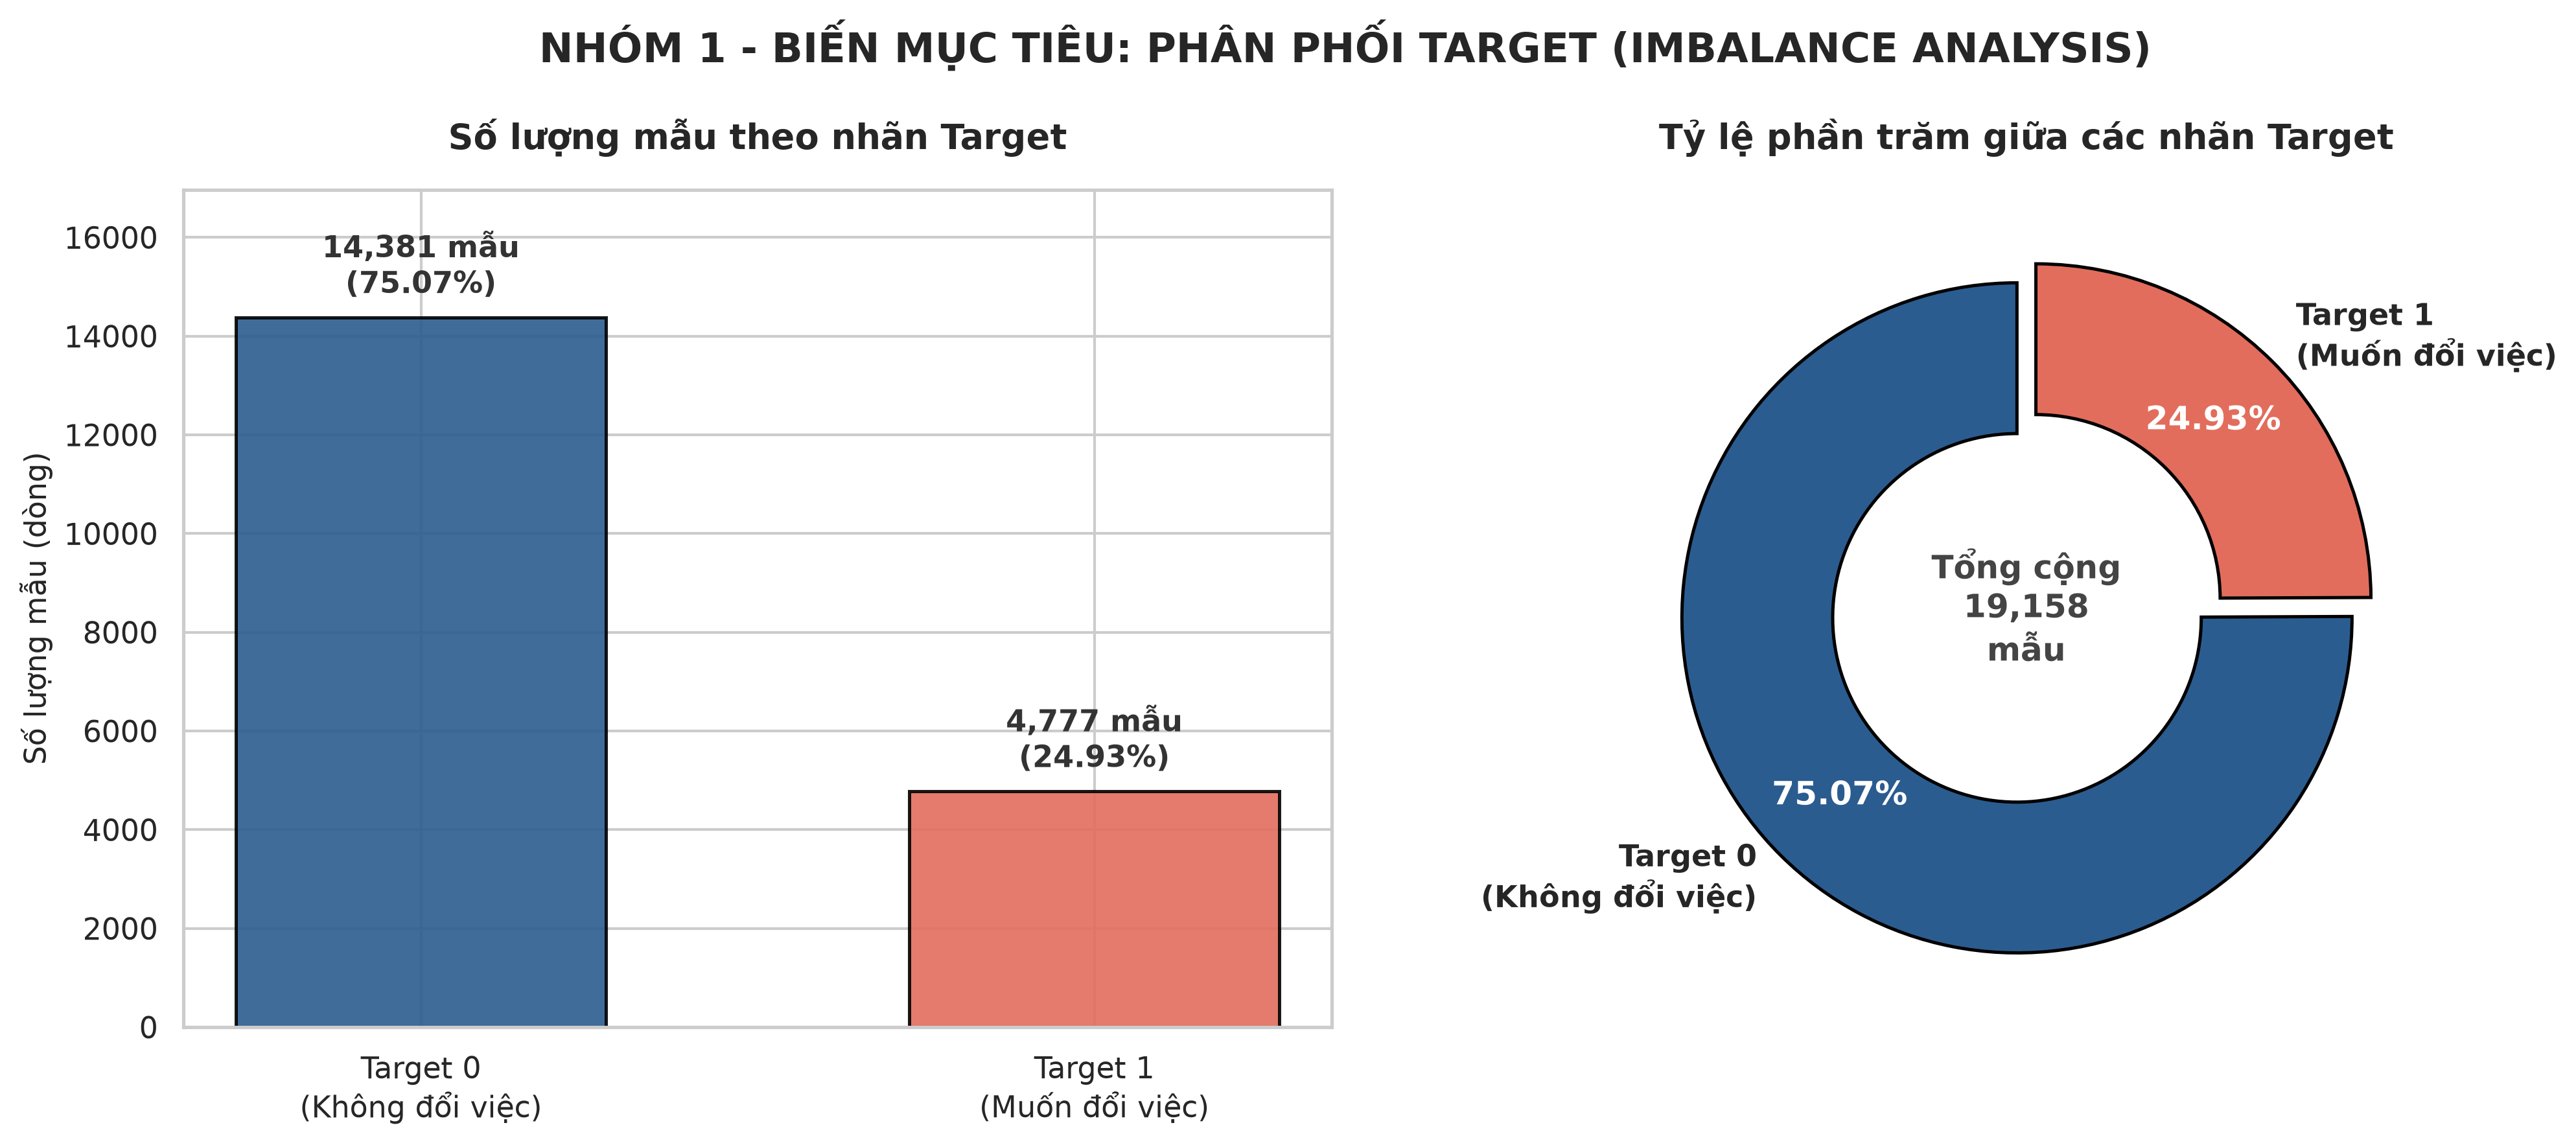
\includegraphics[width=0.96\textwidth]{group1_target_distribution.png}
  \caption{Phân phối nhãn và tỷ lệ lớp dương của bộ dữ liệu.}
  \label{fig:target-distribution}
\end{figure}

\section{Phân tích biến số}

\begin{table}[H]
\centering
\caption{Thống kê hai biến số gốc}\label{tab:numeric-summary}
\begin{tabular}{lrrrrrr}
\toprule
\textbf{Biến} & \textbf{Min} & \textbf{Q1} & \textbf{Median} & \textbf{Mean} & \textbf{Q3} & \textbf{Max} \\
\midrule
Chỉ số phát triển thành phố & 0,448 & 0,740 & 0,903 & 0,829 & 0,920 & 0,949 \\
Giờ đào tạo & 1 & 23 & 47 & 65,37 & 88 & 336 \\
\bottomrule
\end{tabular}
\end{table}

\code{training\_hours} có mean lớn hơn median và đuôi phải kéo dài đến 336 giờ, do đó nhóm tạo thêm $\log(1+x)$. \code{city\_development\_index} tập trung nhiều ở vùng cao nhưng có nhóm thành phố phát triển thấp; các hình theo nhãn cho thấy biến này có khả năng phân tách đáng kể.

\begin{figure}[H]
  \centering
  \begin{subfigure}[t]{0.49\textwidth}
    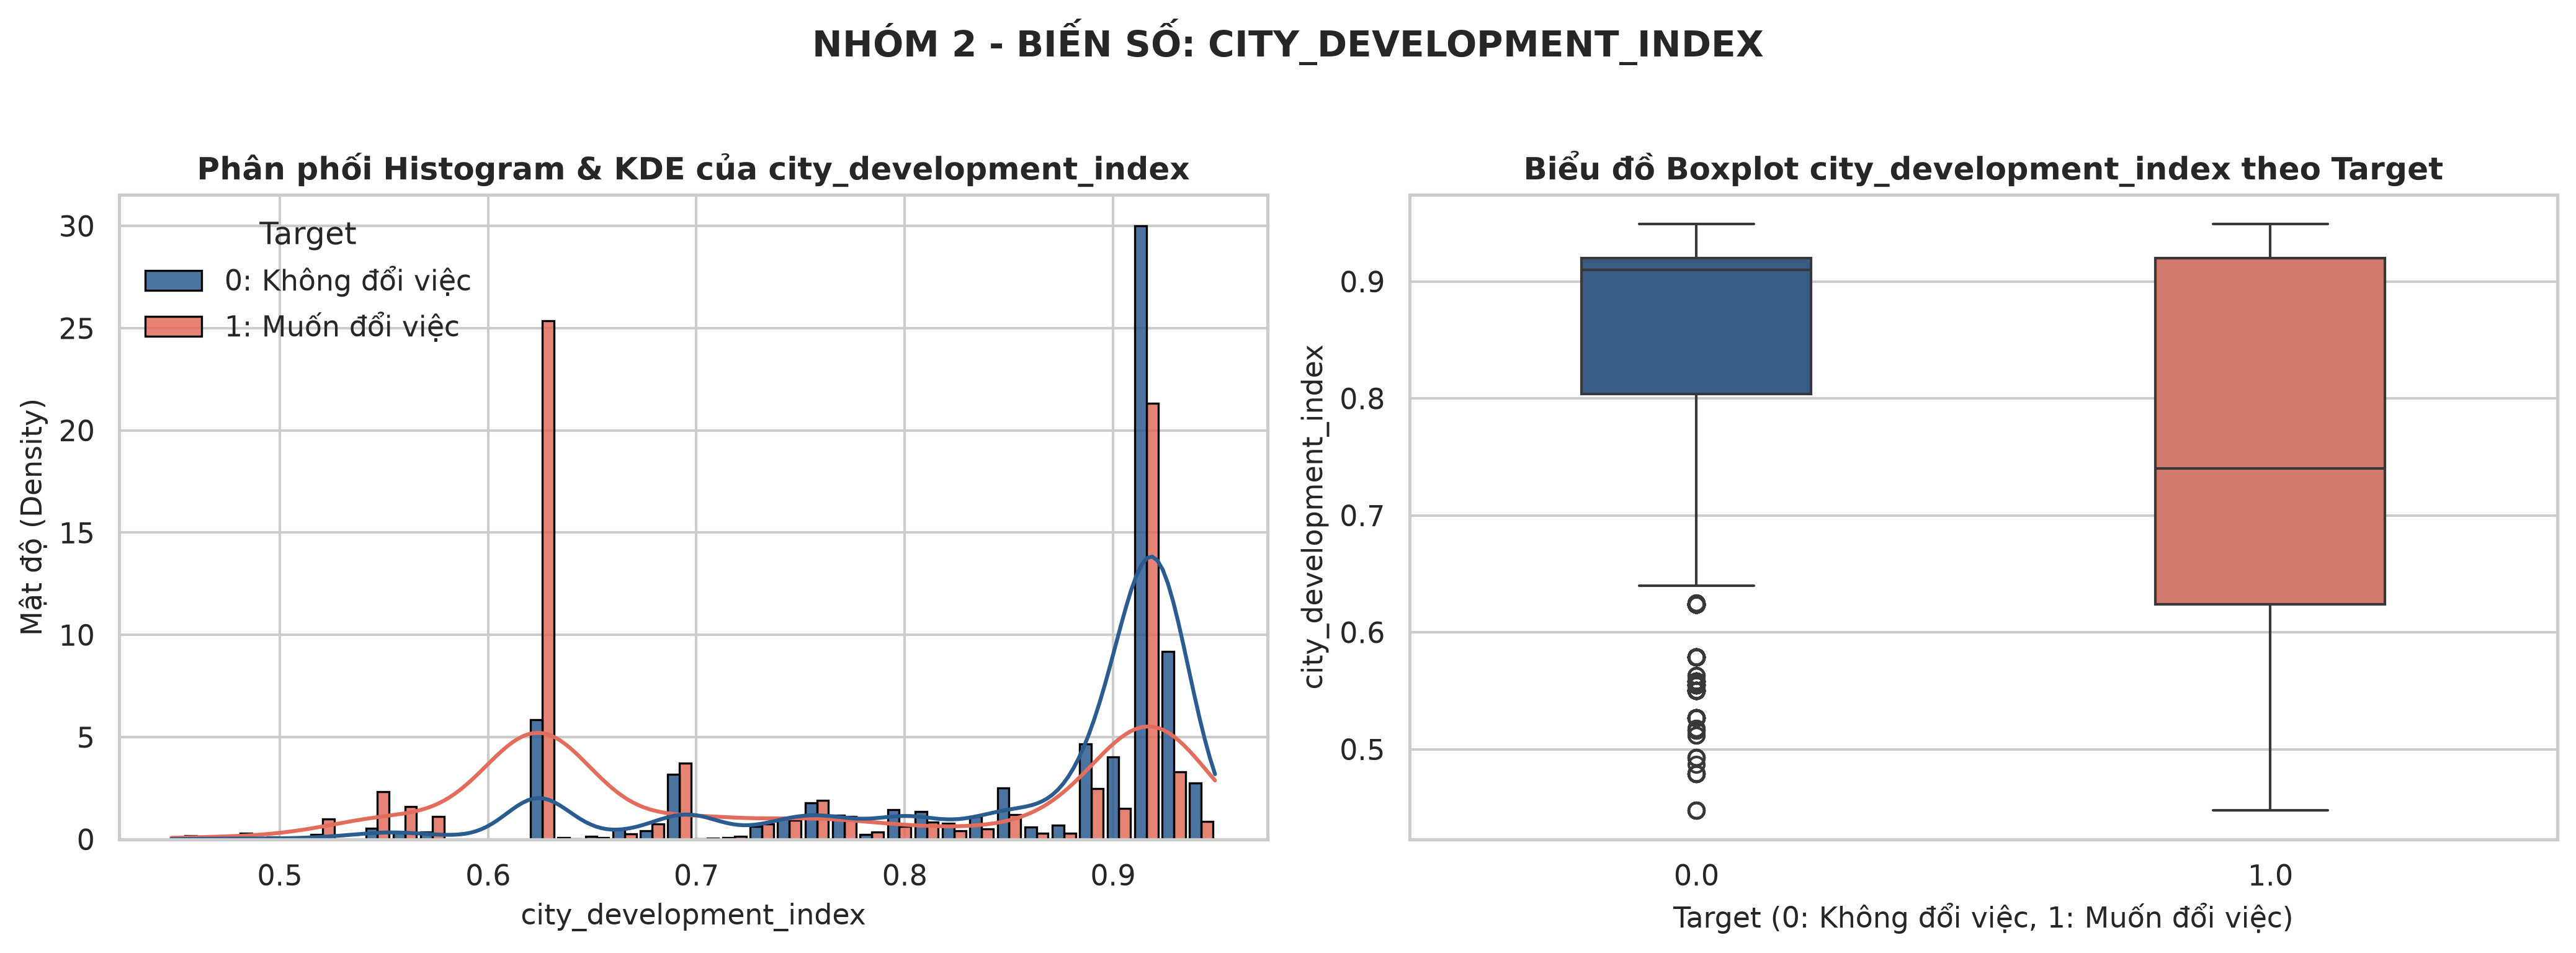
\includegraphics[width=\textwidth]{group2_num_city_development_index.png}
    \caption{Chỉ số phát triển thành phố.}
  \end{subfigure}
  \hfill
  \begin{subfigure}[t]{0.49\textwidth}
    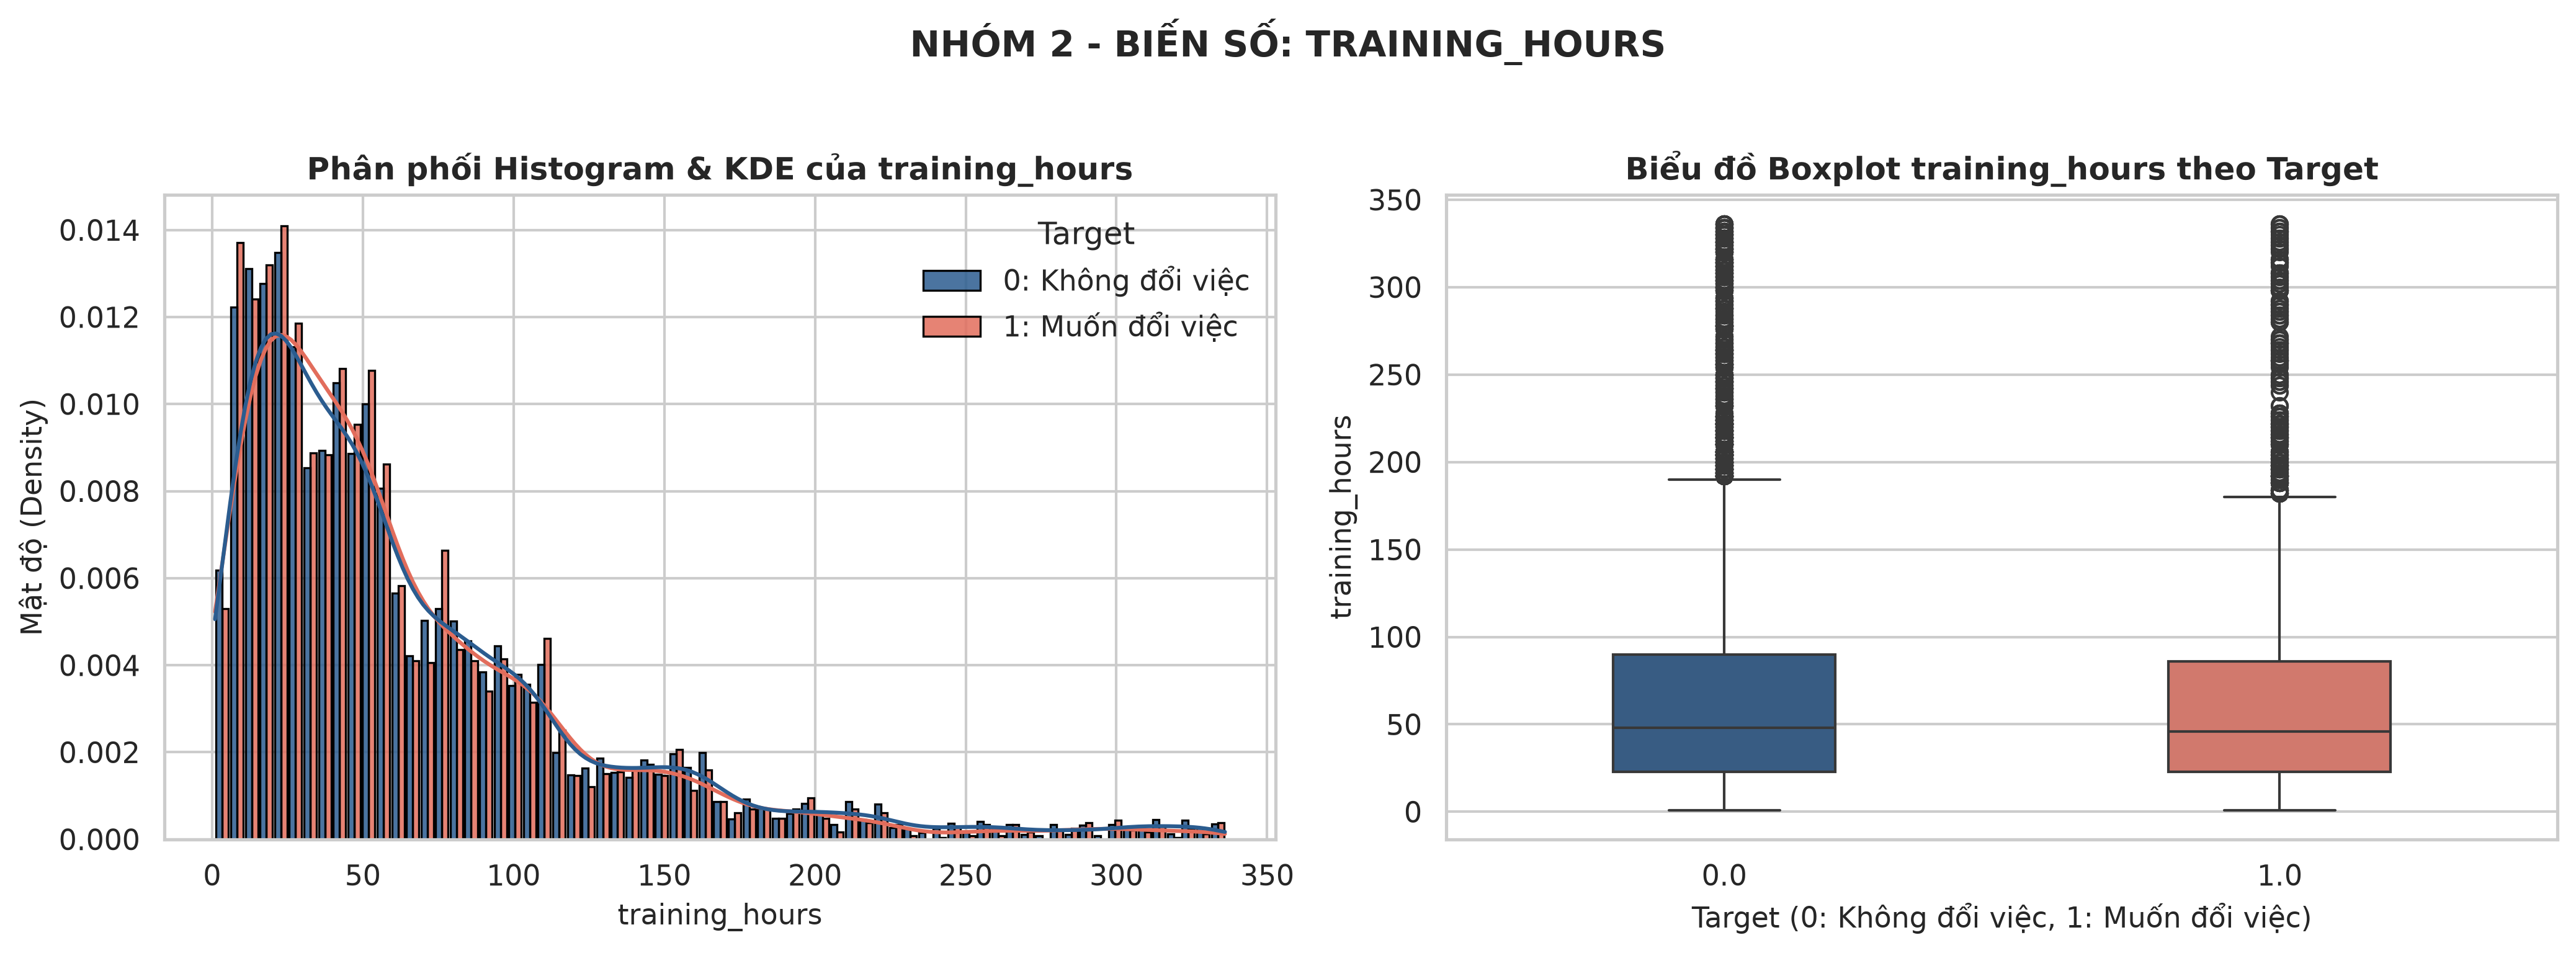
\includegraphics[width=\textwidth]{group2_num_training_hours.png}
    \caption{Số giờ đào tạo.}
  \end{subfigure}
  \caption{Phân phối biến số và quan hệ với target.}
  \label{fig:numerical-eda}
\end{figure}

\section{Phân tích biến phân loại và thứ bậc}

Một số khác biệt đáng chú ý từ EDA:

\begin{itemize}
  \item ứng viên không có kinh nghiệm liên quan có tỷ lệ lớp dương 33,84\%, cao hơn nhóm có kinh nghiệm liên quan (21,47\%);
  \item người học khóa toàn thời gian có tỷ lệ lớp dương 38,09\%, trong khi nhóm không tham gia đại học là 21,14\%;
  \item nhóm trình độ Graduate chiếm 60,54\% dữ liệu và có tỷ lệ lớp dương 27,98\%; PhD là 14,01\%;
  \item hồ sơ thiếu giới tính có tỷ lệ lớp dương 30,81\%, cao hơn nhóm Male (22,78\%);
  \item \code{city} có 123 mức. Mỗi city liên kết với một giá trị chỉ số phát triển cố định; để giảm dư thừa và số chiều, pipeline truyền thống loại \code{city}, trong khi ResNet và TabM vẫn giữ dưới dạng embedding.
\end{itemize}

\begin{figure}[H]
  \centering
  \begin{subfigure}[t]{0.49\textwidth}
    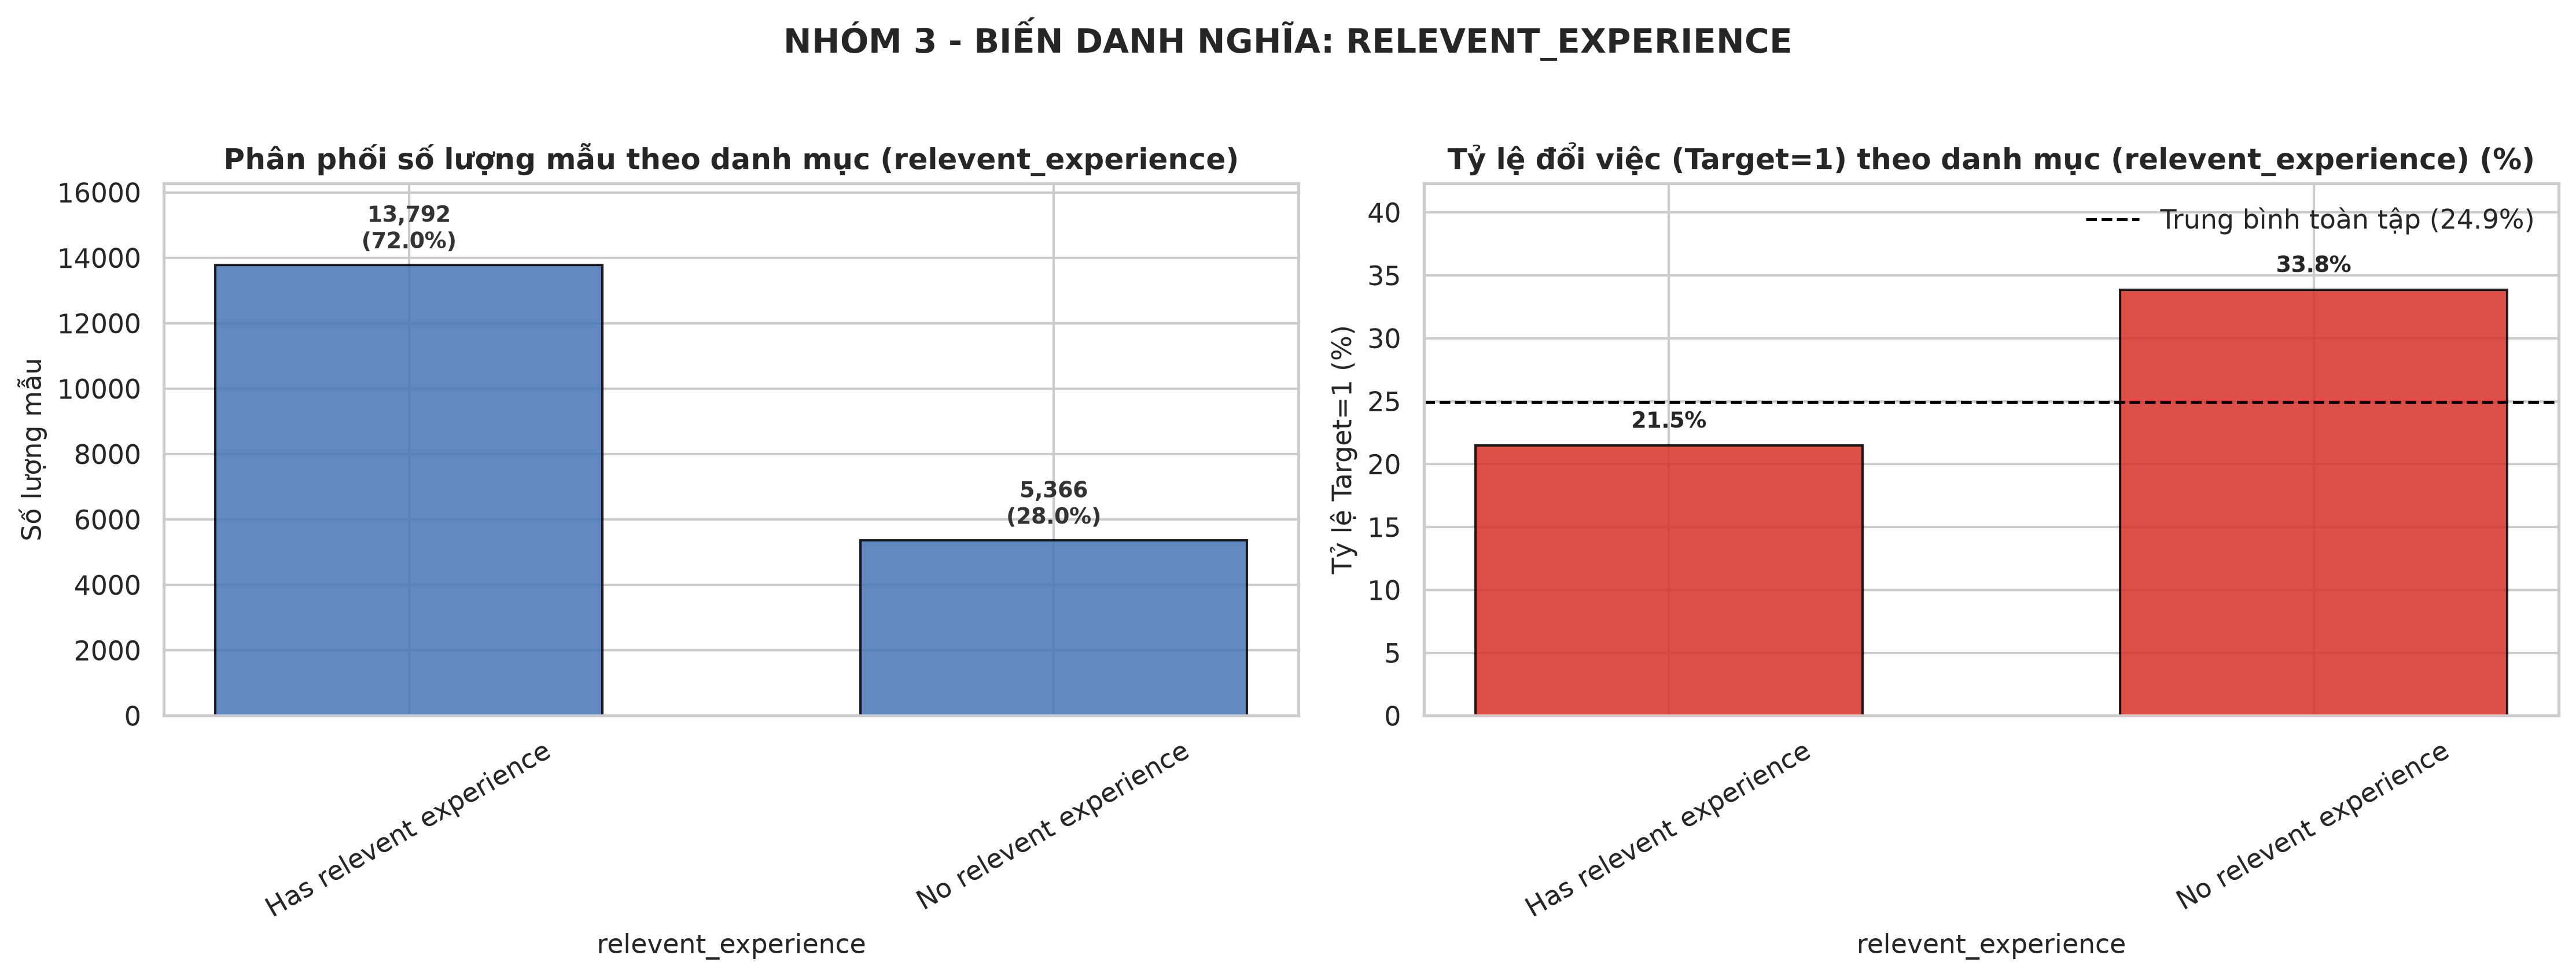
\includegraphics[width=\textwidth]{group3_nominal_relevent_experience.png}
    \caption{Kinh nghiệm liên quan.}
  \end{subfigure}
  \hfill
  \begin{subfigure}[t]{0.49\textwidth}
    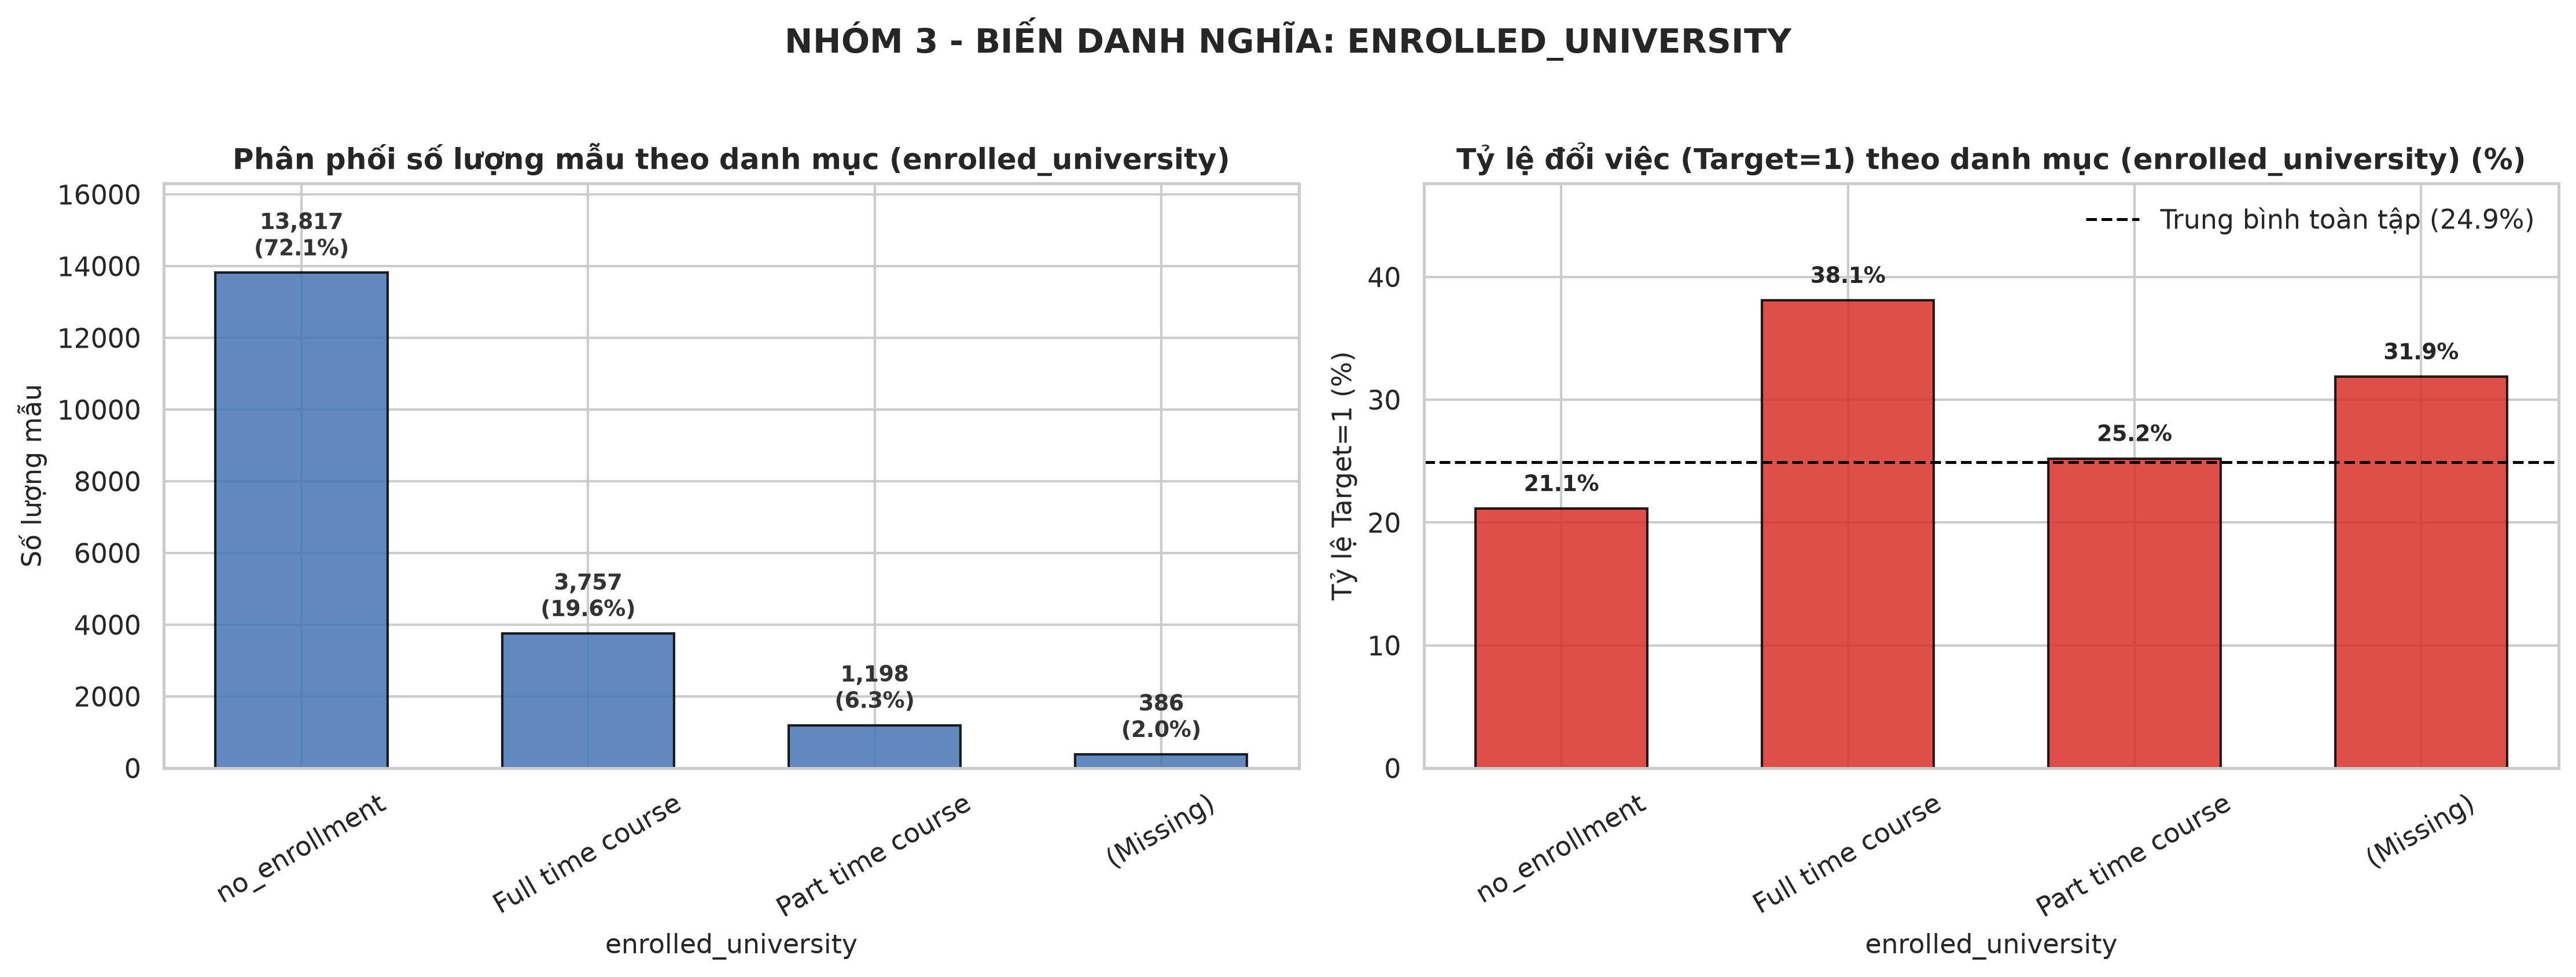
\includegraphics[width=\textwidth]{group3_nominal_enrolled_university.png}
    \caption{Tình trạng học đại học.}
  \end{subfigure}
  \caption{Ví dụ phân tích các thuộc tính danh nghĩa.}
  \label{fig:nominal-eda}
\end{figure}

\begin{figure}[H]
  \centering
  \begin{subfigure}[t]{0.49\textwidth}
    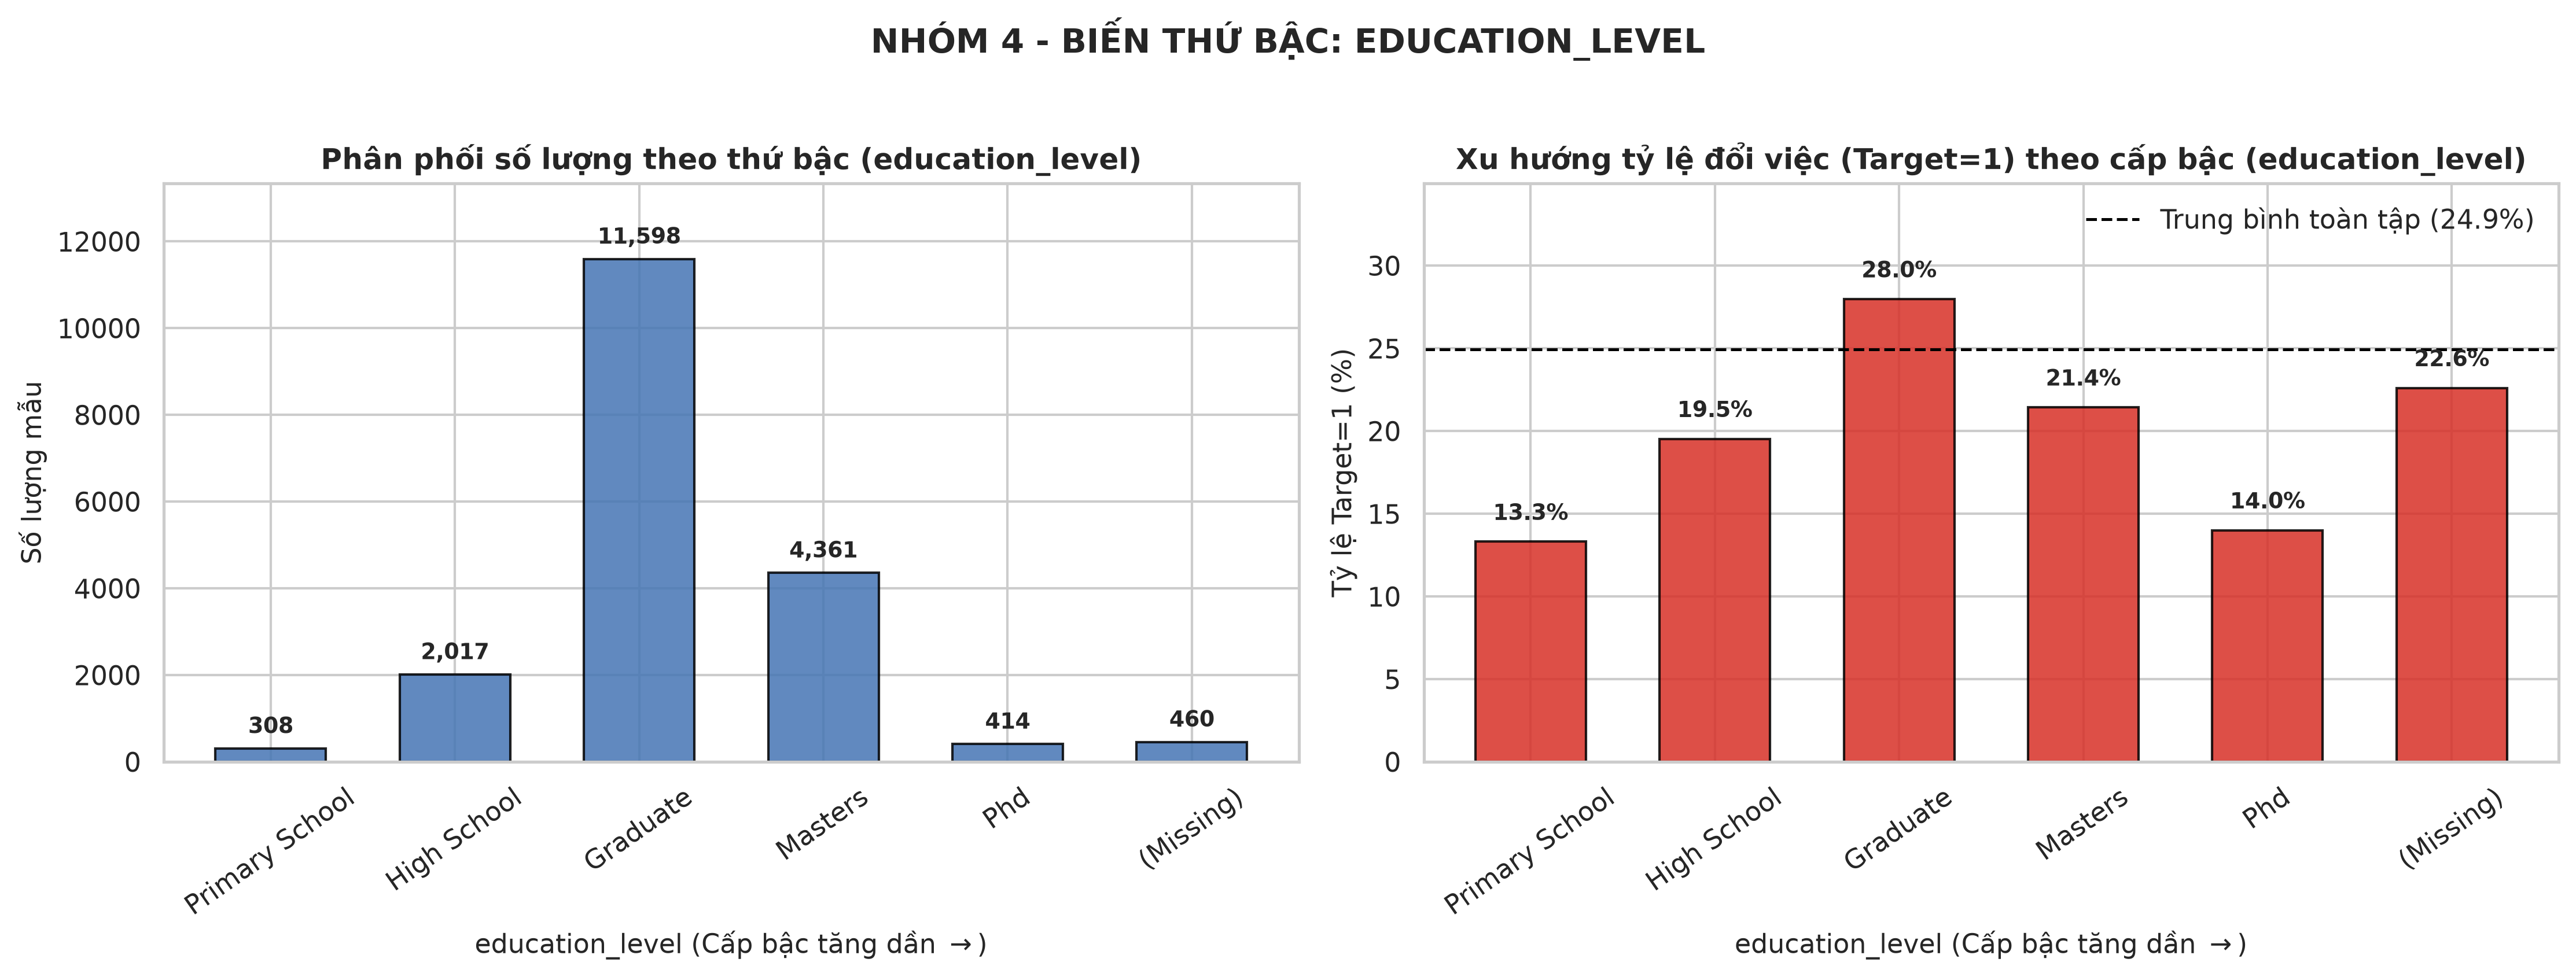
\includegraphics[width=\textwidth]{group4_ordinal_education_level.png}
    \caption{Trình độ học vấn.}
  \end{subfigure}
  \hfill
  \begin{subfigure}[t]{0.49\textwidth}
    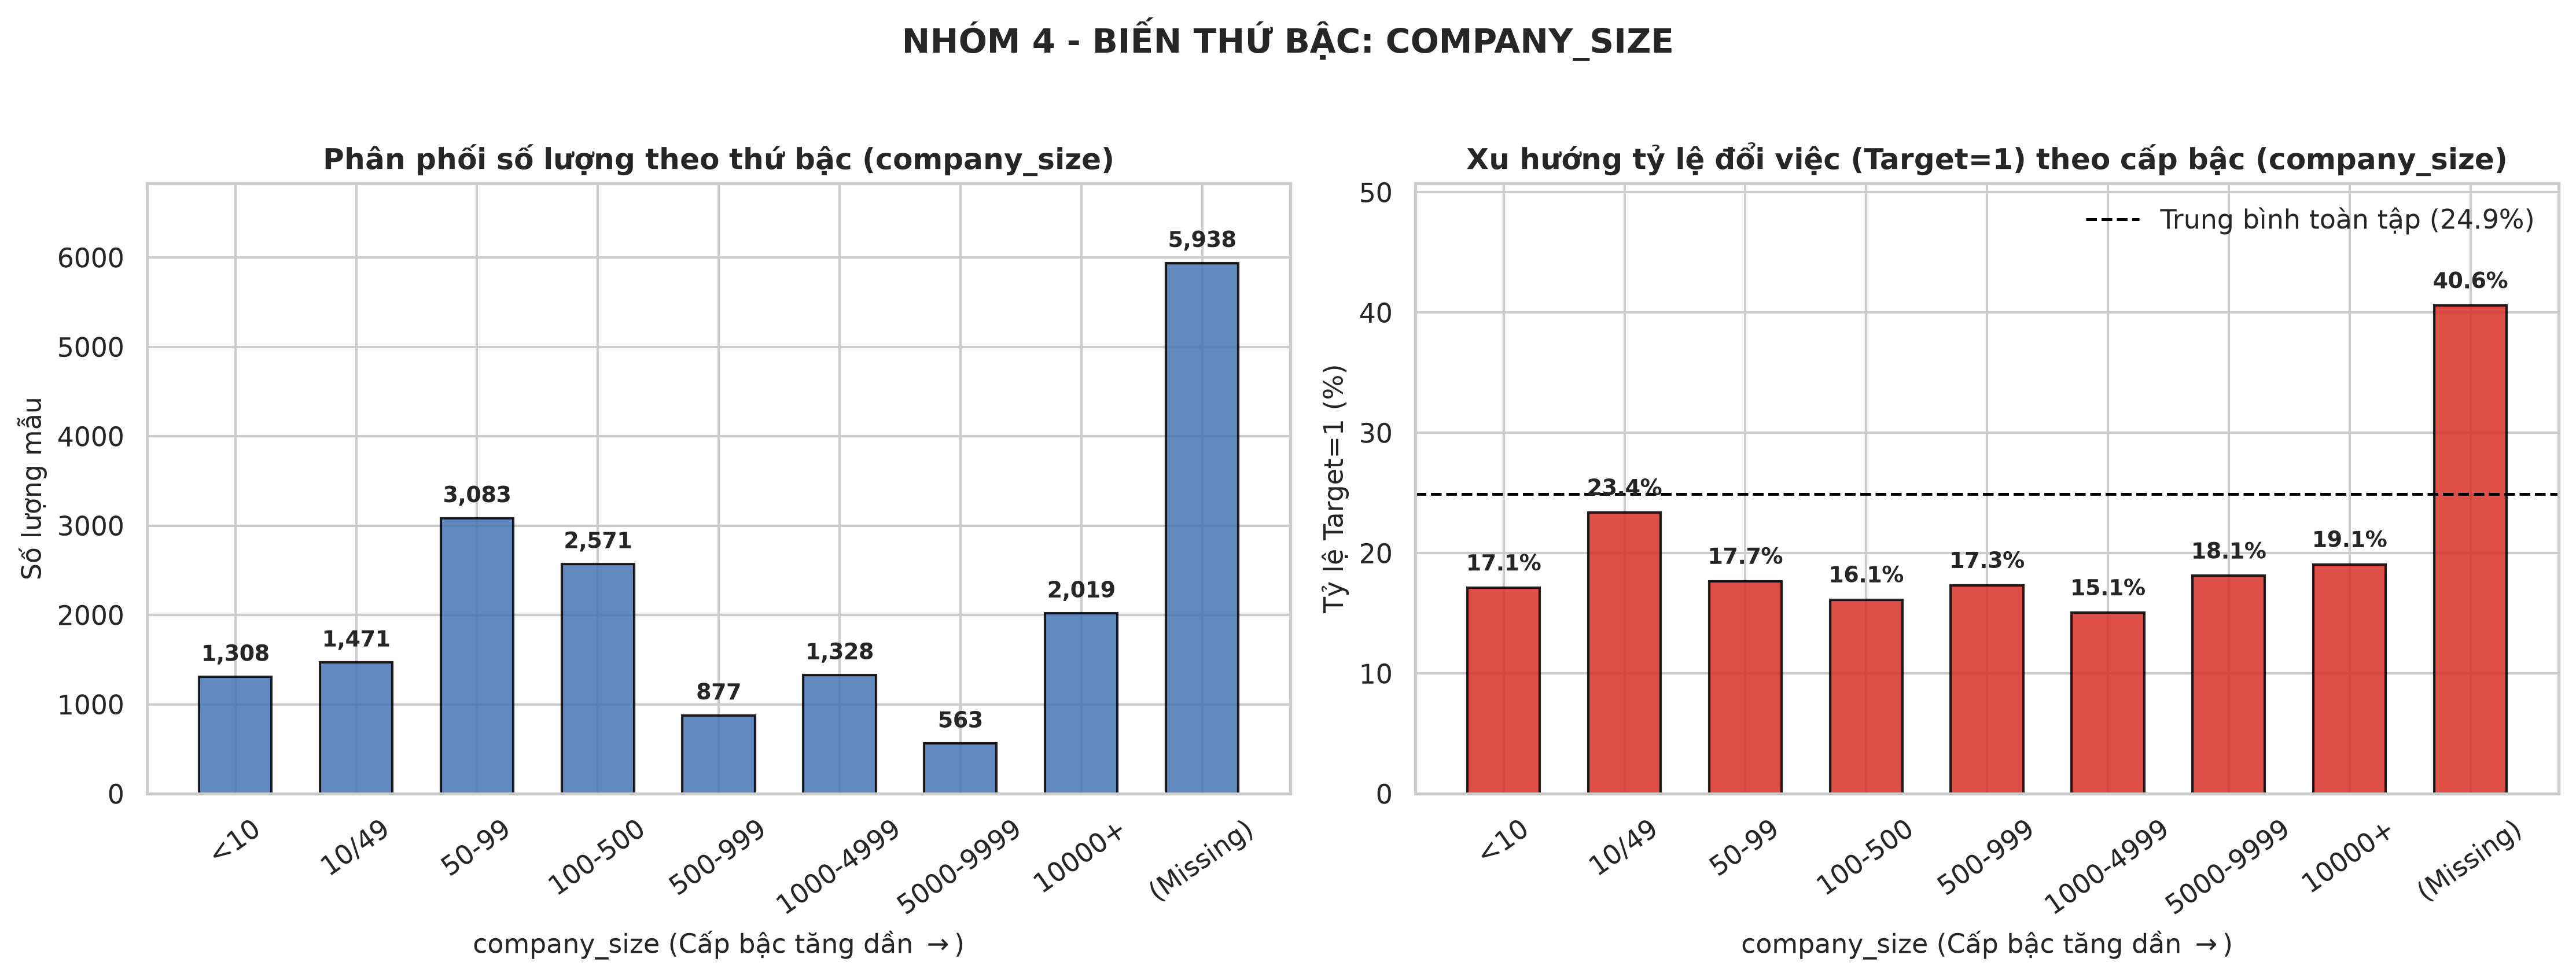
\includegraphics[width=\textwidth]{group4_ordinal_company_size.png}
    \caption{Quy mô công ty.}
  \end{subfigure}
  \caption{Ví dụ phân tích các thuộc tính thứ bậc.}
  \label{fig:ordinal-eda}
\end{figure}

\section{Dữ liệu khuyết và tín hiệu missingness}

Có tám cột chứa giá trị khuyết. Đáng chú ý nhất là \code{company\_type} (32,05\%) và \code{company\_size} (30,99\%). Missingness không hoàn toàn ngẫu nhiên: tỷ lệ lớp dương khi \code{company\_size} bị thiếu là 40,59\%, cao hơn 22,68 điểm phần trăm so với nhóm quan sát được. Chênh lệch tương ứng của \code{company\_type} là 20,45 điểm phần trăm. Vì vậy, thay vì chỉ điền mode, pipeline giữ riêng trạng thái \code{Unknown}/$-1$ và thêm missing indicator cho hai cột này.

\begin{figure}[H]
  \centering
  \begin{subfigure}[t]{0.49\textwidth}
    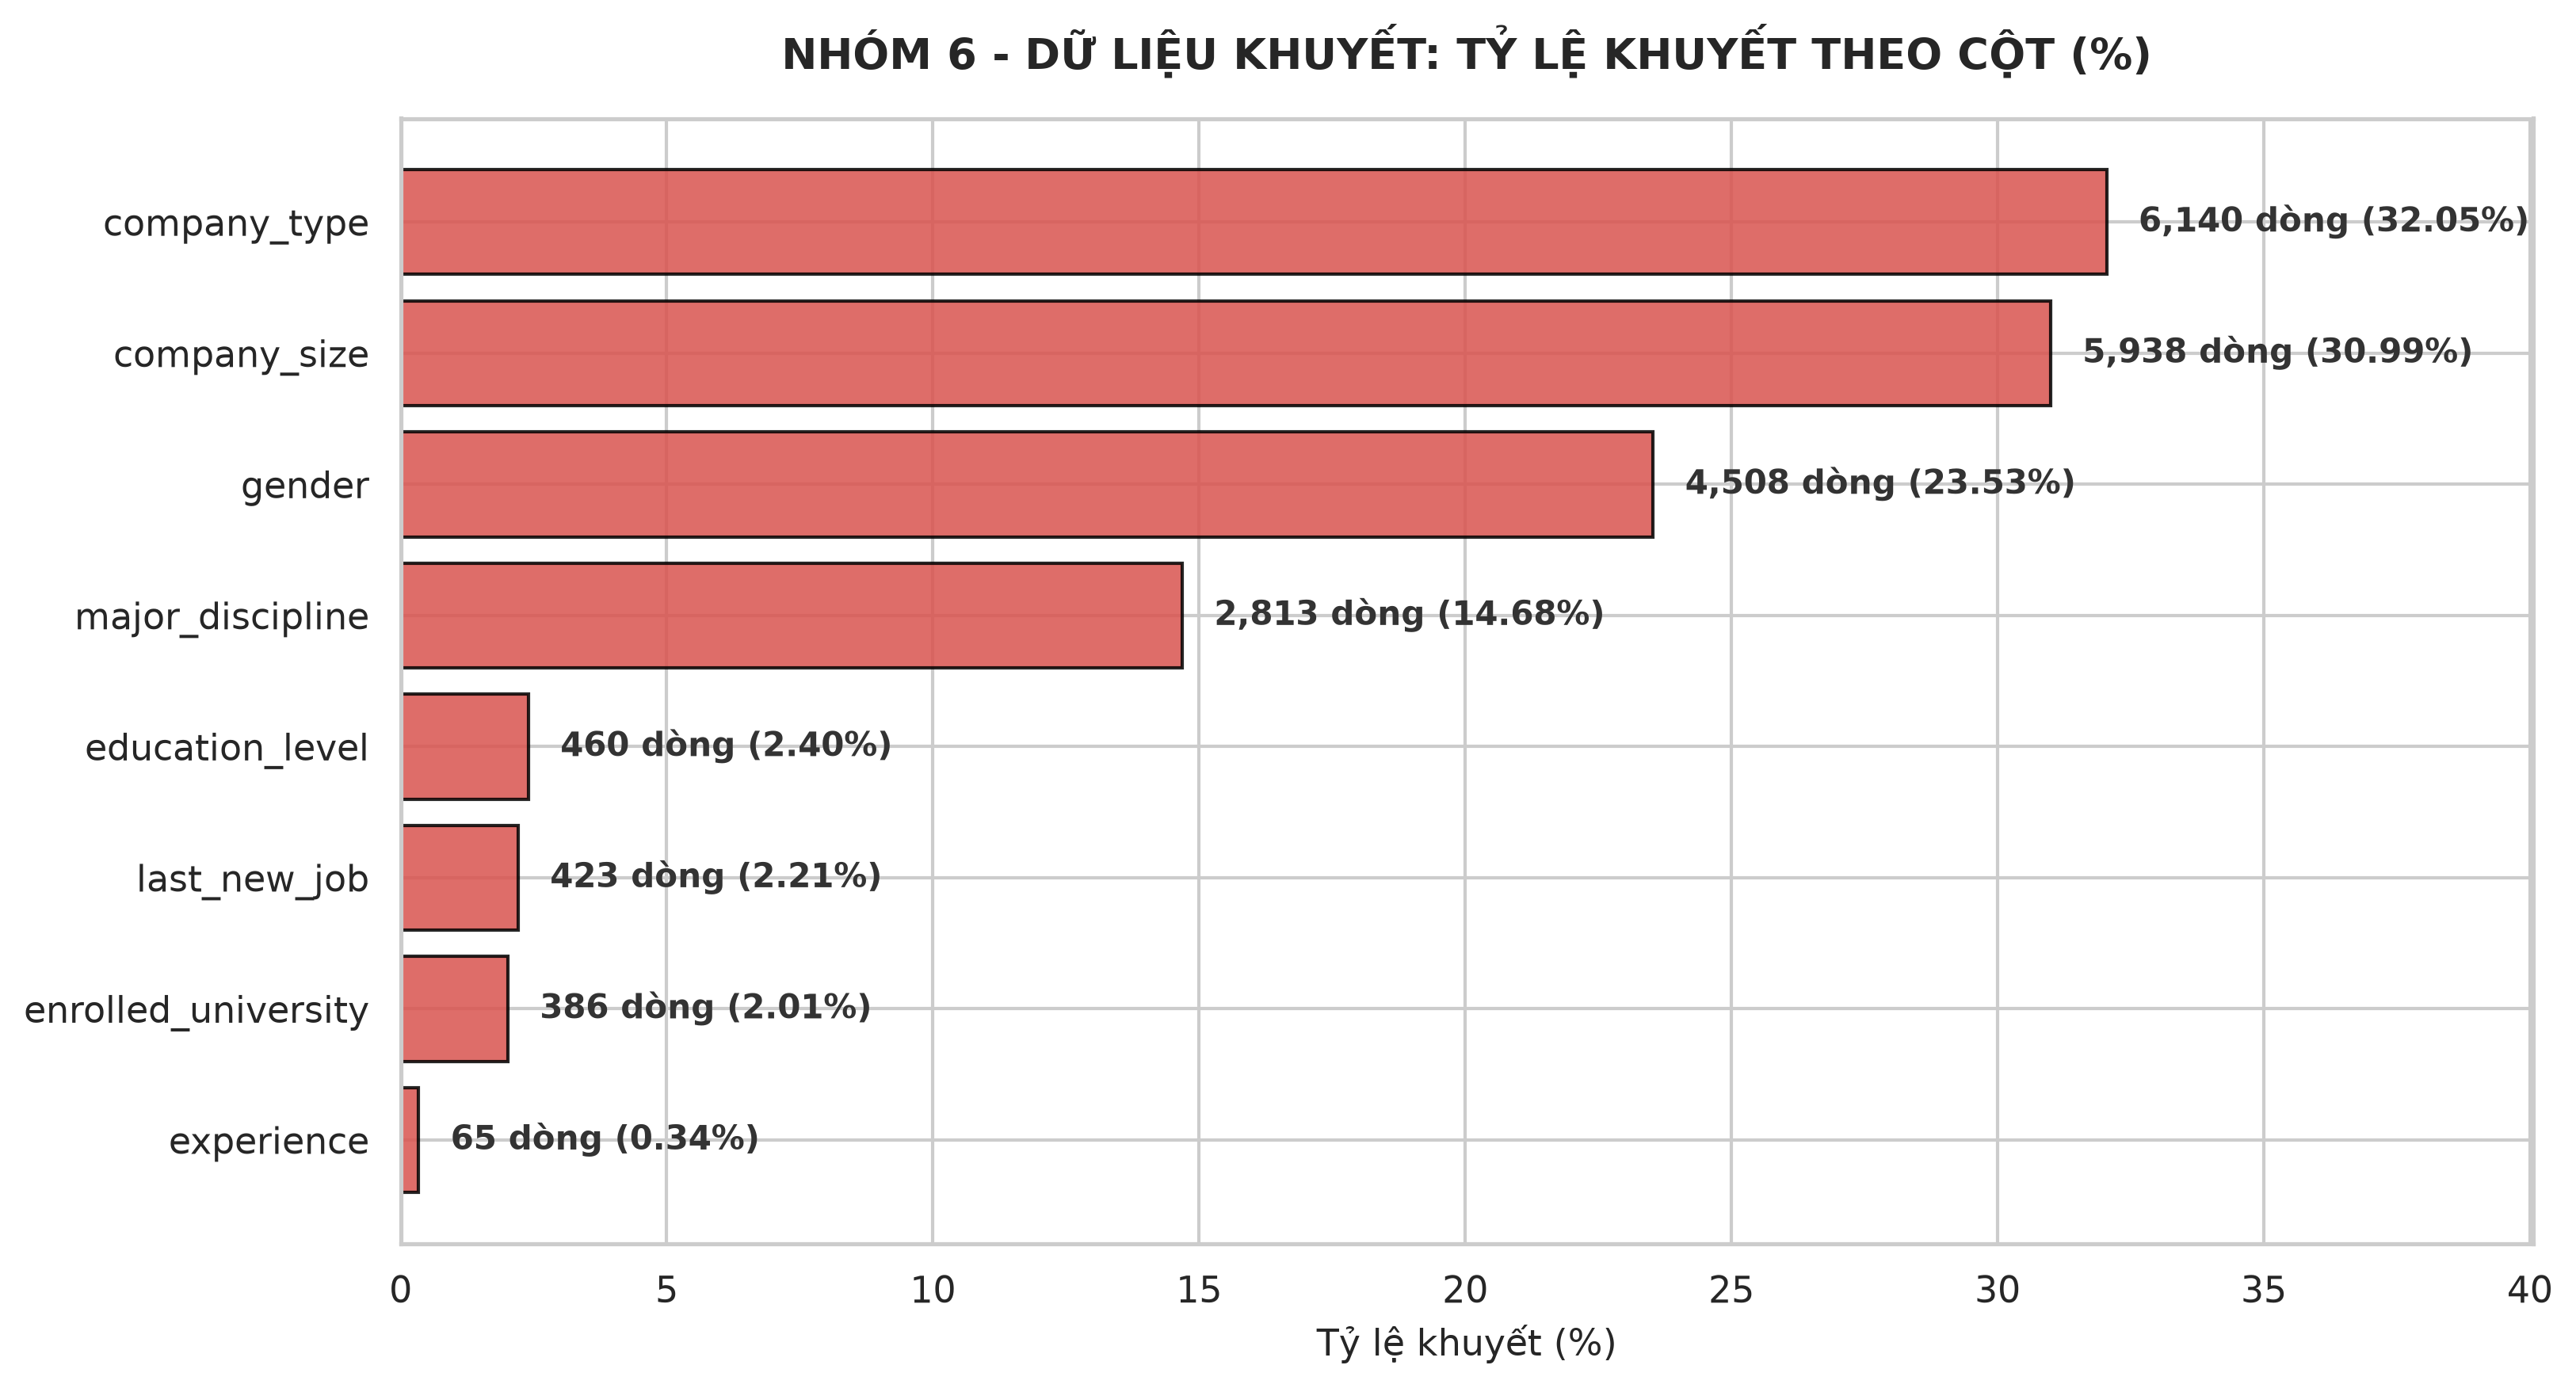
\includegraphics[width=\textwidth]{group6_missing_values_bar.png}
    \caption{Tỷ lệ giá trị khuyết.}
  \end{subfigure}
  \hfill
  \begin{subfigure}[t]{0.49\textwidth}
    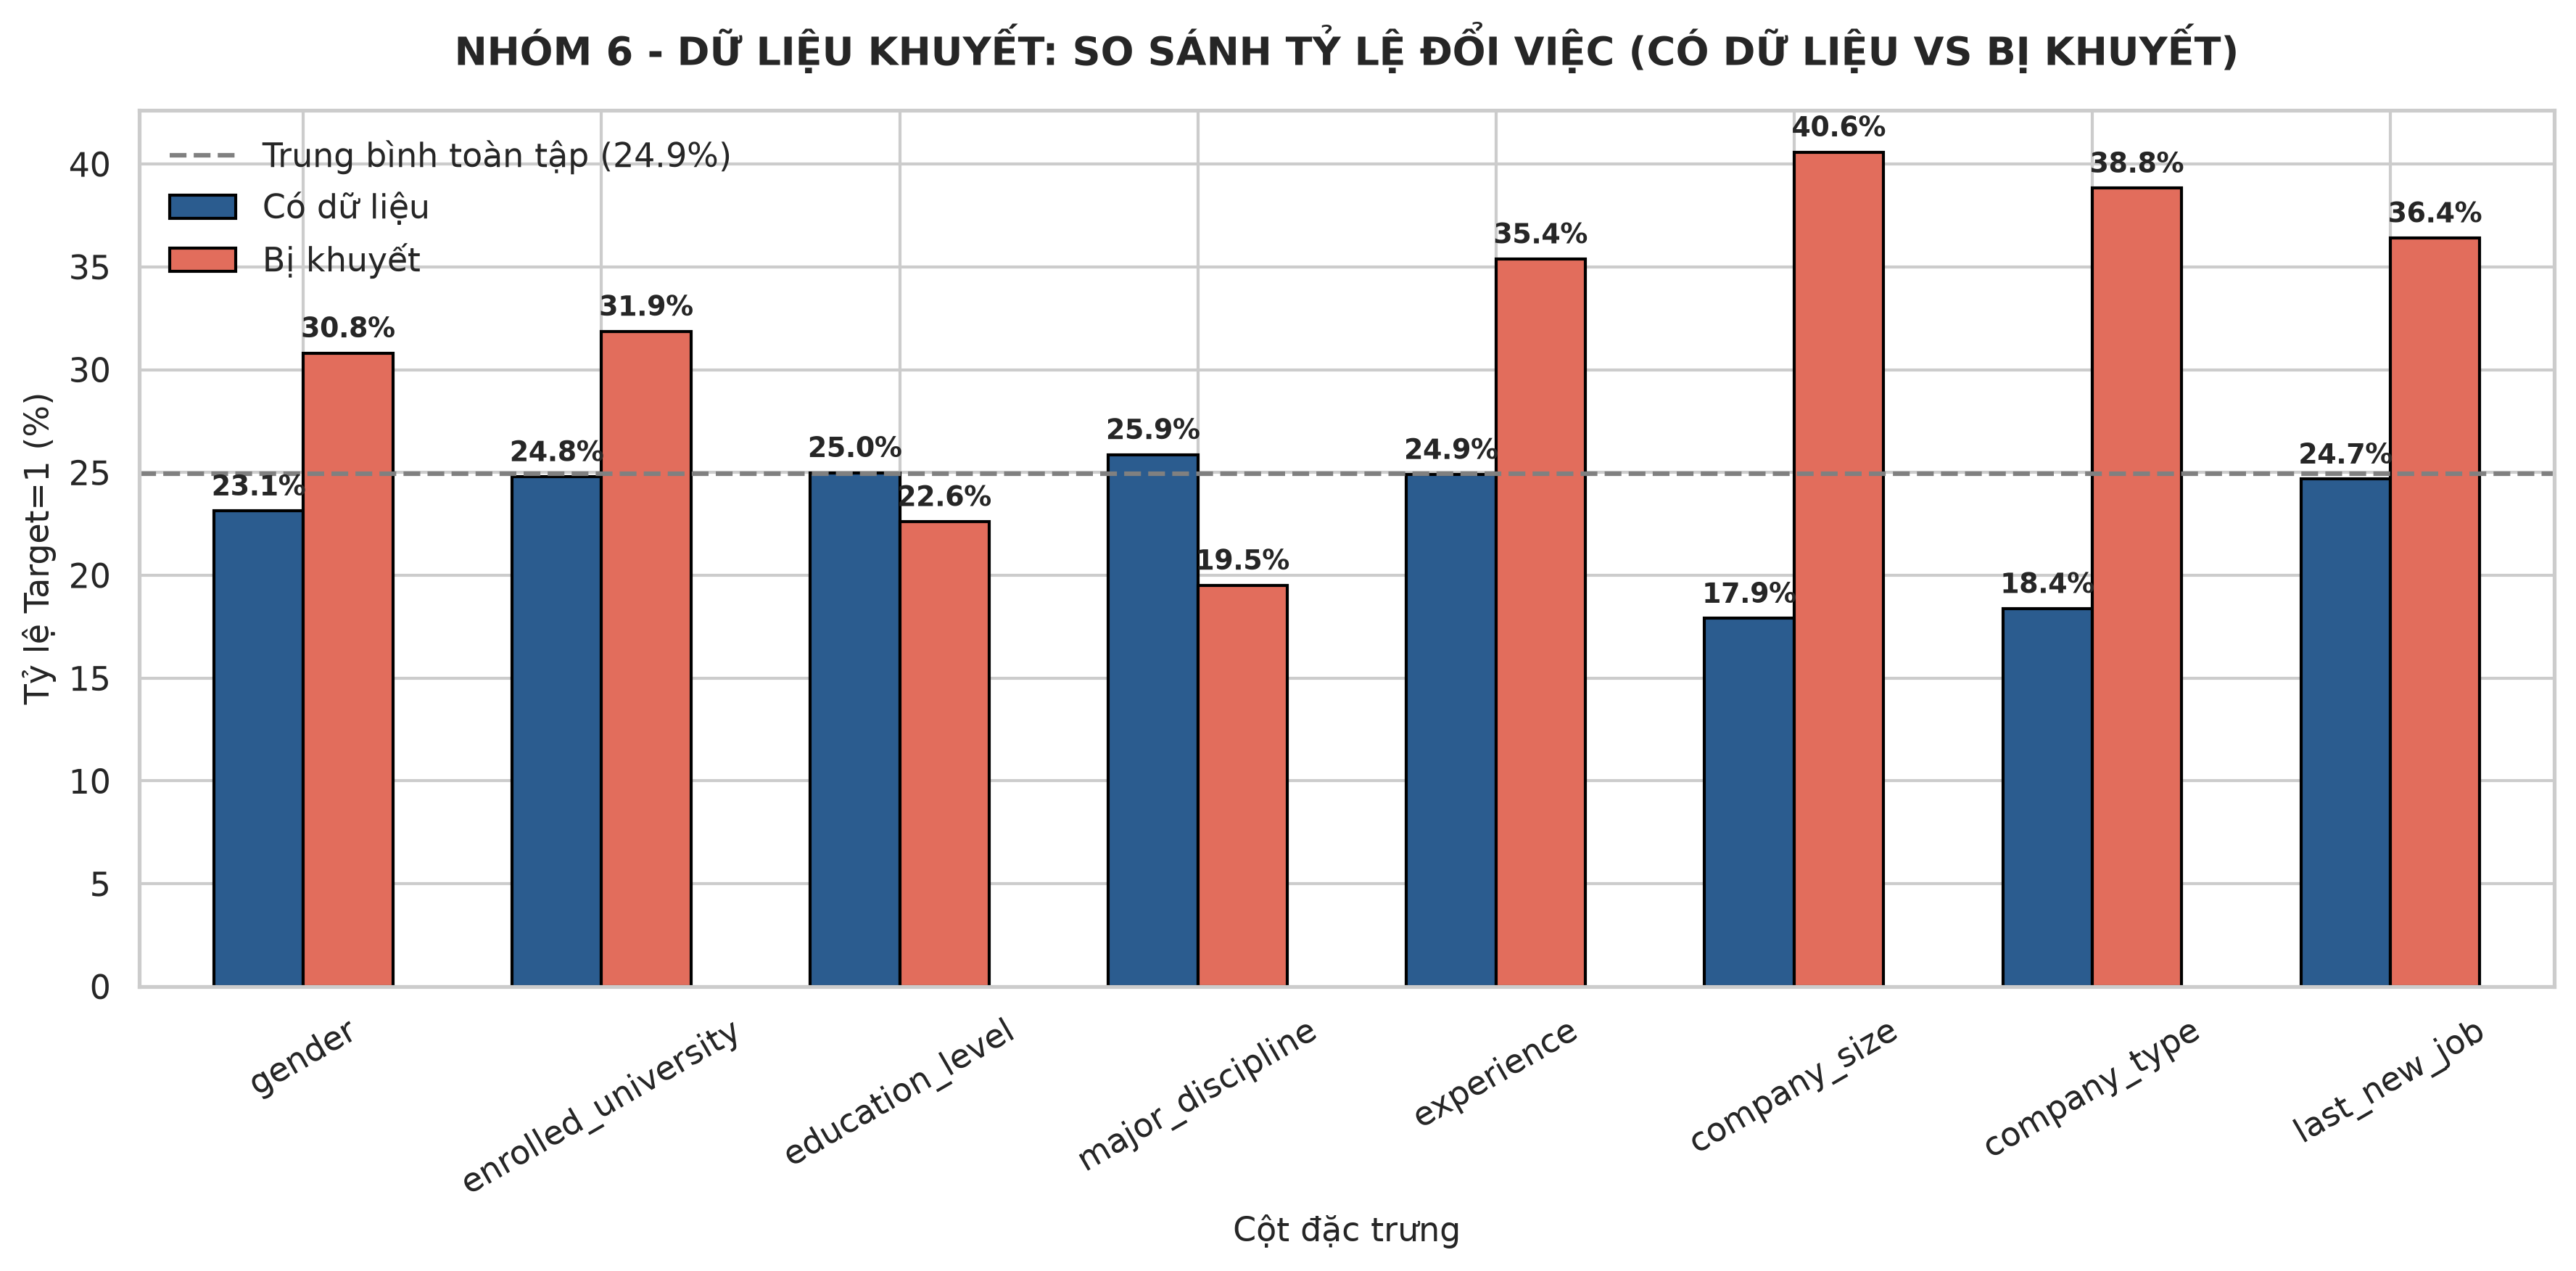
\includegraphics[width=\textwidth]{group6_missingness_vs_target.png}
    \caption{Target rate theo trạng thái khuyết.}
  \end{subfigure}
  \caption{Phân tích missingness và mối liên hệ với target.}
  \label{fig:missingness}
\end{figure}

\section{Tương quan và kết luận EDA}

Ma trận Spearman cho thấy \code{city\_development\_index} và các biến dẫn xuất của nó có quan hệ đáng kể với target. Tuy nhiên, tương quan cặp không đủ mô tả các tương tác phi tuyến giữa kinh nghiệm, trình độ, thành phố và trạng thái hồ sơ. Kết luận EDA dẫn đến bốn quyết định: (i) giữ missingness như một tín hiệu; (ii) tạo đặc trưng tương tác; (iii) sử dụng cả mô hình tuyến tính và cây phi tuyến; (iv) chọn chỉ số đánh giá phù hợp với lệch lớp.

\begin{figure}[H]
  \centering
  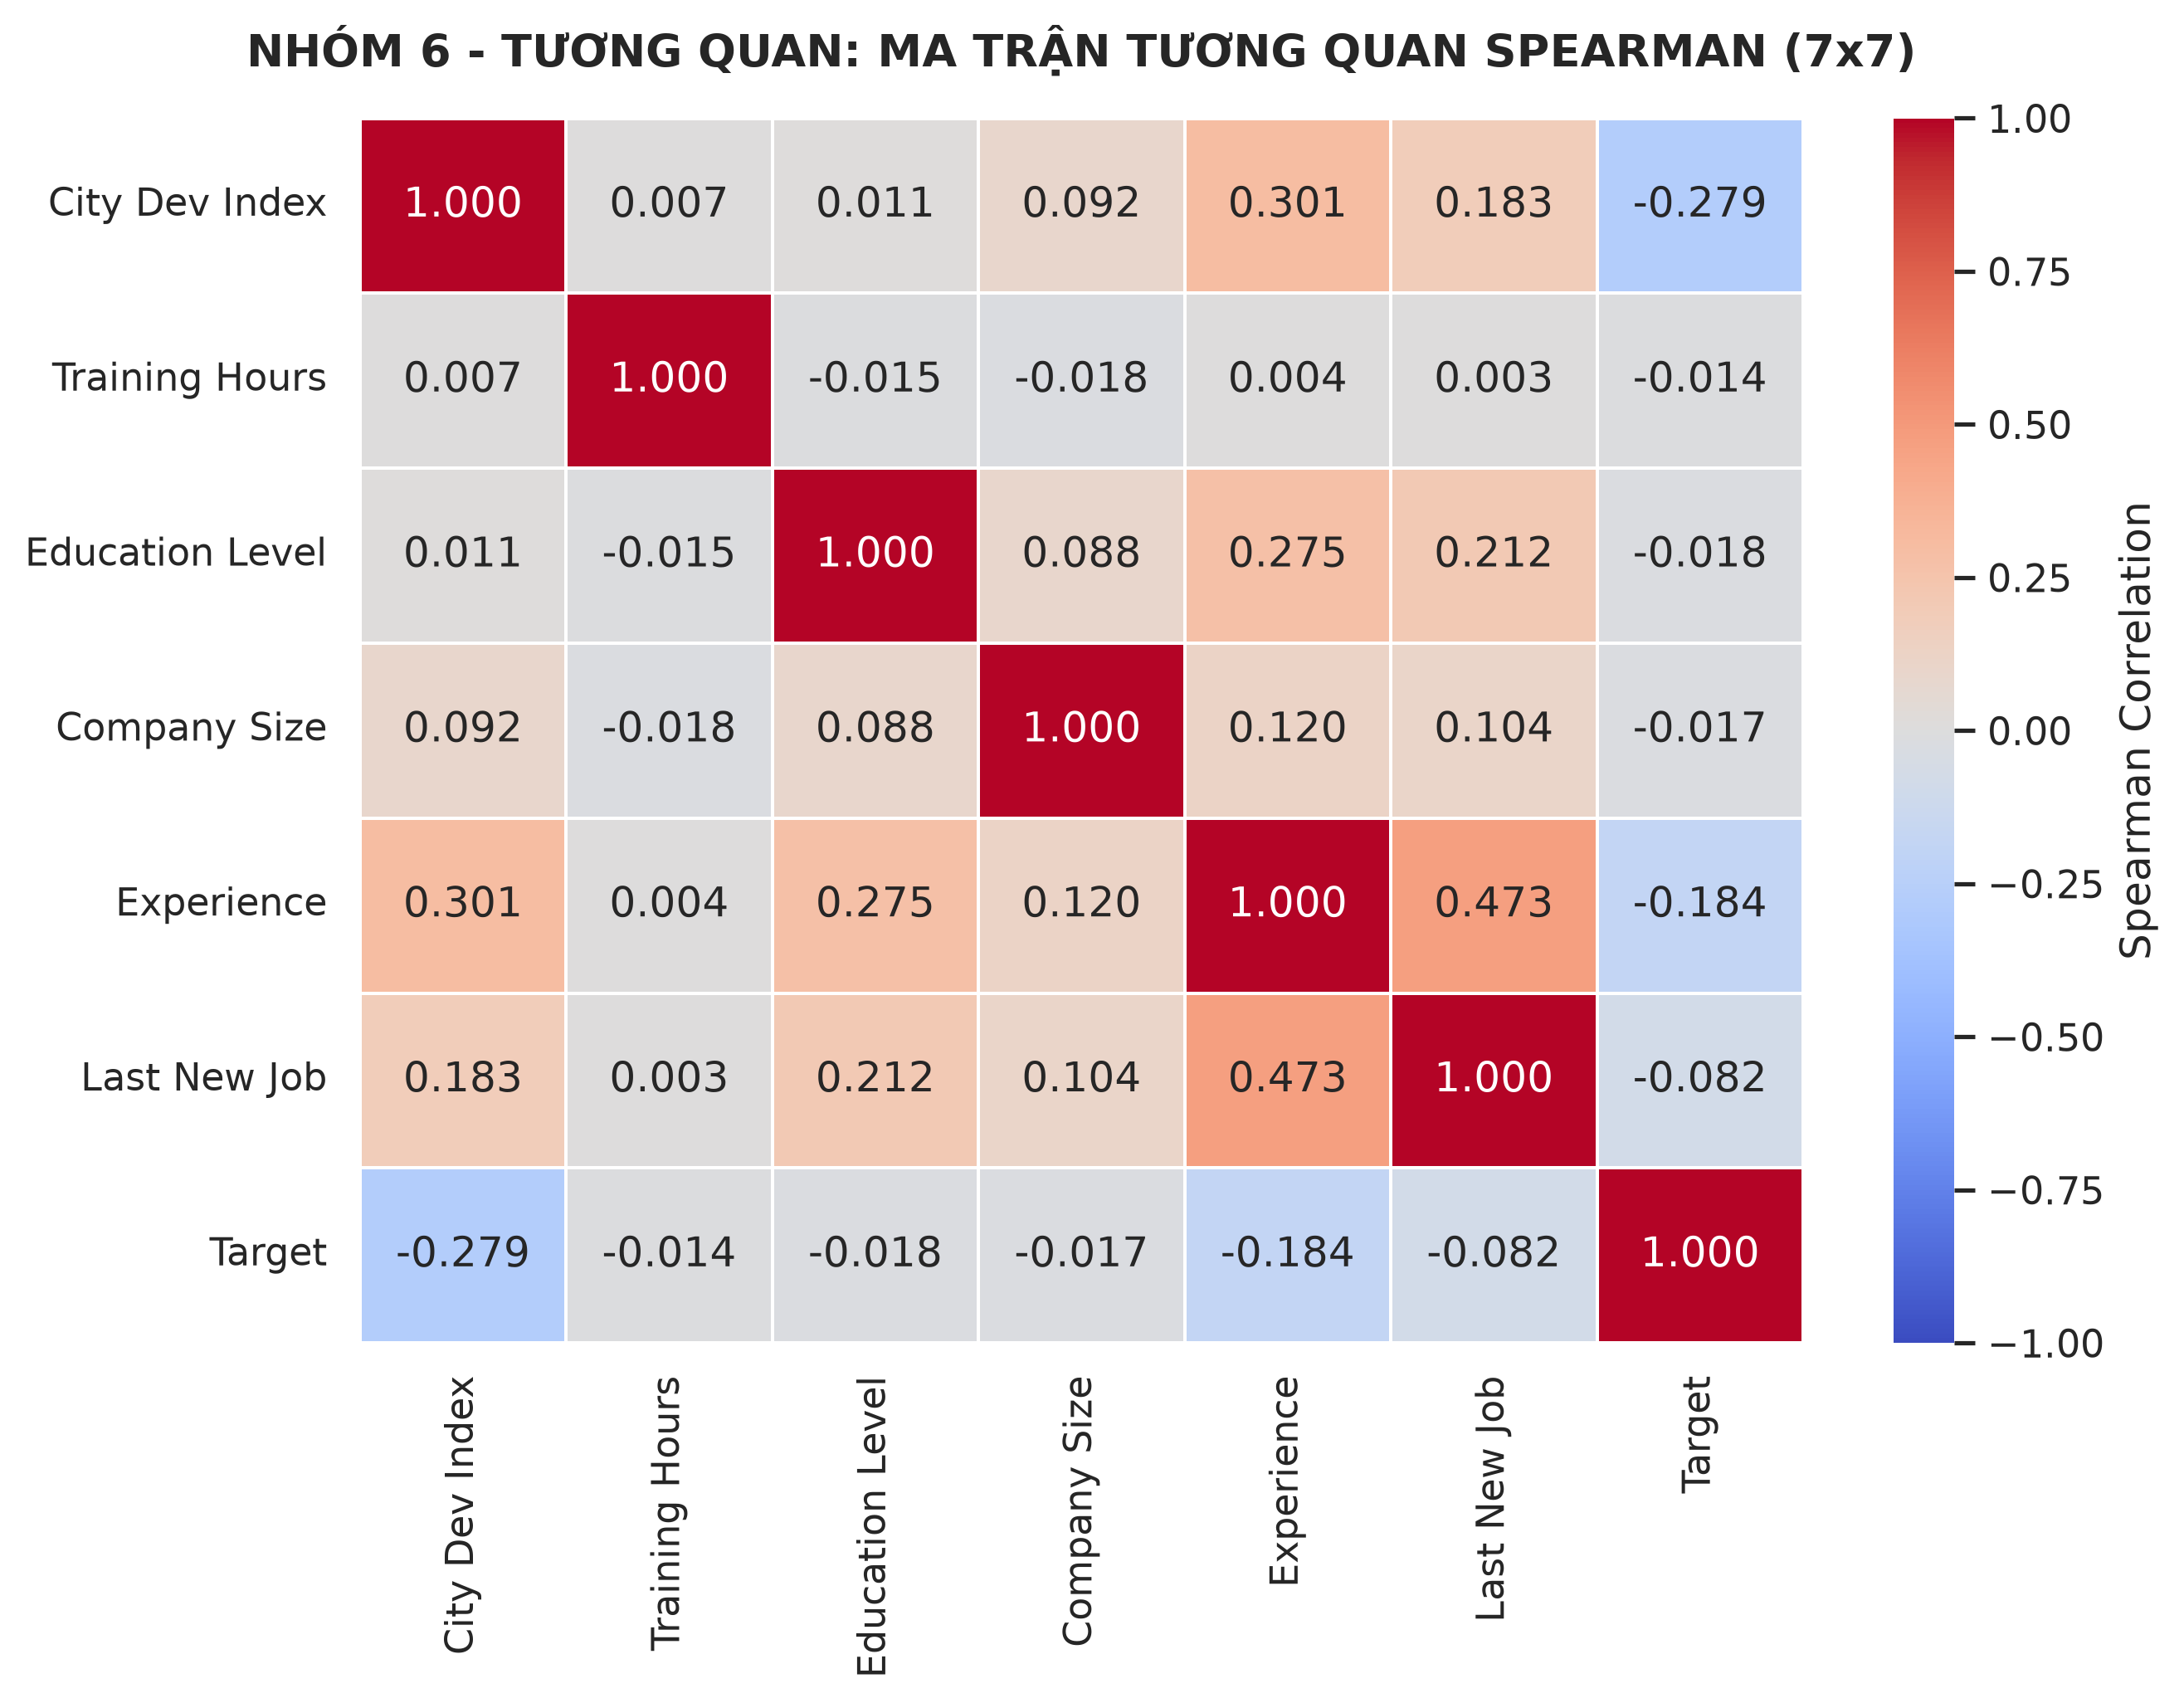
\includegraphics[width=0.78\textwidth]{group6_correlation_matrix.png}
  \caption{Ma trận tương quan Spearman của các biến số/thứ bậc.}
  \label{fig:correlation}
\end{figure}

% =============================================================================
\chapter{Thiết kế pipeline và phương pháp đánh giá}
% =============================================================================

\section{Protocol chia dữ liệu và chống rò rỉ}

Dữ liệu được chia phân tầng với seed 42:

\begin{table}[H]
\centering
\caption{Phân chia dữ liệu}\label{tab:data-split}
\begin{tabular}{lrrr}
\toprule
\textbf{Tập} & \textbf{Số mẫu} & \textbf{Tỷ lệ} & \textbf{Tỷ lệ lớp dương} \\
\midrule
Train & 13.410 & 70\% & 24,929\% \\
Validation & 2.874 & 15\% & 24,948\% \\
Test & 2.874 & 15\% & 24,948\% \\
\bottomrule
\end{tabular}
\end{table}

Median, mode, vocabulary one-hot, scaling và PCA chỉ được fit trên train. Siêu tham số và threshold được chọn trên validation. Sau khi khóa cấu hình, estimator truyền thống được fit lại trên train+validation đã biến đổi bằng preprocessor train-only, rồi đánh giá test một lần. Đối với ResNet và TabM, vocabulary, median, mean và standard deviation cũng chỉ được fit từ train; checkpoint của từng thuật toán được chọn hoàn toàn bằng validation. Các audit bổ sung trên test chỉ mô tả độ bất định, calibration và sai số nhóm, không được dùng để chọn lại mô hình.

\section{Pipeline tiền xử lý truyền thống}

Quy trình gồm các bước:

\begin{enumerate}
  \item bỏ \code{enrollee\_id} và \code{city} trong nhánh truyền thống;
  \item điền median cho hai biến số;
  \item điền mode và ánh xạ thứ bậc cho \code{education\_level}, \code{experience}, \code{company\_size}, \code{last\_new\_job}; riêng \code{company\_size} khuyết được ánh xạ $-1$;
  \item điền \code{Unknown} và one-hot encoding năm biến danh nghĩa, dùng \code{handle\_unknown=ignore};
  \item thêm hai cờ khuyết cho \code{company\_size} và \code{company\_type};
  \item tạo bảy đặc trưng kỹ thuật được liệt kê trong bảng bên dưới;
  \item áp dụng StandardScaler hoặc MinMaxScaler với \code{feature\_range} cấu hình được;
  \item tùy chọn PCA giữ 90\% hoặc 95\% phương sai.
\end{enumerate}

\begin{table}[H]
\centering
\caption{Bảy đặc trưng được thiết kế}\label{tab:engineered-features}
\begin{tabularx}{\textwidth}{l X}
\toprule
\textbf{Đặc trưng} & \textbf{Ý nghĩa/công thức} \\
\midrule
\code{training\_hours\_log1p} & $\log(1+\text{training hours})$, giảm lệch phải. \\
\code{city\_development\_index\_squared} & Bình phương chỉ số phát triển, mô tả quan hệ cong. \\
\code{experience\_x\_city\_development} & Tương tác kinh nghiệm và môi trường thành phố. \\
\code{training\_hours\_per\_experience} & Giờ đào tạo trên $(\text{experience}+1)$. \\
\code{career\_mobility\_ratio} & Thời gian từ lần đổi việc gần nhất trên $(\text{experience}+1)$. \\
\code{education\_x\_experience} & Tương tác trình độ và kinh nghiệm. \\
\code{profile\_missing\_count} & Tổng số trường hồ sơ bị thiếu. \\
\bottomrule
\end{tabularx}
\end{table}

Sau mã hóa và feature engineering, biểu diễn đầy đủ có 39 chiều. PCA 90\% giữ 22 thành phần; PCA 95\% giữ 24 thành phần. Các ma trận được lưu dưới dạng \code{float32} cho train/validation/test.

\begin{figure}[H]
  \centering
  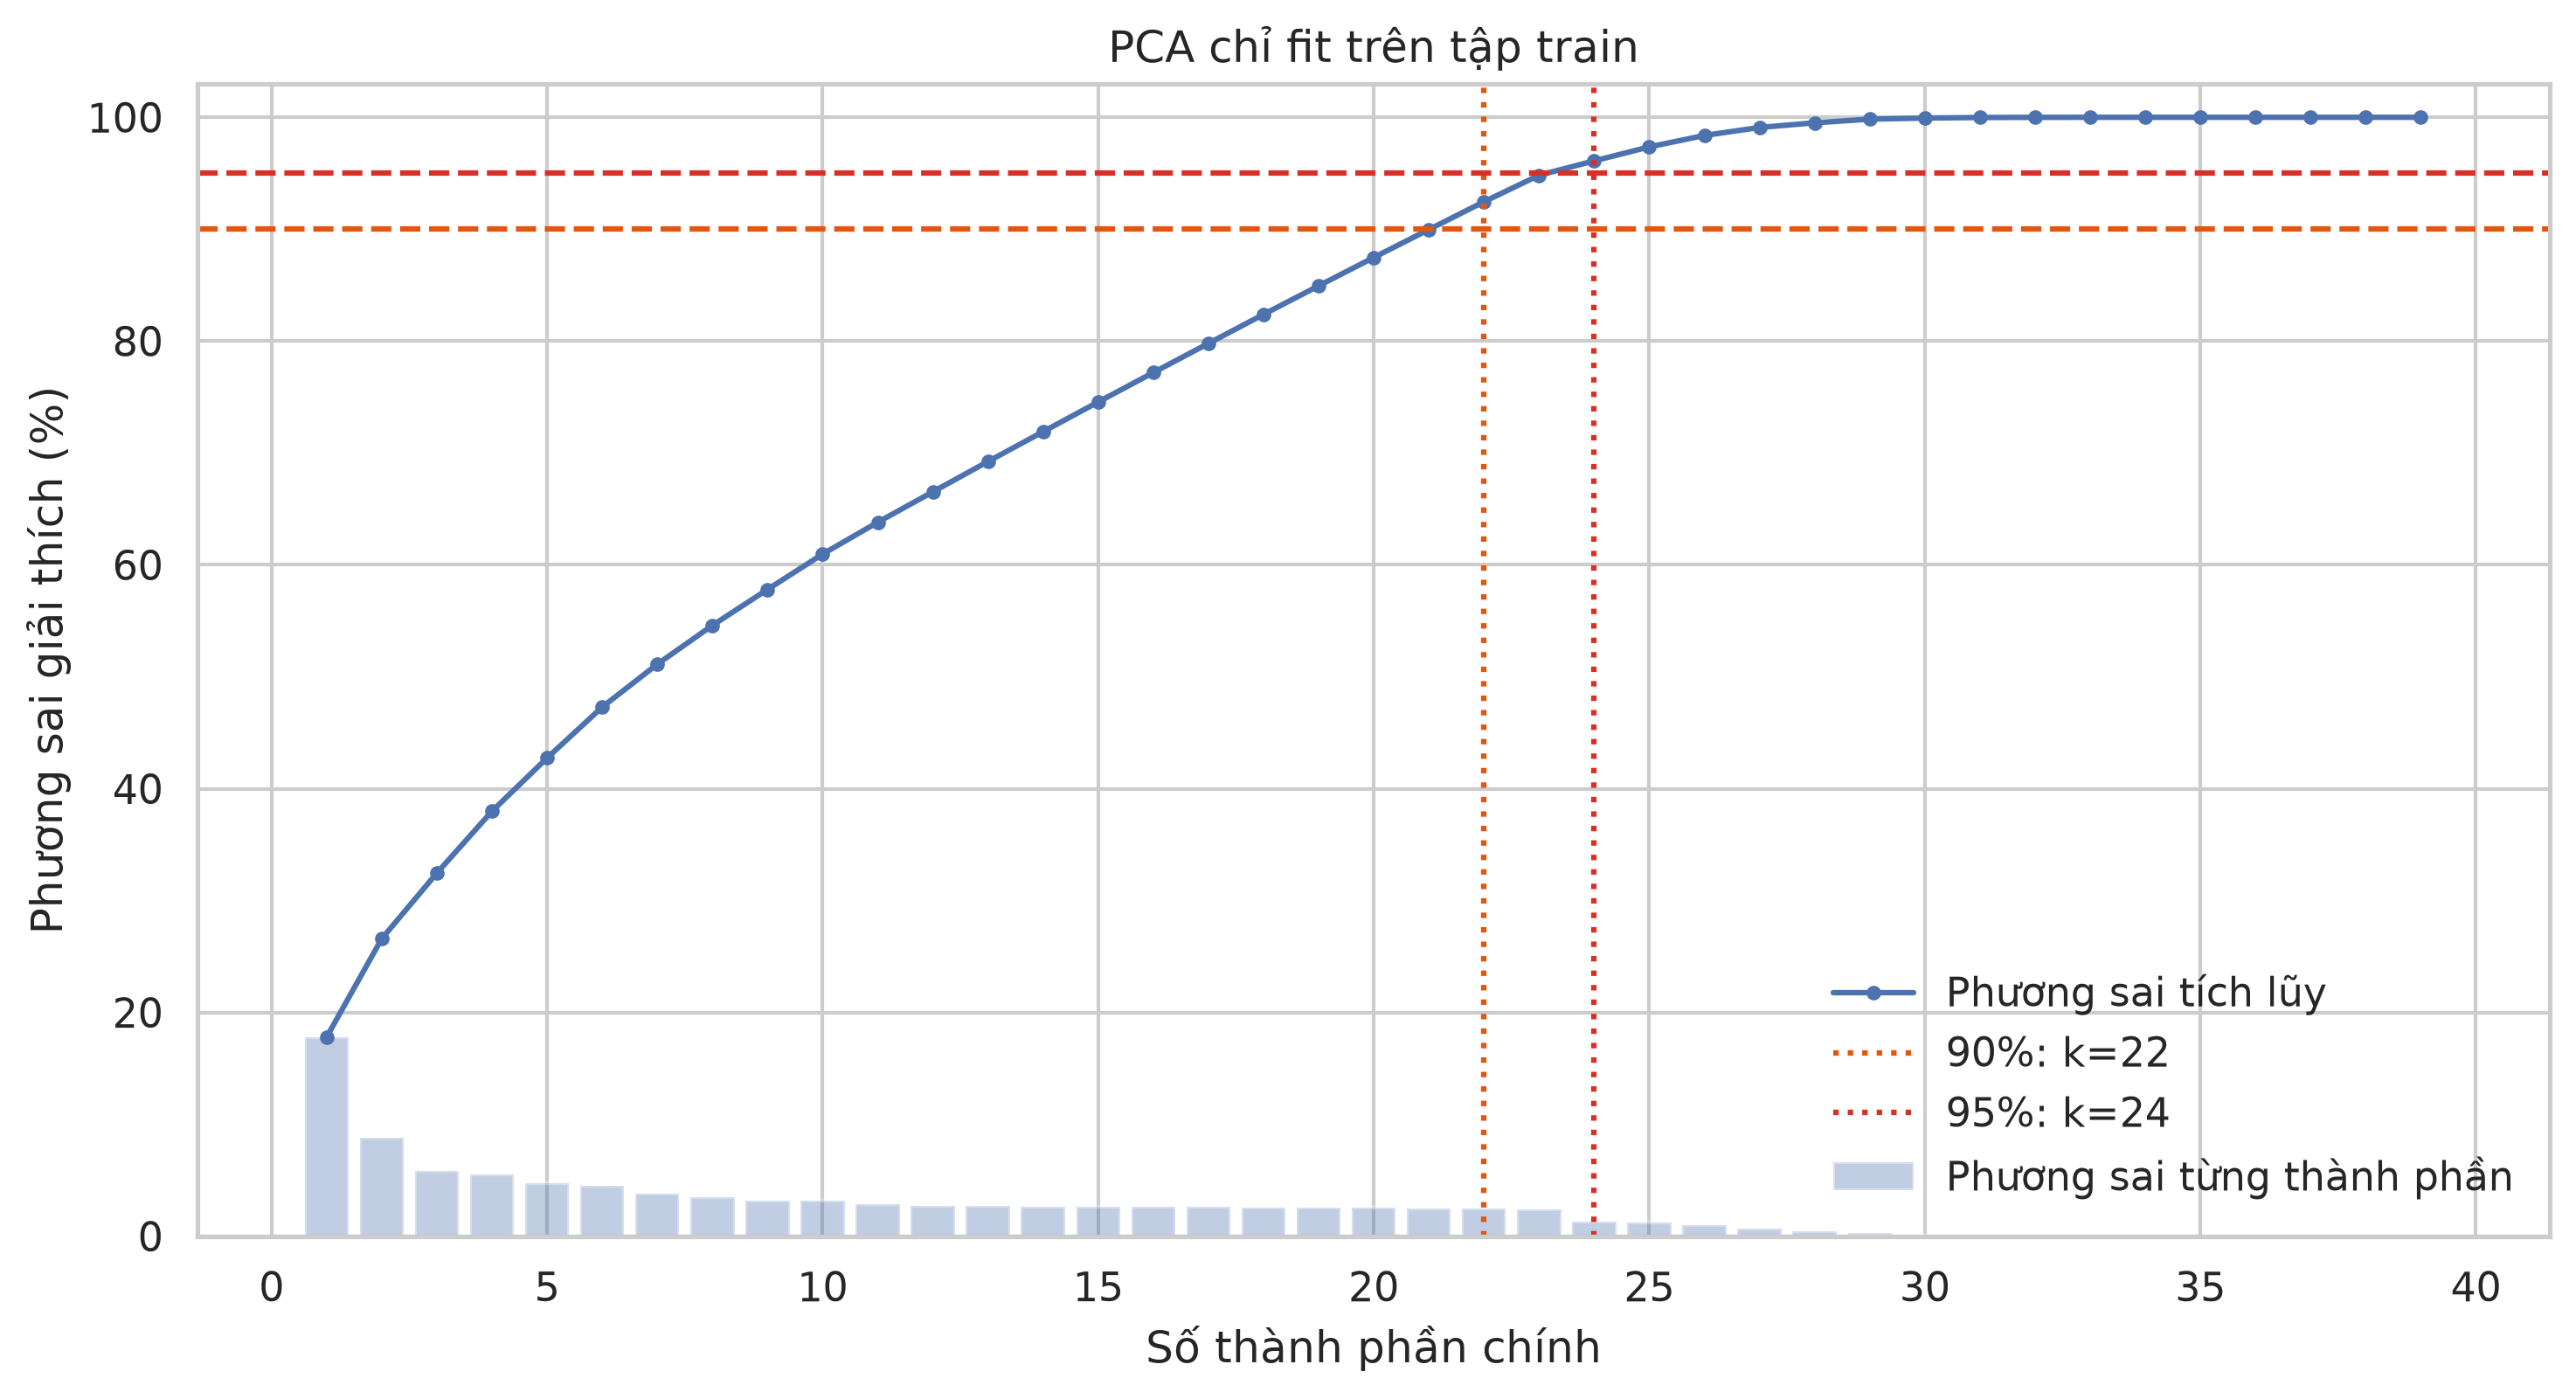
\includegraphics[width=0.85\textwidth]{group7_pca_scree_plot.png}
  \caption{Đường phương sai giải thích tích lũy của PCA fit trên train.}
  \label{fig:pca}
\end{figure}

\section{Mô hình truyền thống}

\subsection{Logistic Regression}

Mô hình ước lượng xác suất lớp dương bằng hàm sigmoid
\[
  P(y=1\mid \mathbf{x})=\sigma(\mathbf{w}^{\top}\mathbf{x}+b)
  =\frac{1}{1+\exp[-(\mathbf{w}^{\top}\mathbf{x}+b)]}.
\]
Regularization điều khiển bởi $C$ giúp cân bằng độ khớp và độ phức tạp. Logistic Regression là baseline nhanh, xác suất đầu ra trực tiếp và hệ số có thể diễn giải.

\subsection{Random Forest}

Random Forest kết hợp nhiều cây quyết định được xây dựng từ bootstrap sample và tập con đặc trưng ngẫu nhiên~[4]. Xác suất cuối là trung bình xác suất các cây. Mô hình phù hợp với quan hệ phi tuyến và tương tác, nhưng impurity importance có thể thiên lệch và mô hình lớn hơn Logistic Regression.

\section{Không gian cấu hình truyền thống}

Tổng cộng 24 candidate được đánh giá: 18 Logistic Regression và 6 Random Forest.

\begin{table}[H]
\centering
\caption{Không gian thí nghiệm truyền thống}\label{tab:traditional-search}
\begin{tabularx}{\textwidth}{l X X r}
\toprule
\textbf{Mô hình} & \textbf{Biểu diễn} & \textbf{Siêu tham số} & \textbf{Số candidate} \\
\midrule
Logistic Regression & Standard, PCA90, PCA95 & $C\in\{0{,}1;1;10\}$; \code{class\_weight}$\in\{$None, balanced$\}$ & 18 \\
Random Forest & Standard, PCA95 & 3 bộ cấu hình: 250--300 cây; depth 8, 12 hoặc không giới hạn; leaf 2, 3, 5; sqrt hoặc 0,7 số đặc trưng & 6 \\
\bottomrule
\end{tabularx}
\end{table}

MinMaxScaler với \code{feature\_range=(0,1)} cũng được hiện thực và xuất đặc trưng để chứng minh khả năng cấu hình pipeline. Search chính dùng Standard/PCA vì Standard phù hợp với regularization của Logistic Regression, còn PCA được fit trên dữ liệu đã chuẩn hóa. Random Forest không cần scaling về mặt lý thuyết; biểu diễn Standard ở đây giữ cùng ma trận đặc trưng và không thay đổi thứ tự trong từng cột.

\section{Chỉ số đánh giá và chọn ngưỡng}

Với $TP,TN,FP,FN$, các chỉ số threshold-dependent là:

\[
  \mathrm{Accuracy}=\frac{TP+TN}{TP+TN+FP+FN},\qquad
  \mathrm{Precision}=\frac{TP}{TP+FP},\qquad
  \mathrm{Recall}=\frac{TP}{TP+FN}.
\]
\[
  \mathrm{Specificity}=\frac{TN}{TN+FP},\qquad
  F_1=\frac{2\,\mathrm{Precision}\,\mathrm{Recall}}
  {\mathrm{Precision}+\mathrm{Recall}},\qquad
  \mathrm{Balanced\ Accuracy}=\frac{\mathrm{Recall}+\mathrm{Specificity}}{2}.
\]

ROC-AUC và PR-AUC đánh giá xếp hạng xác suất trên toàn bộ threshold. PR-AUC validation là tiêu chí chọn candidate chính vì lớp dương chỉ chiếm khoảng 25\%. Sau khi chọn candidate, threshold tối đa hóa F1 validation được khóa. Việc chọn threshold riêng giúp tránh mặc định 0,5 không phù hợp khi dùng class weight và dữ liệu lệch lớp.

% =============================================================================
\chapter{Thí nghiệm học máy truyền thống}
% =============================================================================

\section{Môi trường và khả năng tái lập}

Thí nghiệm sử dụng Python, NumPy, pandas, scikit-learn và seed 42. Metadata của lần chạy đã lưu ghi nhận Python 3.14.7, NumPy 2.5.4, pandas 3.1.0 và scikit-learn 1.9.1. Mã sử dụng API tương thích scikit-learn~[3]; yêu cầu tối thiểu được ghi trong \code{requirements.txt}. Split index, preprocessor, cấu hình JSON, feature array và model cuối đều được lưu để kiểm toán.

\section{Kết quả chọn cấu hình trên validation}

\begin{table}[H]
\centering
\caption{Candidate tốt nhất theo từng mô hình và biểu diễn trên validation}\label{tab:validation-best}
\resizebox{\textwidth}{!}{%
\begin{tabular}{lllrrrrl}
\toprule
\textbf{Mô hình} & \textbf{Biểu diễn} & \textbf{Candidate} & \textbf{PR-AUC} & \textbf{ROC-AUC} & \textbf{F1} & \textbf{Threshold} & \textbf{Cấu hình rút gọn} \\
\midrule
Logistic & Standard & LR-06 & \best{0,5262} & \best{0,7830} & \best{0,5918} & 0,5182 & $C=10$, balanced \\
Logistic & PCA90 & LR-07 & 0,5044 & 0,7594 & 0,5465 & 0,3087 & $C=0{,}1$, no weight \\
Logistic & PCA95 & LR-13 & 0,5102 & 0,7615 & 0,5446 & 0,3105 & $C=0{,}1$, no weight \\
Random Forest & Standard & RF-01 & \best{0,5372} & \best{0,7925} & \best{0,6204} & 0,6148 & 250 trees, depth 8, balanced \\
Random Forest & PCA95 & RF-06 & 0,5143 & 0,7693 & 0,5811 & 0,4381 & 300 trees, depth none, balanced subsample \\
\bottomrule
\end{tabular}}
\end{table}

PCA làm giảm hiệu năng của cả hai thuật toán. Đây là bằng chứng rằng phần phương sai bị loại tuy nhỏ nhưng có thể chứa tín hiệu dự đoán lớp dương, và phép chiếu tuyến tính làm mất cấu trúc cục bộ hữu ích cho cây. Standard 39 chiều được chọn cho cả hai mô hình. Candidate Logistic cuối dùng $C=10$, \code{class\_weight=balanced}; Random Forest dùng 250 cây, depth 8, leaf tối thiểu 2, \code{max\_features=sqrt} và \code{class\_weight=balanced}.

\section{Kết quả test khóa kín}

\begin{table}[H]
\centering
\caption{Kết quả hai mô hình truyền thống trên test}\label{tab:traditional-test}
\resizebox{\textwidth}{!}{%
\begin{tabular}{lrrrrrrrr}
\toprule
\textbf{Mô hình} & \textbf{Acc.} & \textbf{Bal. Acc.} & \textbf{Precision} & \textbf{Recall} & \textbf{Specificity} & \textbf{F1} & \textbf{ROC-AUC} & \textbf{PR-AUC} \\
\midrule
Logistic Regression & 0,7610 & 0,7644 & 0,5139 & \best{0,7713} & 0,7575 & 0,6168 & 0,7963 & 0,5288 \\
Random Forest & \best{0,7947} & \best{0,7725} & \best{0,5692} & 0,7280 & \best{0,8169} & \best{0,6389} & \best{0,8120} & \best{0,5414} \\
\bottomrule
\end{tabular}}
\end{table}

Confusion matrix của Logistic Regression là $TN=1634$, $FP=523$, $FN=164$, $TP=553$; Random Forest là $TN=1762$, $FP=395$, $FN=195$, $TP=522$. Logistic Regression phát hiện thêm 31 trường hợp dương nhưng tạo thêm 128 false positive. Random Forest cân bằng tốt hơn, tăng F1 khoảng 0,0221 và PR-AUC khoảng 0,0126 so với Logistic Regression.

\begin{figure}[H]
  \centering
  \begin{subfigure}[t]{0.49\textwidth}
    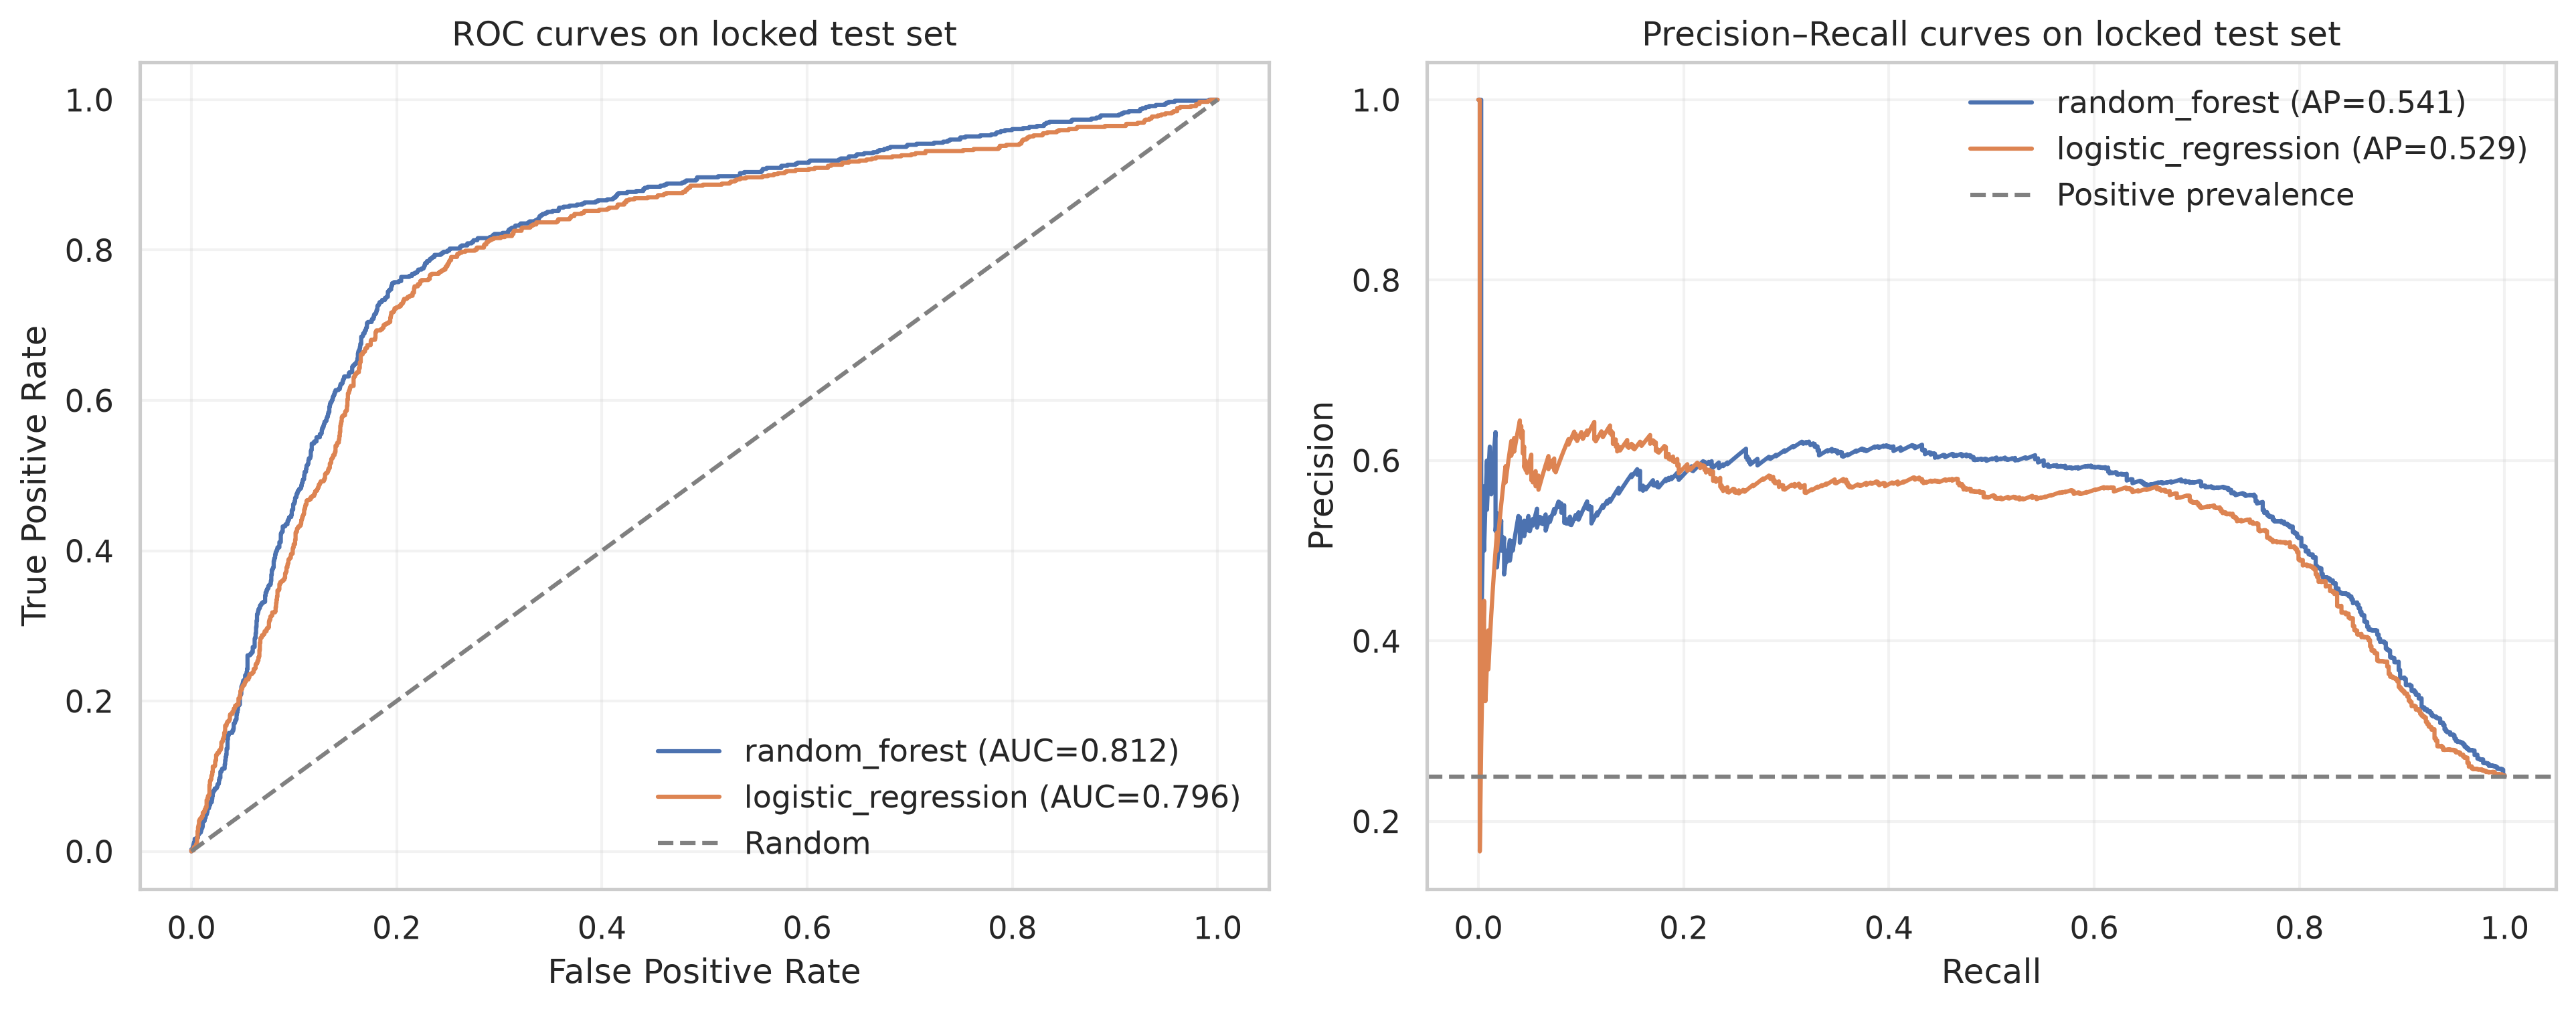
\includegraphics[width=\textwidth]{model_roc_pr_curves.png}
    \caption{Đường ROC và Precision--Recall.}
  \end{subfigure}
  \hfill
  \begin{subfigure}[t]{0.49\textwidth}
    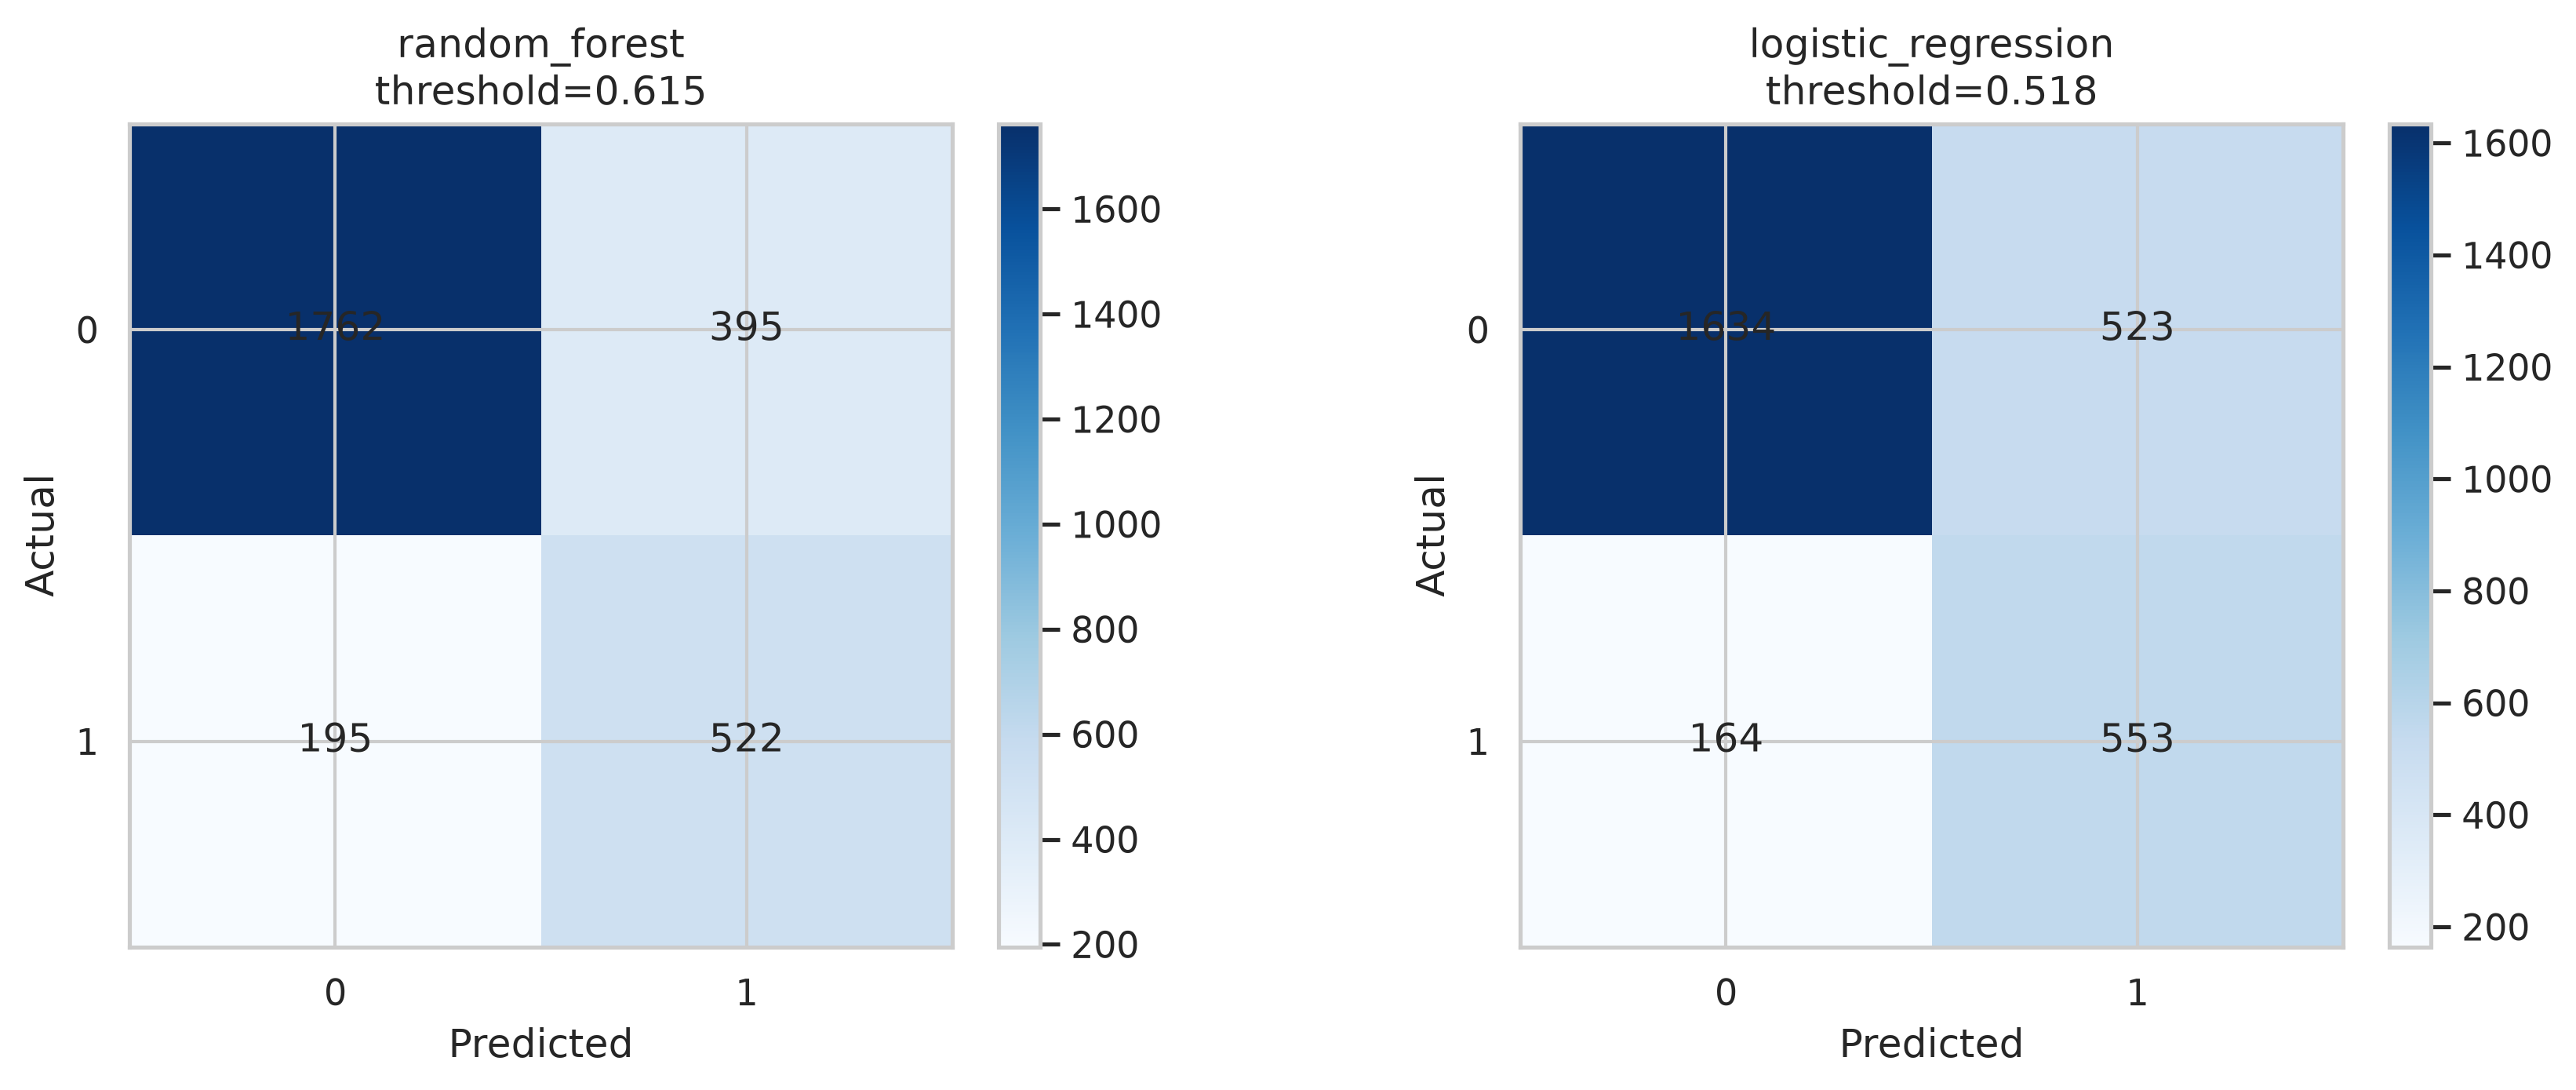
\includegraphics[width=\textwidth]{model_confusion_matrices.png}
    \caption{Confusion matrix tại threshold đã khóa.}
  \end{subfigure}
  \caption{Đánh giá hai mô hình truyền thống trên test.}
  \label{fig:traditional-test}
\end{figure}

\section{Diễn giải đặc trưng}

Hai mô hình cùng xem \code{city\_development\_index}, bình phương của nó và tương tác với kinh nghiệm là các tín hiệu quan trọng. Đối với Random Forest, ba importance đầu lần lượt là 0,2103; 0,2019; 0,0676. \code{company\_size\_isna} đứng thứ tư (0,0659), củng cố kết luận EDA rằng trạng thái thiếu thông tin công ty có giá trị dự đoán. \code{profile\_missing\_count} đứng thứ sáu (0,0515).

Hệ số Logistic Regression của \code{city\_development\_index} và bình phương có dấu trái ngược, phản ánh quan hệ cong thay vì đơn điệu. Các hệ số này được tính trên đặc trưng đã chuẩn hóa; không nên diễn giải như tác động nhân quả. Importance của Random Forest cũng là impurity-based và chỉ phản ánh đóng góp nội bộ của mô hình.

% =============================================================================
\chapter{Mở rộng học sâu với ResNet và TabM}
% =============================================================================

\section{Lý do lựa chọn}

Nhánh học sâu dùng hai kiến trúc bổ trợ. ResNet là residual MLP mạnh cho dữ liệu bảng: các block học hiệu chỉnh trên một biểu diễn chung và skip connection giúp tối ưu mạng sâu ổn định hơn~[5]. TabM là ensemble MLP hiệu quả tham số; các member chia sẻ ma trận trọng số nhưng có rank-one adapter riêng, sau đó trung bình xác suất khi suy luận~[7]. Mục tiêu không phải giả định deep learning luôn vượt mô hình cây, mà đánh giá công bằng khả năng học embedding và tương tác trên cùng split.

\section{Tiền xử lý và kiến trúc}

Nhánh deep sử dụng mười trường categorical: \code{city}, \code{gender}, \code{relevent\_experience}, \code{enrolled\_university}, \code{education\_level}, \code{major\_discipline}, \code{experience}, \code{company\_size}, \code{company\_type}, \code{last\_new\_job}. ID 0 dành cho giá trị chưa thấy và ID 1 dành cho missing; vocabulary chỉ học trên train. Mười ba numerical/engineered features được điền median và z-score bằng thống kê train.

Mỗi categorical field có embedding riêng. Các embedding được nối với vector số đã chuẩn hóa. ResNet chiếu vector này lên $d_{block}$ chiều rồi qua các residual block gồm LayerNorm, hai lớp tuyến tính, ReLU và dropout. TabM dùng các lớp tuyến tính BatchEnsemble: member $m$ điều chỉnh đầu vào/đầu ra bằng các vector tỉ lệ hạng một trong khi giữ trọng số lõi dùng chung. Mô hình tạo nhiều logit song song và lấy trung bình xác suất member khi suy luận.

\section{Huấn luyện và không gian cấu hình}

Ba candidate cho mỗi thuật toán được huấn luyện bằng AdamW, BCEWithLogitsLoss, cosine learning-rate schedule, gradient clipping 1,0 và batch size 512. Early stopping theo validation PR-AUC; ROC-AUC dùng phá hòa. Bảng dưới ghi candidate thắng của mỗi họ; toàn bộ sáu cấu hình nằm trong \code{configs/deep\_learning\_experiments.json}.

\begin{table}[H]
\centering
\caption{Cấu hình học sâu được khóa trên validation}\label{tab:deep-config}
\resizebox{\textwidth}{!}{%
\begin{tabular}{lrrrrrrrr}
\toprule
\textbf{Mô hình} & \textbf{Embed} & $d_{block}$ & \textbf{Blocks} & \textbf{Members} & \textbf{Dropout} & \textbf{LR} & \textbf{WD} & \textbf{Seed} \\
\midrule
ResNet & 16 & 256 & 3 & -- & 0,25 & $5\times10^{-4}$ & $3\times10^{-4}$ & 123 \\
TabM & 12 & 192 & 3 & 8 & 0,20 & $10^{-3}$ & $10^{-4}$ & 123 \\
\bottomrule
\end{tabular}}
\end{table}

Hai winner có tối đa 120 epoch và patience 18 nhưng cùng đạt validation tốt nhất ở epoch 7. ResNet có 838.833 tham số; TabM có 521.149 tham số với tám member nội bộ.

\section{Chọn checkpoint hoàn toàn trên validation}

ResNet và TabM được chọn độc lập theo validation PR-AUC, sau đó threshold tối đa hóa F1 validation được khóa riêng. ResNet winner đạt validation PR-AUC 0,5583, threshold 0,3254; TabM winner đạt 0,5561, threshold 0,4168. TabM đã là ensemble nội bộ, vì vậy không tạo thêm ensemble giữa các candidate hay giữa hai thuật toán.

\begin{figure}[H]
  \centering
  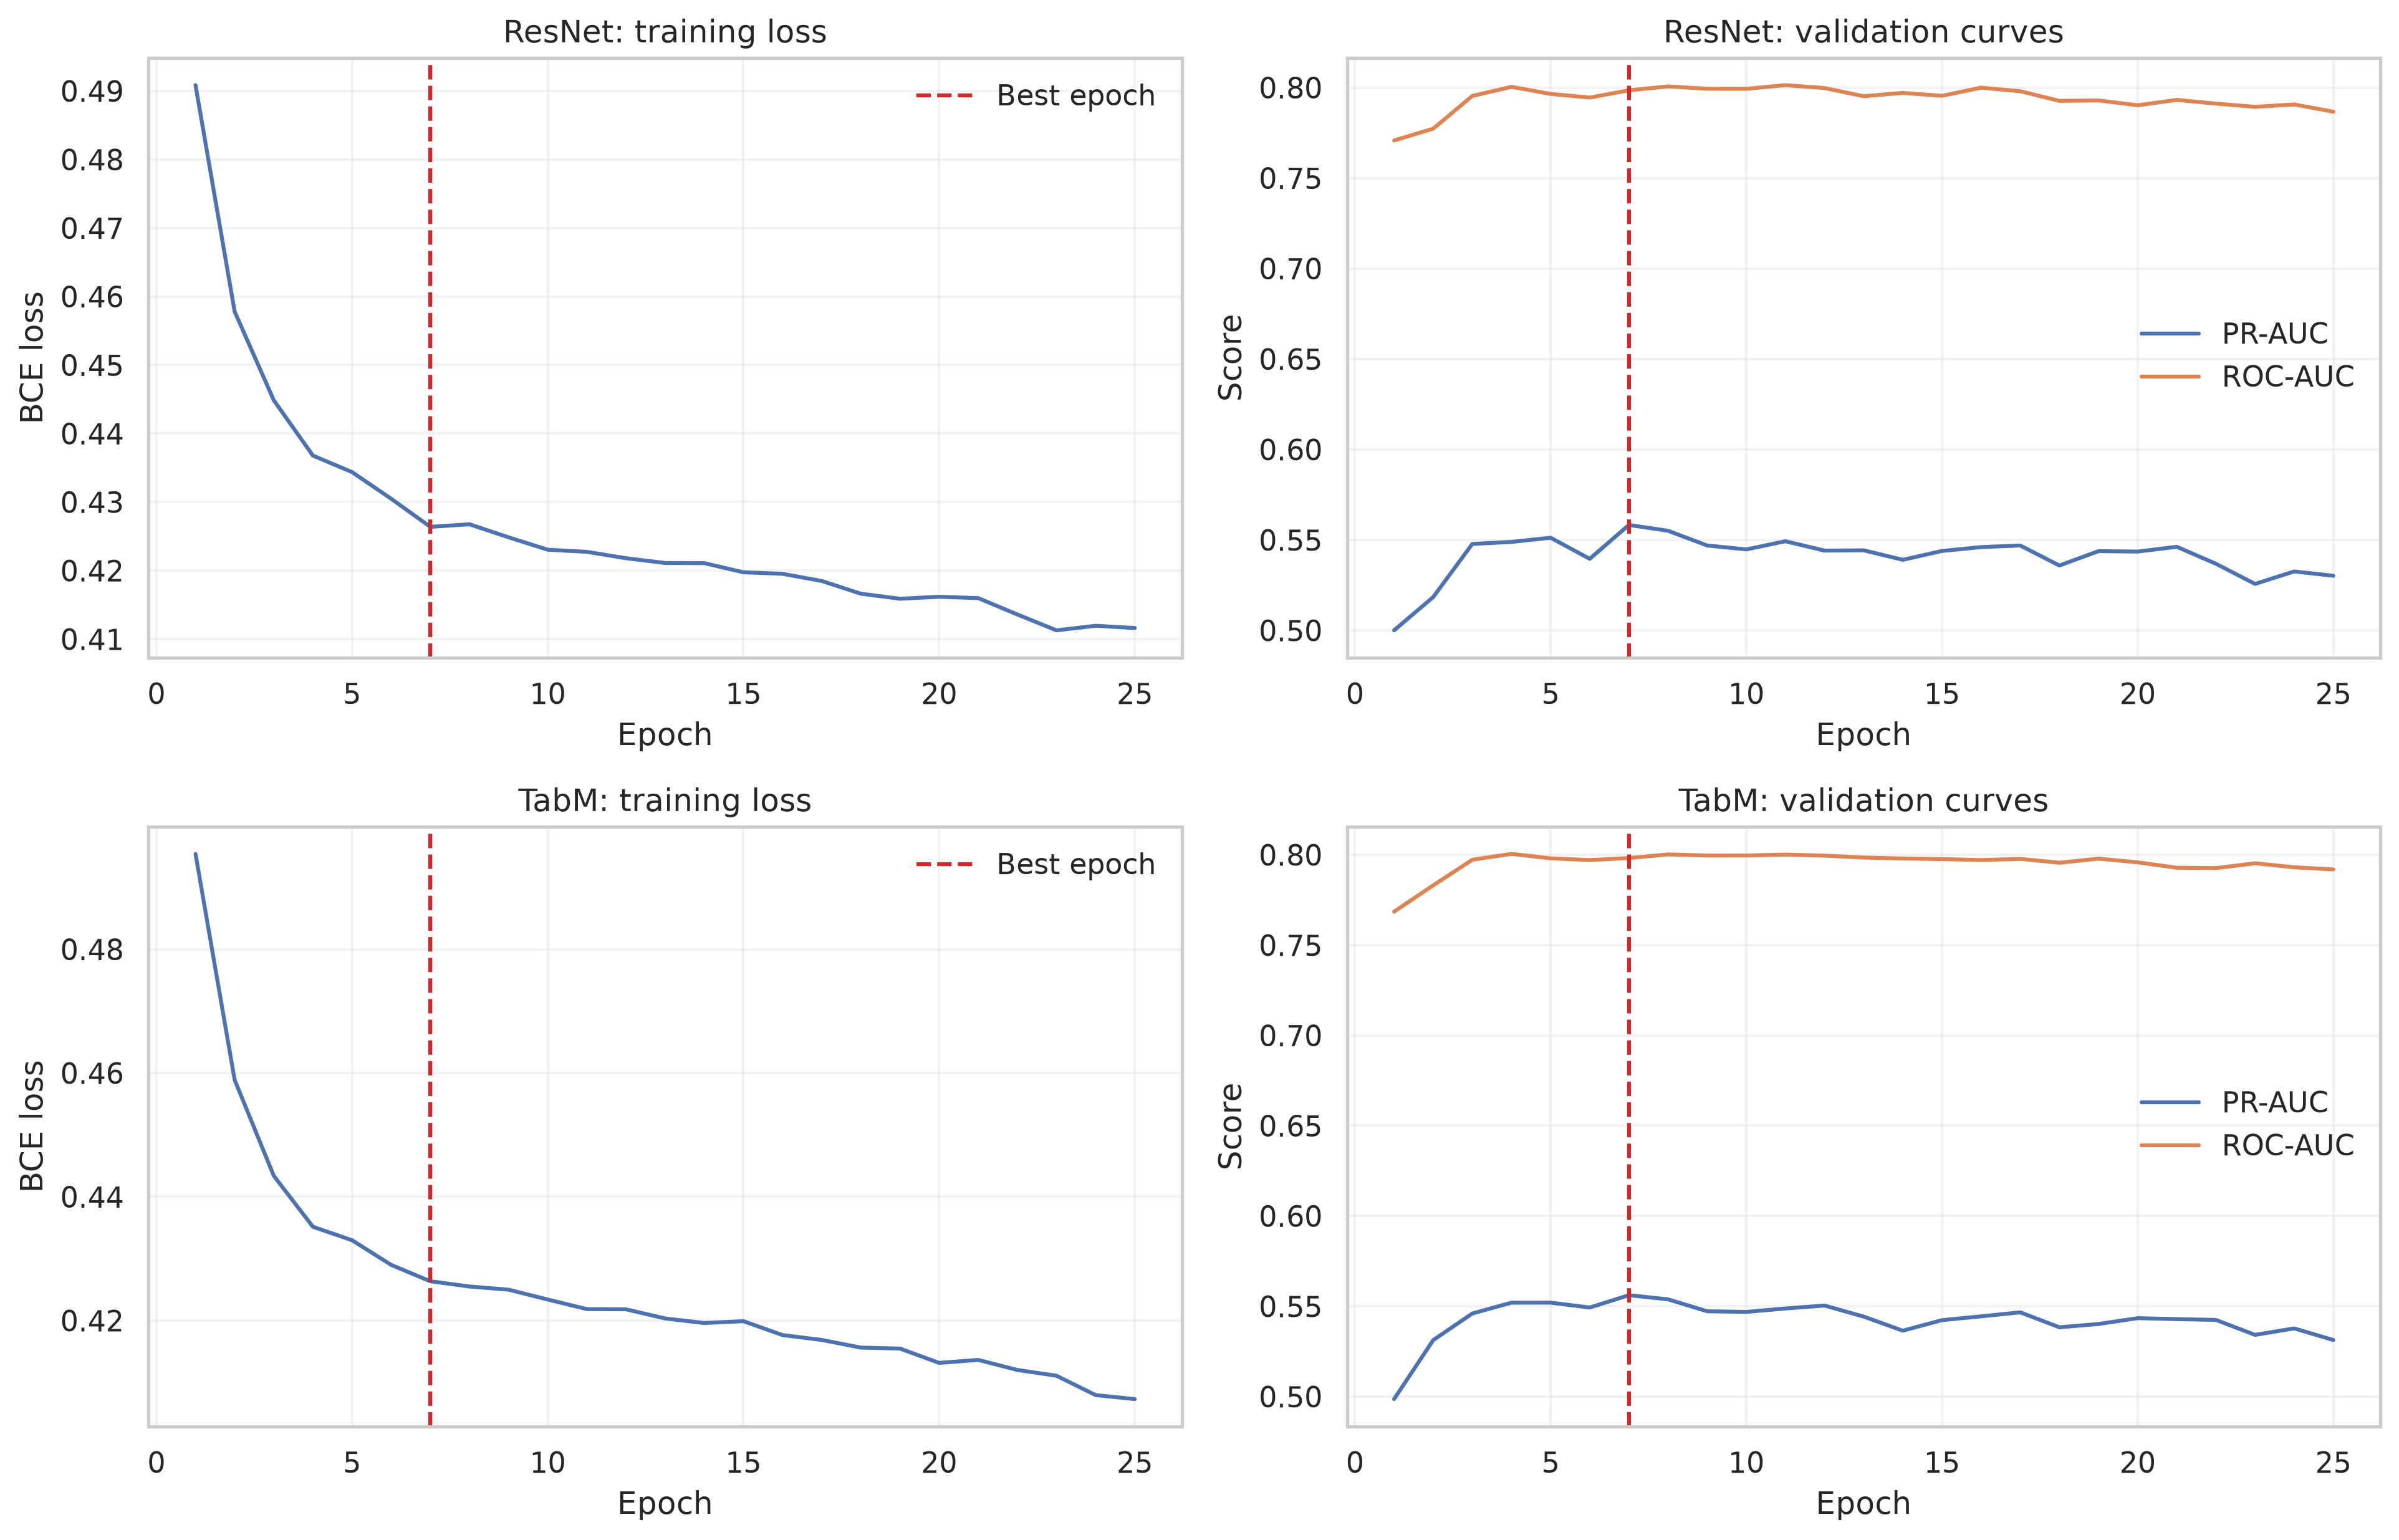
\includegraphics[width=0.98\textwidth]{deep_models_learning_curves.png}
  \caption{Learning curve của ResNet và TabM được chọn.}
  \label{fig:deep-learning-curves}
\end{figure}

\section{Kết quả deep learning trên test}

ResNet đạt $TN=1749$, $FP=408$, $FN=183$, $TP=534$; TabM đạt $TN=1759$, $FP=398$, $FN=189$, $TP=528$. Kết quả tổng hợp:

\begin{table}[H]
\centering
\caption{So sánh bốn thuật toán trên test khóa kín}\label{tab:all-test}
\resizebox{\textwidth}{!}{%
\begin{tabular}{lrrrrrrr}
\toprule
\textbf{Thuật toán} & \textbf{Accuracy} & \textbf{Bal. Acc.} & \textbf{Precision} & \textbf{Recall} & \textbf{F1} & \textbf{ROC-AUC} & \textbf{PR-AUC} \\
\midrule
Logistic Regression & 0,7610 & 0,7644 & 0,5139 & \best{0,7713} & 0,6168 & 0,7963 & 0,5288 \\
Random Forest & 0,7947 & 0,7725 & 0,5692 & 0,7280 & 0,6389 & \best{0,8120} & 0,5414 \\
ResNet & 0,7944 & \best{0,7778} & 0,5669 & 0,7448 & \best{0,6438} & 0,8087 & \best{0,5657} \\
TabM & \best{0,7958} & 0,7759 & \best{0,5702} & 0,7364 & 0,6427 & 0,8093 & 0,5576 \\
\bottomrule
\end{tabular}}
\end{table}

So với Random Forest, ResNet tăng PR-AUC 0,0243 và F1 0,0048; TabM tăng PR-AUC 0,0161 và F1 0,0038. Random Forest vẫn có ROC-AUC cao nhất; TabM có Accuracy/Precision cao nhất; Logistic Regression có Recall cao nhất. Không mô hình nào thắng mọi chỉ số và chênh lệch điểm đơn chưa đủ chứng minh khác biệt tổng quát.

\begin{figure}[H]
  \centering
  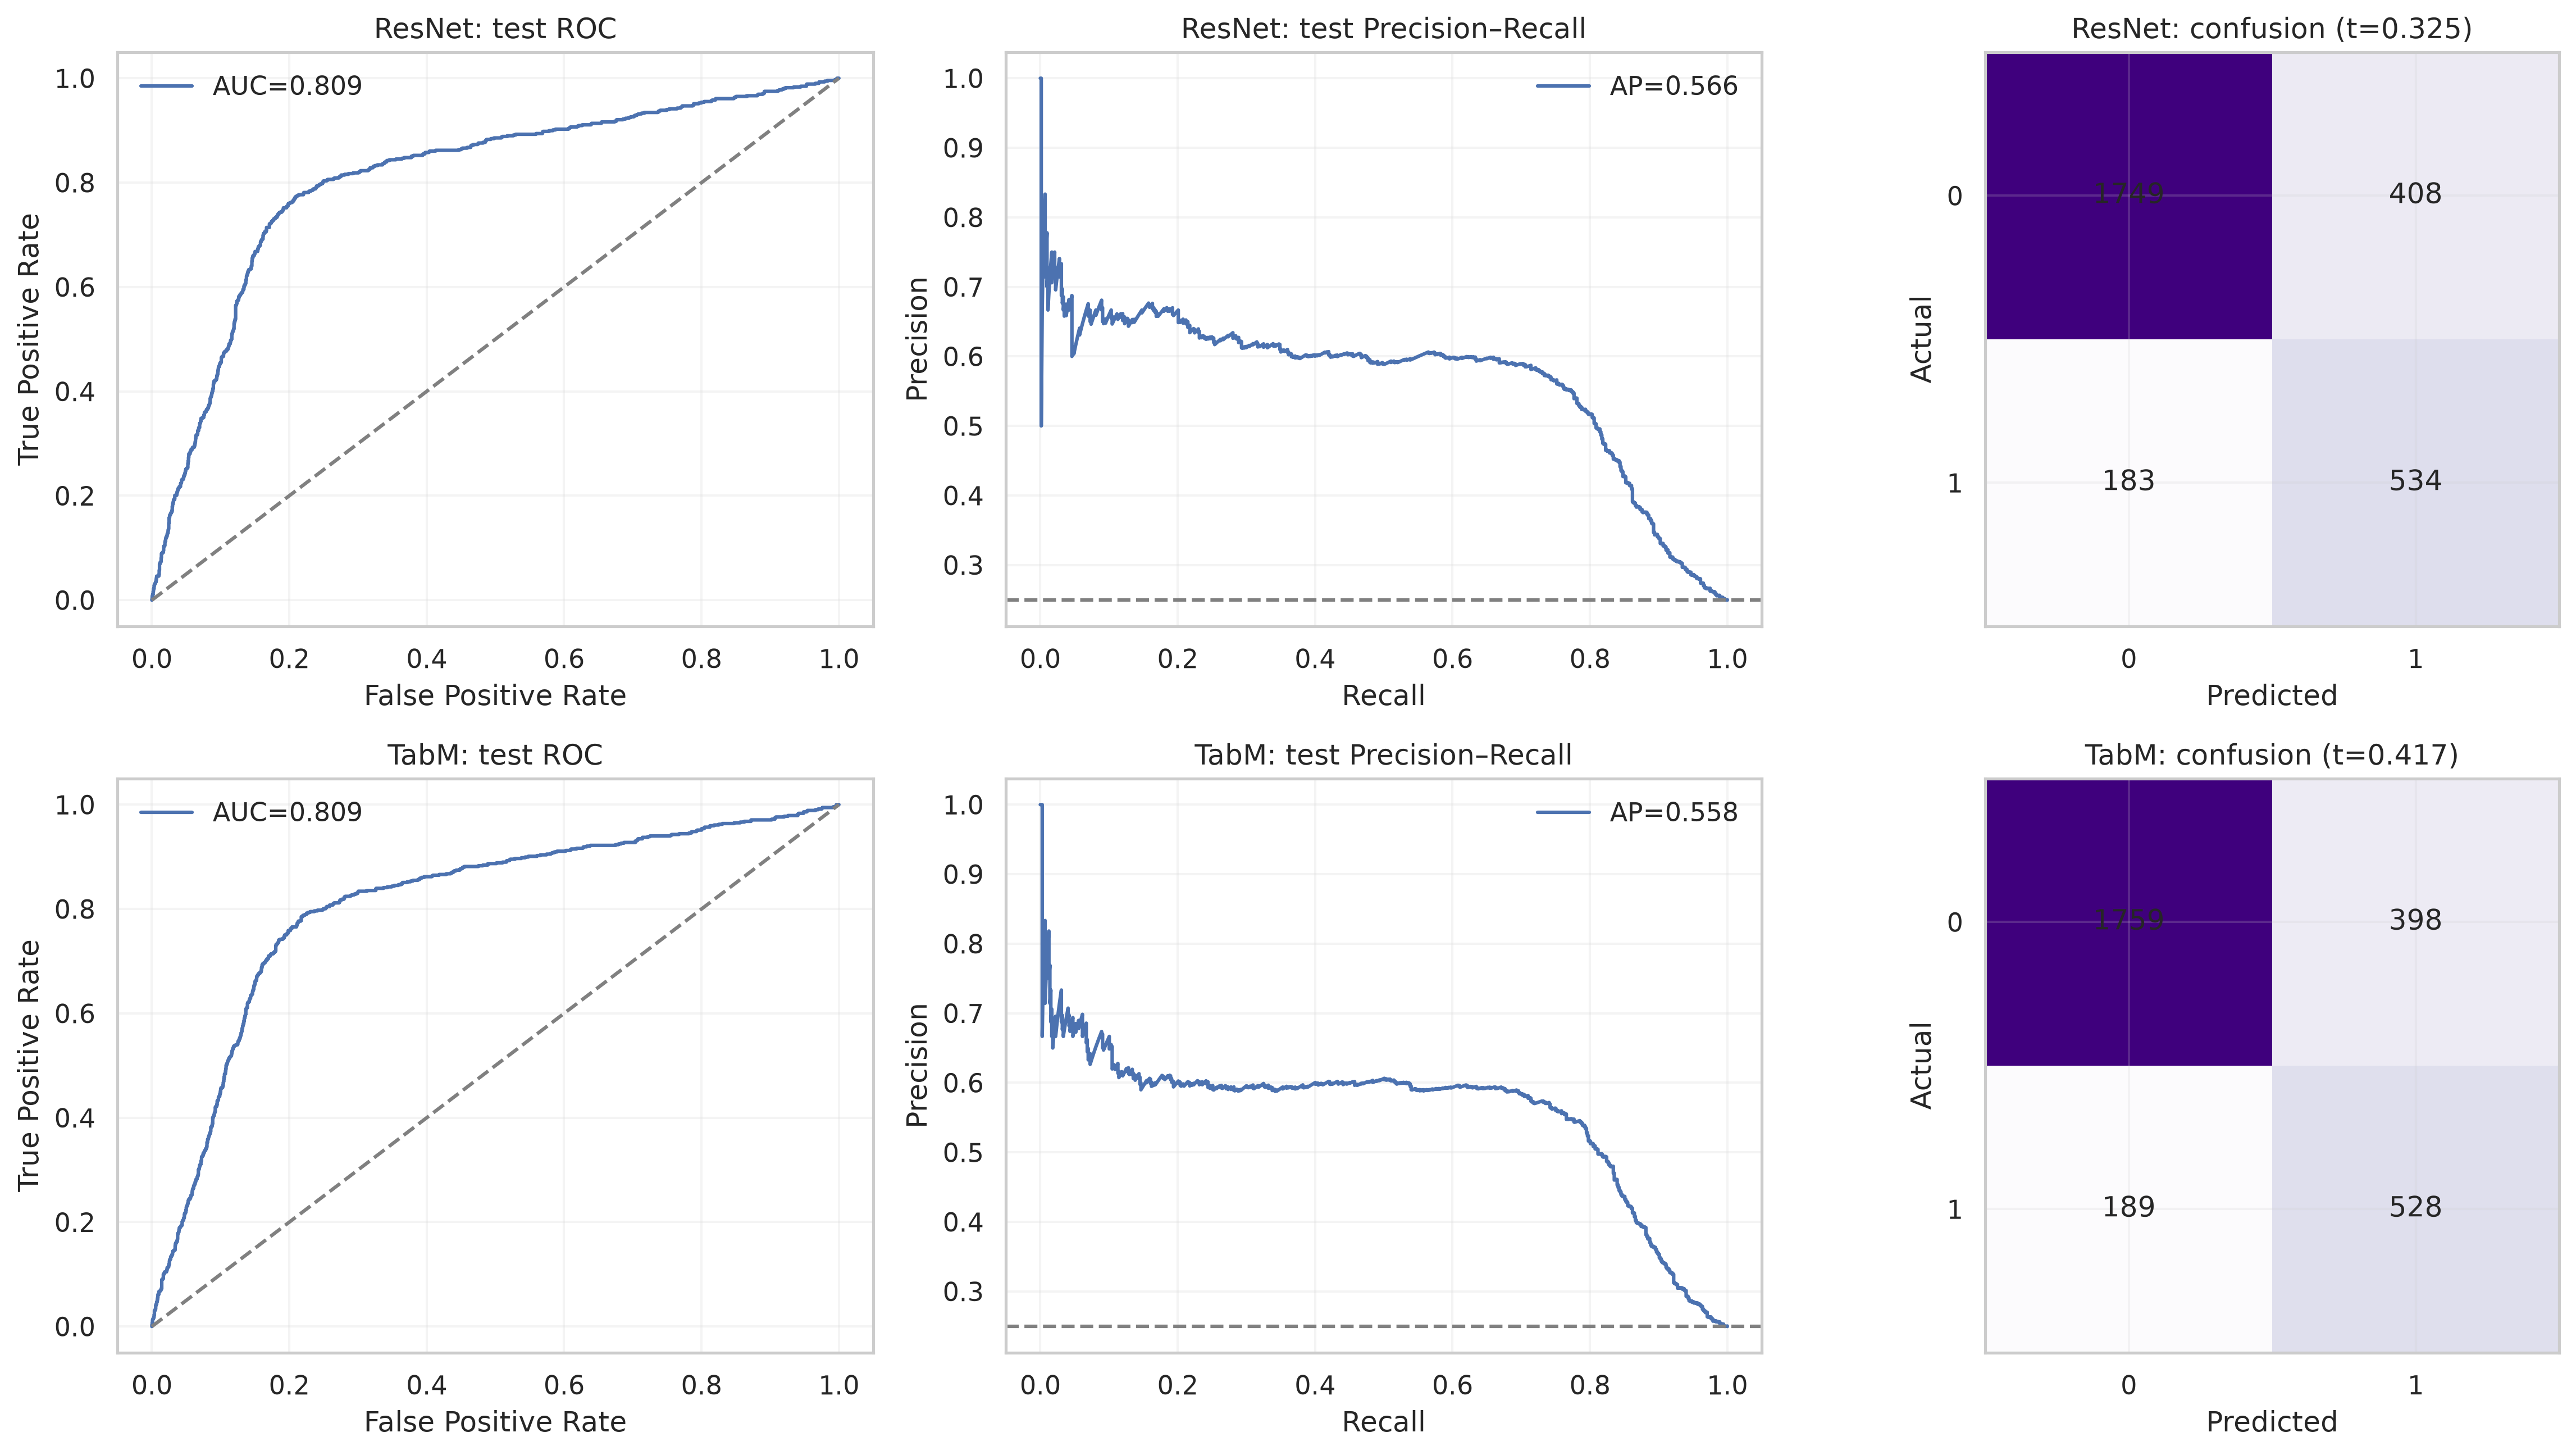
\includegraphics[width=0.98\textwidth]{deep_models_test_evaluation.png}
  \caption{ROC, Precision--Recall và confusion matrix của ResNet và TabM trên test.}
  \label{fig:deep-test}
\end{figure}

\begin{figure}[H]
  \centering
  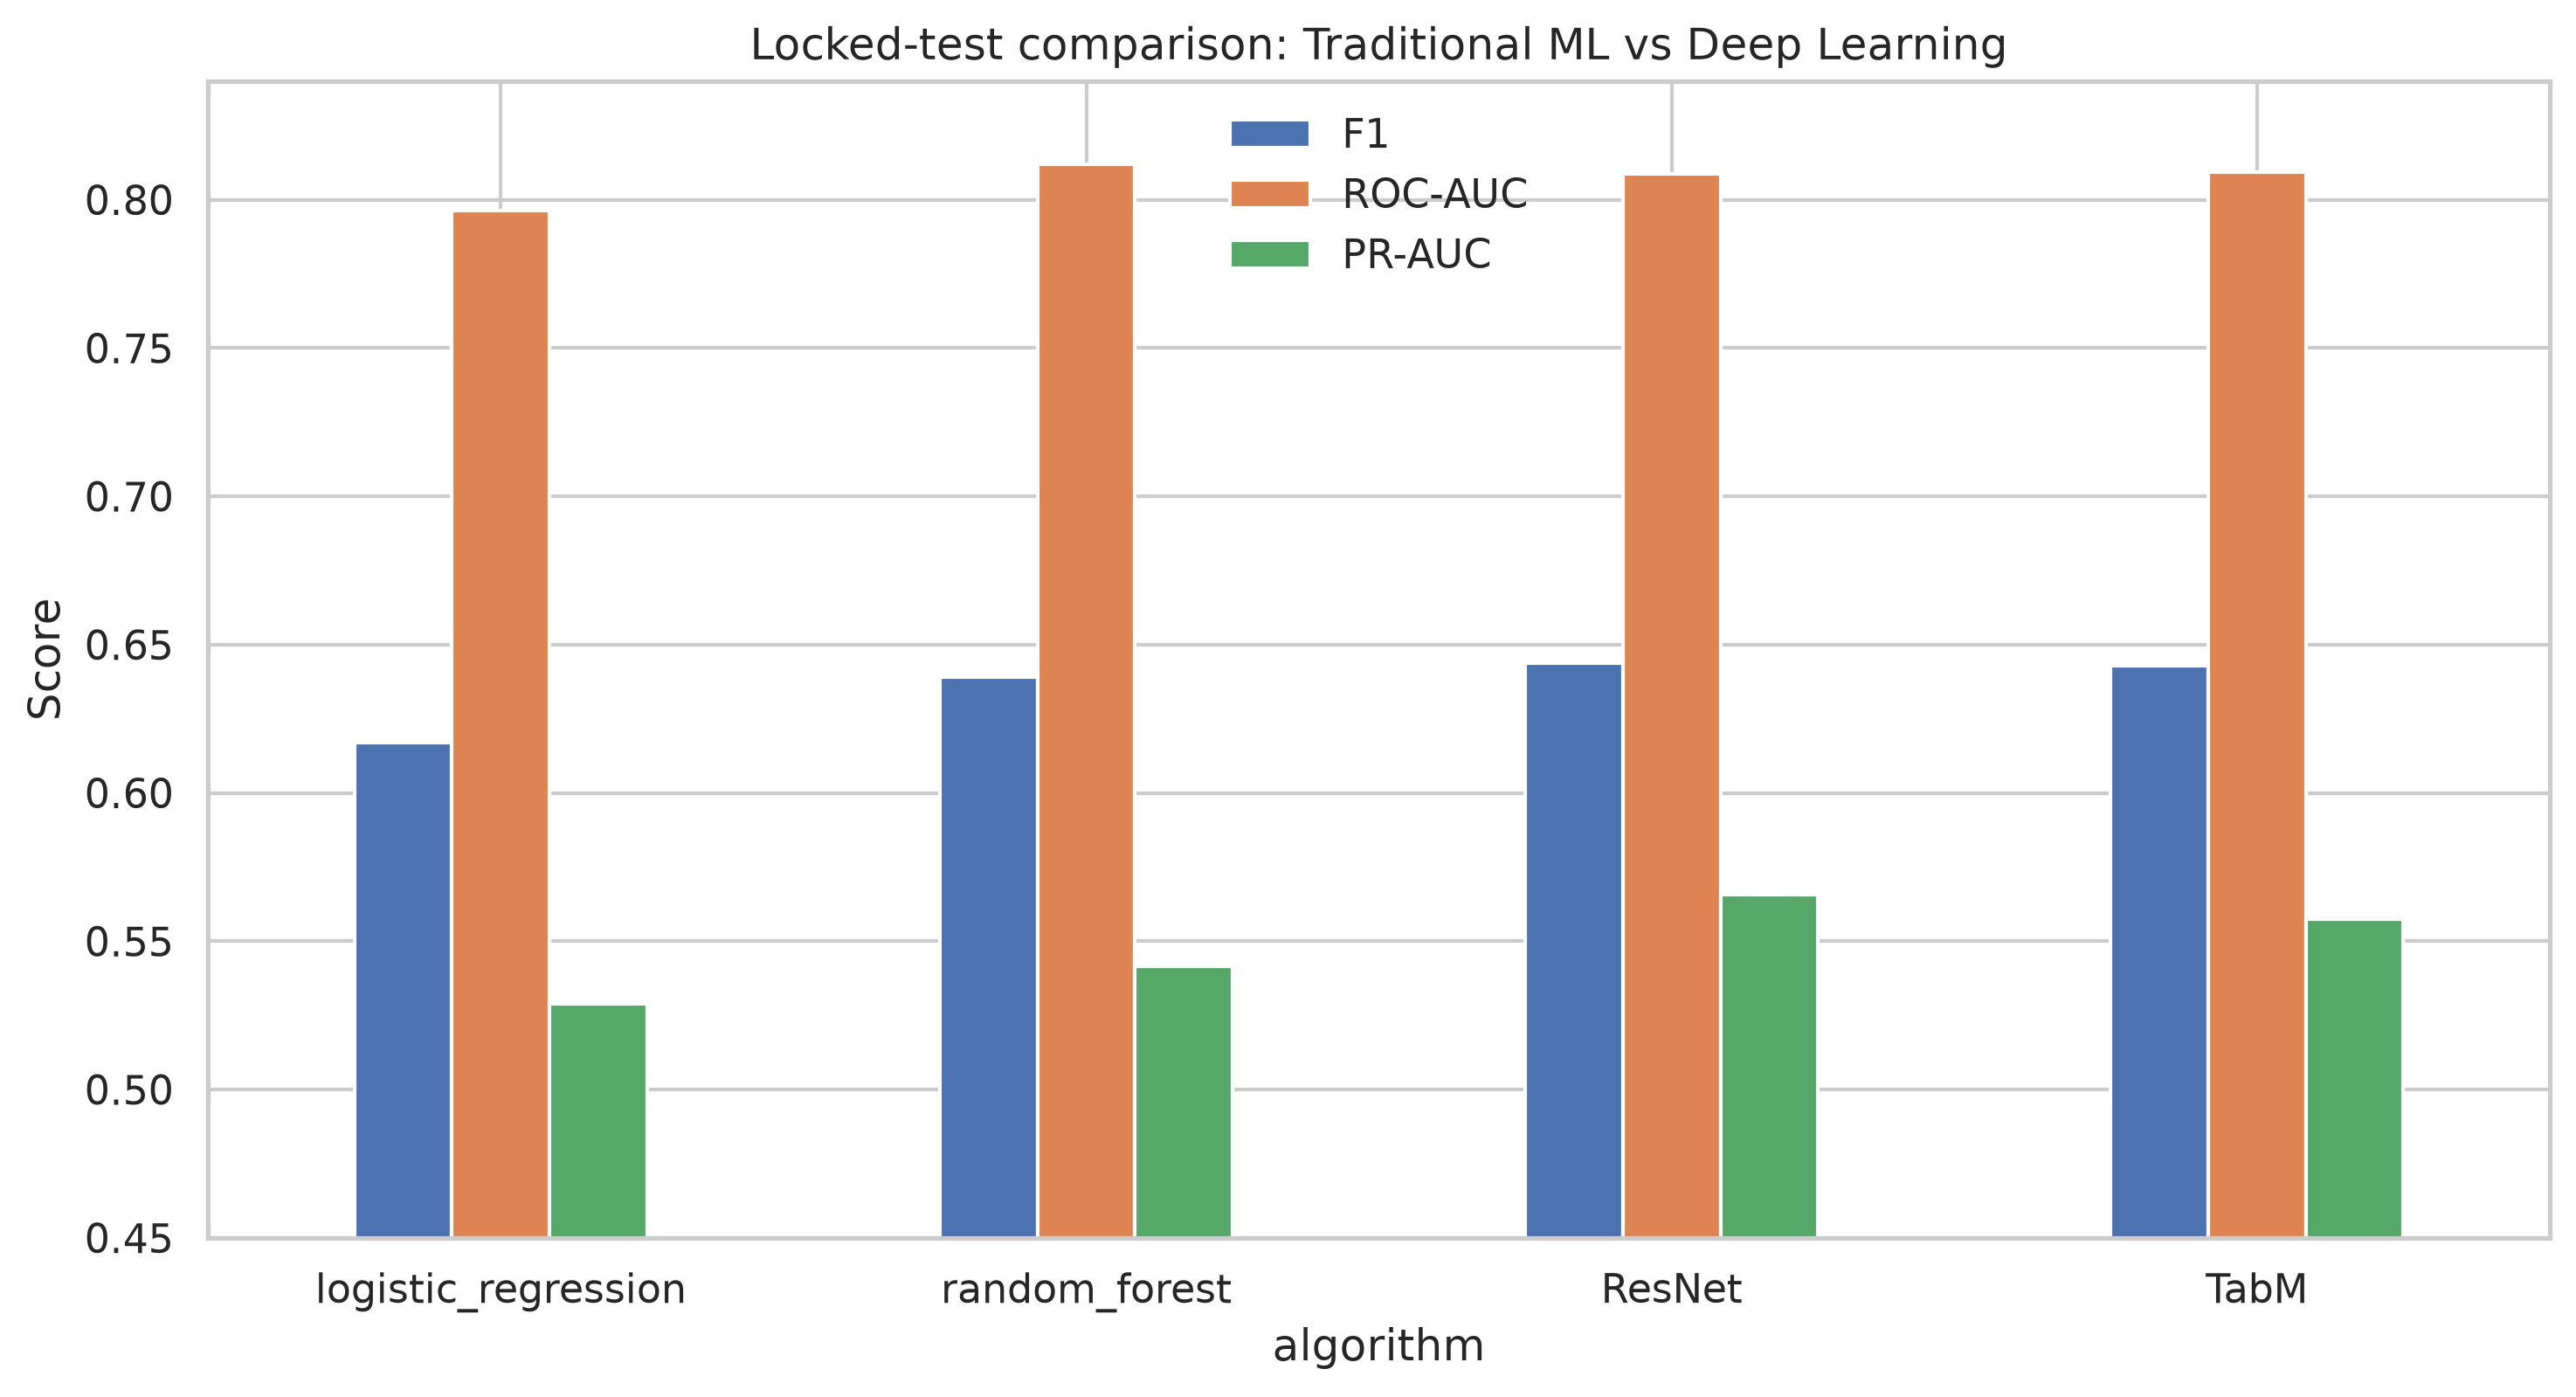
\includegraphics[width=0.90\textwidth]{all_models_metric_comparison.png}
  \caption{So sánh F1, ROC-AUC và PR-AUC của bốn thuật toán.}
  \label{fig:all-comparison}
\end{figure}

% =============================================================================
\chapter{Thảo luận}
% =============================================================================

\section{Trả lời câu hỏi nghiên cứu}

\textbf{Cấu hình truyền thống tốt nhất.} Standard 39 chiều tốt hơn PCA90/PCA95. Random Forest RF-01 là mô hình truyền thống mạnh nhất theo validation PR-AUC và tiếp tục dẫn đầu các mô hình truyền thống trên test.

\textbf{Vai trò của missingness và đặc trưng.} Missingness của thông tin công ty liên quan mạnh đến target; các cờ khuyết và tổng số trường thiếu xuất hiện trong top importance. Chỉ số phát triển thành phố và các biến tương tác với kinh nghiệm là nhóm tín hiệu nổi bật nhất.

\textbf{Lợi ích của học sâu.} ResNet đạt PR-AUC, F1 và Balanced Accuracy cao nhất; TabM đạt Accuracy/Precision cao nhất. Bootstrap cặp 2.000 lần cho chênh lệch ResNet--Random Forest cho khoảng PR-AUC 95\% xấp xỉ $[0{,}00001;0{,}04734]$, trong khi khoảng F1 là $[-0{,}00581;0{,}01613]$. Bằng chứng cải thiện xếp hạng lớp dương mạnh hơn bằng chứng cải thiện quyết định tại threshold.

\section{So sánh định tính}

\begin{table}[H]
\centering
\caption{Ưu điểm và hạn chế của các mô hình}\label{tab:qualitative}
\begin{tabularx}{\textwidth}{l X X}
\toprule
\textbf{Mô hình} & \textbf{Ưu điểm} & \textbf{Hạn chế} \\
\midrule
Logistic Regression & Rất nhanh; baseline minh bạch; Recall cao; hệ số có dấu. & Giả định tuyến tính trên log-odds; cần feature engineering; precision thấp hơn. \\
Random Forest & Phi tuyến; mạnh trên tabular; ít tuning; hiệu năng/chi phí tốt. & Model lớn hơn; impurity importance có thiên lệch; xác suất có thể cần calibration. \\
ResNet & Học embedding/tương tác; PR-AUC và F1 cao nhất. & Tốn thời gian hơn; nhạy seed; khó diễn giải; lợi ích F1 chưa chắc chắn. \\
TabM & Ensemble nội bộ hiệu quả tham số; Accuracy/Precision cao. & Kiến trúc phức tạp; lợi ích so với Random Forest nhỏ. \\
\bottomrule
\end{tabularx}
\end{table}

Candidate Logistic và Random Forest nhanh hơn đáng kể so với search học sâu trên CPU. Do đó, nếu ưu tiên độ đơn giản, latency huấn luyện và khả năng giải thích, Random Forest là lựa chọn thực dụng. Nếu khả năng xếp hạng lớp dương quan trọng và có tài nguyên, ResNet có lợi thế theo PR-AUC trên test hiện tại.

\section{Audit độ ổn định, calibration và fairness}

Repeated stratified 5-fold cross-validation ba lần trên train+validation, với cấu hình truyền thống đã khóa, cho Logistic Regression PR-AUC $0{,}5245\pm0{,}0115$ và Random Forest $0{,}5457\pm0{,}0148$. Thứ hạng này phù hợp với validation/test và cho thấy kết luận giữa hai baseline không phụ thuộc hoàn toàn vào một split.

Ablation validation cho Random Forest cho thấy bỏ engineered features làm F1 giảm từ 0,6204 xuống 0,6101; bỏ missing indicators làm PR-AUC giảm từ 0,5372 xuống 0,5295. Tuy nhiên biến thể bỏ cả hai đạt PR-AUC 0,5409, minh họa tương tác giữa nhóm đặc trưng và cảnh báo không diễn giải ablation đơn lẻ như tác động nhân quả.

\begin{figure}[H]
  \centering
  \begin{subfigure}[t]{0.49\textwidth}
    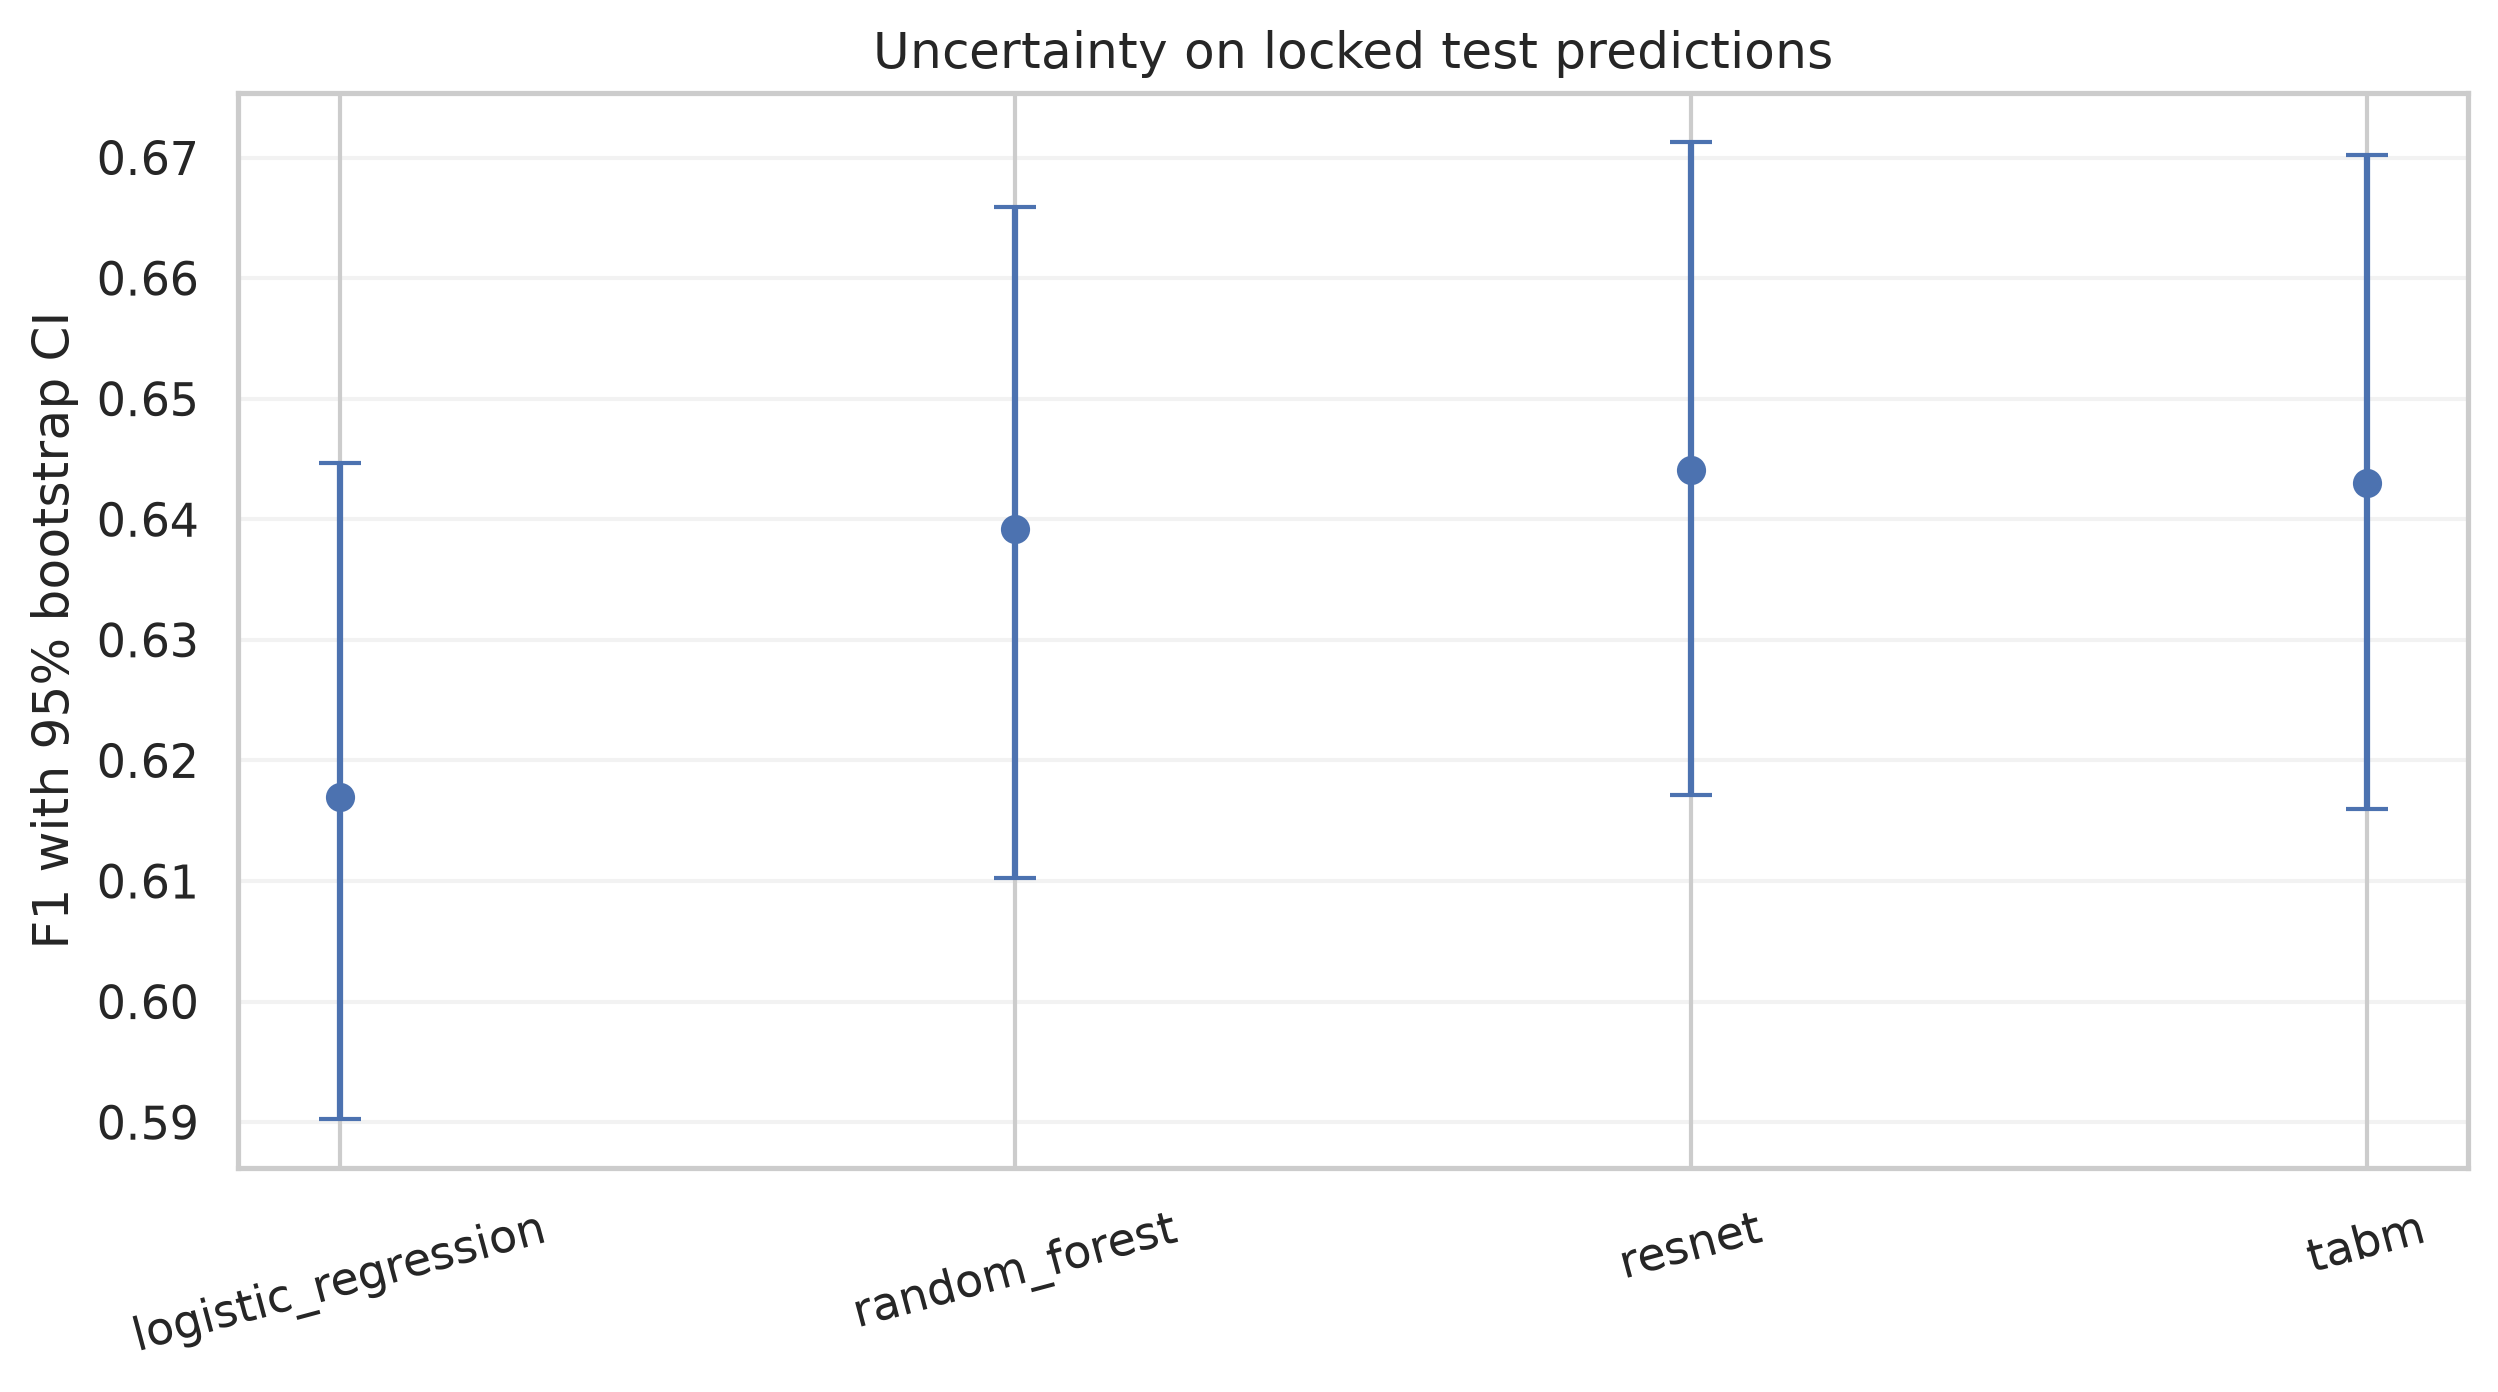
\includegraphics[width=\textwidth]{model_bootstrap_f1.png}
    \caption{Khoảng tin cậy bootstrap cho F1.}
  \end{subfigure}
  \hfill
  \begin{subfigure}[t]{0.49\textwidth}
    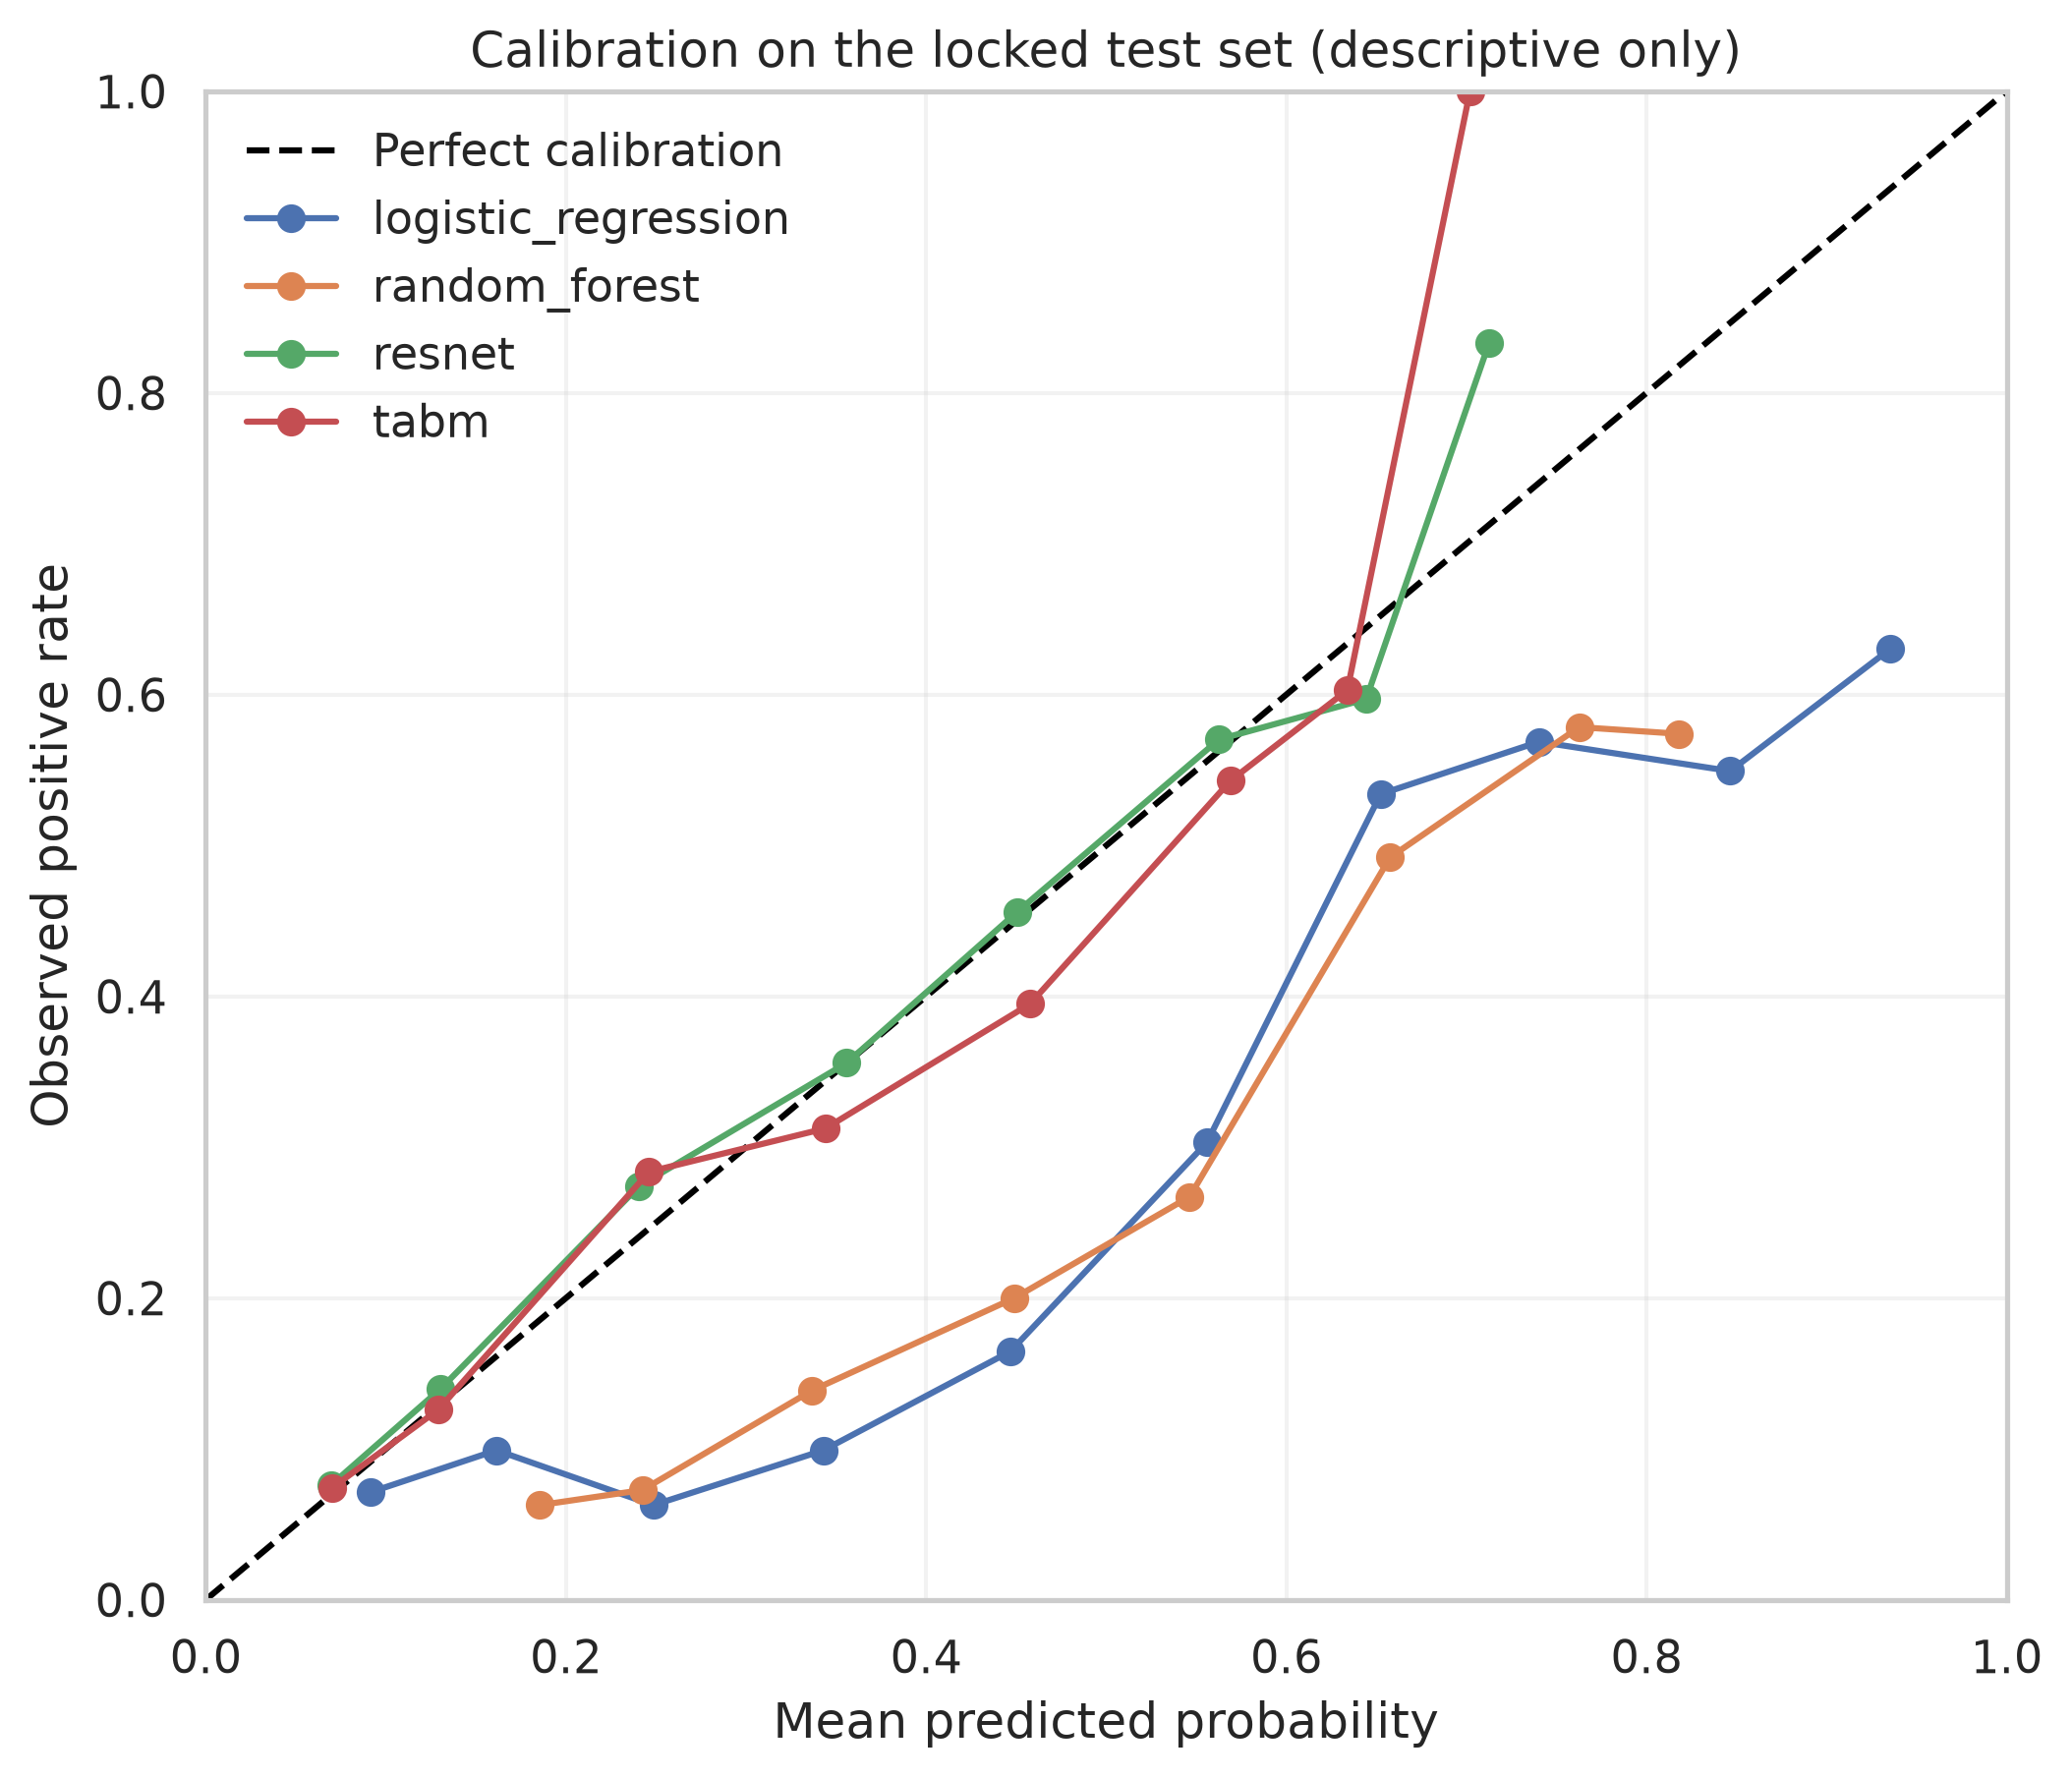
\includegraphics[width=\textwidth]{model_calibration_curves.png}
    \caption{Reliability curves trên test khóa kín.}
  \end{subfigure}
  \caption{Audit độ bất định và calibration; chỉ dùng mô tả sau khi khóa mô hình.}
  \label{fig:robustness-audit}
\end{figure}

ResNet và TabM có Brier score lần lượt 0,1353 và 0,1355, thấp hơn Random Forest 0,1704; ECE 10-bin tương ứng khoảng 0,0155, 0,0146 và 0,1807. Class weighting làm xác suất traditional model lệch khỏi tần suất quan sát, nên không được hiểu trực tiếp như rủi ro tuyệt đối nếu chưa calibration riêng trên dữ liệu ngoài mẫu.

Audit theo giới tính được thực hiện cho Female ($n=214$), Male ($n=1.929$) và Missing ($n=712$). Nhóm Missing có tỷ lệ dương gốc và predicted-positive rate cao hơn; chênh lệch có thể phản ánh cơ chế thiếu dữ liệu. Hình~\ref{fig:gender-audit} mô tả recall, nhưng không đủ để kết luận mô hình công bằng vì nhóm không cân bằng, gender thiếu nhiều và chưa kiểm soát biến nhiễu.

\begin{figure}[H]
  \centering
  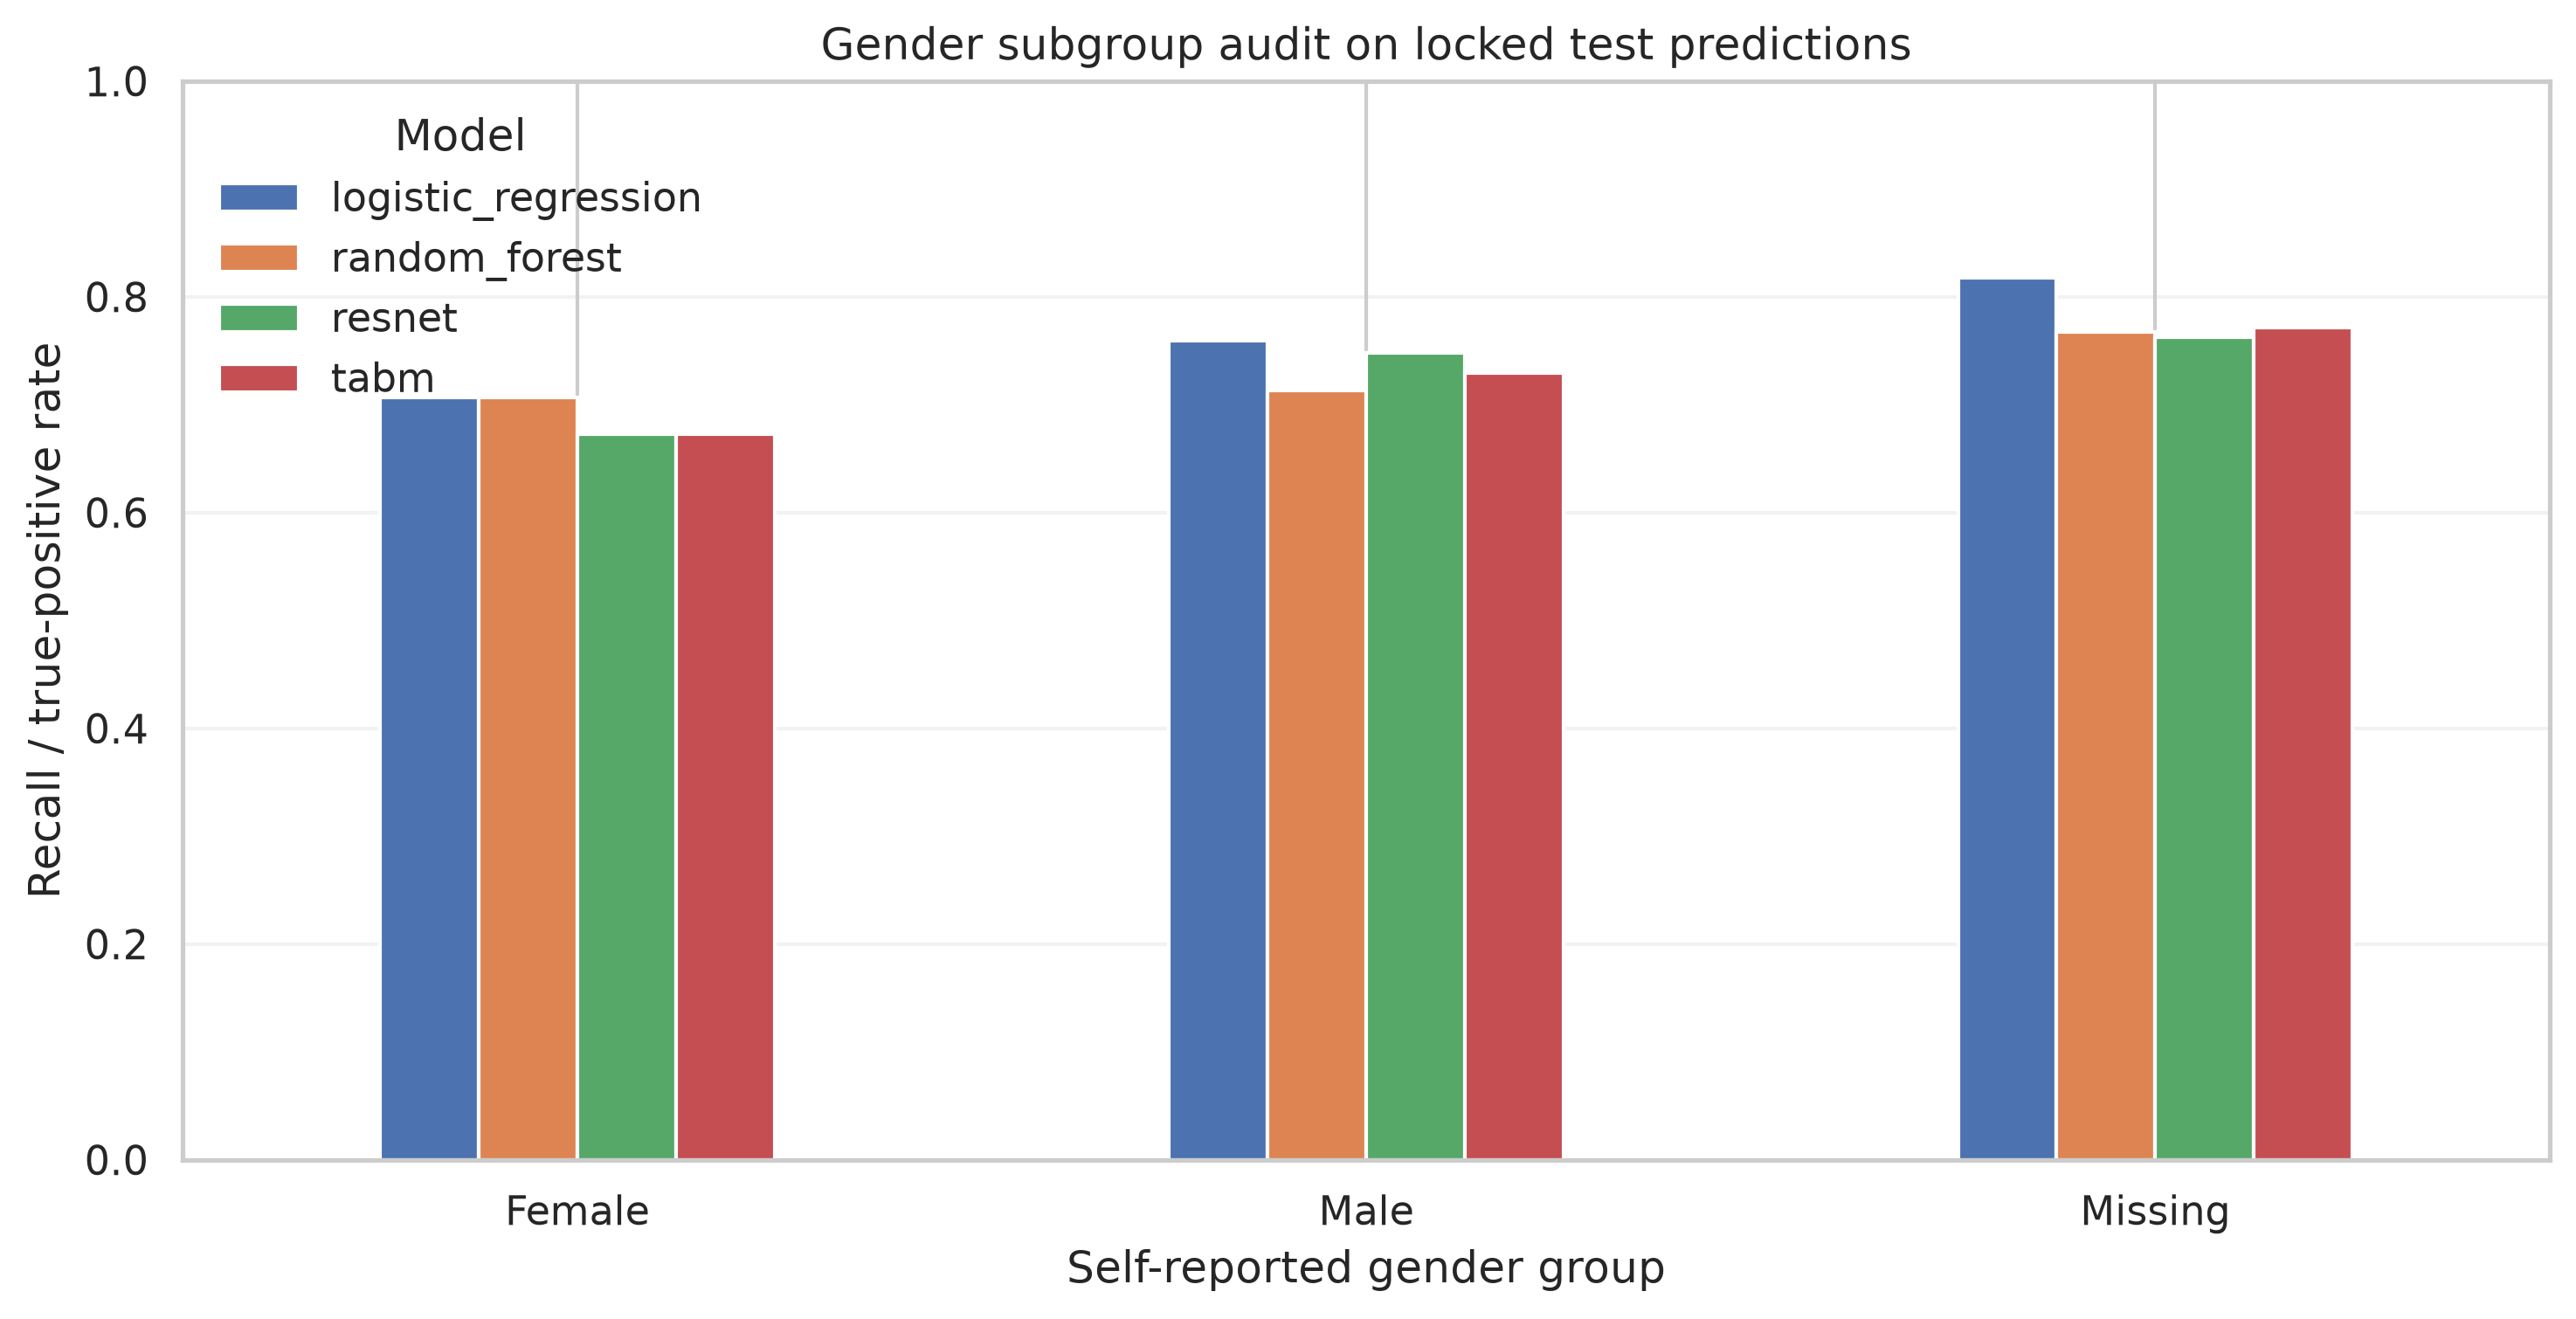
\includegraphics[width=0.86\textwidth]{gender_subgroup_recall.png}
  \caption{Recall theo nhóm giới tính tự khai và nhóm thiếu thông tin.}
  \label{fig:gender-audit}
\end{figure}

\section{Hạn chế và nguy cơ đối với kết luận}

\begin{itemize}
  \item Kết quả test vẫn dựa trên một dataset và một split; repeated CV chỉ kiểm tra cấu hình traditional trên train+validation, chưa thay thế external validation hoặc nested CV đầy đủ.
  \item Nhãn phản ánh ý định chuyển việc trong dữ liệu, không phải kết quả chuyển việc thực tế; có thể tồn tại sai lệch chọn mẫu.
  \item Audit giới tính chỉ là kiểm tra mô tả ban đầu, chưa đánh giá giao cắt nhóm, uncertainty từng nhóm, demographic parity có điều kiện hoặc tác động pháp lý.
  \item Khoảng bootstrap của chênh lệch F1 deep--Random Forest chứa 0; cần dữ liệu mới trước khi khẳng định ưu thế tổng quát.
  \item Feature importance không chứng minh quan hệ nhân quả. Dữ liệu thiếu có thể phản ánh quy trình thu thập thay vì đặc điểm ứng viên.
  \item TabM chứa tám member nội bộ; cả hai deep model phức tạp và khó giải thích hơn baseline.
  \item Phiên bản môi trường ghi nhận trong metadata mới hơn yêu cầu tối thiểu; cần xác nhận lại trên runtime Colab sạch trước khi nộp.
\end{itemize}

\section{Hướng phát triển}

Các hướng tiếp theo gồm external validation theo thời gian/đơn vị; nested cross-validation cho toàn bộ model family; calibration trên tập độc lập; so sánh CatBoost/Gradient Boosting; fairness theo nhóm giao cắt với khoảng tin cậy; và distillation/quantization để giảm chi phí deep model.

% =============================================================================
\chapter{Sản phẩm, tái lập và tổ chức mã nguồn}
% =============================================================================

\section{Google Colab và quy trình chạy}

Frontend chính là \code{notebooks/ML\_Tabular\_Final.ipynb}. Notebook hợp nhất 42 cell và bản lưu hiện tại không chứa output lỗi. Khi chạy trên Colab, notebook clone repository công khai, không mount Google Drive. Các bước EDA, feature extraction, traditional ML, deep learning và lưu artifact được thực hiện theo thứ tự.

\noindent\textbf{Liên kết Colab:} \url{https://colab.research.google.com/github/Puuffiiii/261-ML-Assignment-G3/blob/main/notebooks/ML_Tabular_Final.ipynb}

\noindent\textbf{Liên kết GitHub chính thức:} \url{https://github.com/Puuffiiii/261-ML-Assignment-G3}

\medskip
Notebook tự clone repository công khai, cài \code{requirements.txt}, tải CSV từ URL công khai nếu file vắng và kiểm tra SHA-256 trước khi đọc. Link Kaggle gốc được nêu trực tiếp; không dùng credential hay mount cloud cá nhân. Khi thông tin hành chính đã chốt, các liên kết \code{main} phải được thay bằng tag submission bất biến và kiểm thử \textit{Runtime $\rightarrow$ Run all} trên Colab sạch.

\section{Cấu trúc thư mục}

\begin{lstlisting}
.
|-- configs/       # JSON search spaces
|-- data/          # aug_train.csv va mo ta nguon
|-- features/      # .npy, split indices, preprocessors, metadata
|-- models/        # traditional models, ResNet va TabM checkpoints
|-- modules/       # EDA, preprocessing, modeling, deep learning
|-- notebooks/     # Colab frontend va notebook phu
|-- reports/       # LaTeX/PDF, CSV va figures
|-- scripts/       # audit va cap nhat notebook co the tai lap
|-- tests/         # unit tests
|-- MODEL_CARD.md
|-- requirements.txt
`-- README.md
\end{lstlisting}

Cấu trúc chứa đầy đủ bốn thư mục bắt buộc \code{notebooks/}, \code{modules/}, \code{reports/}, \code{features/}. Các file feature \code{.npy} gồm bốn biểu diễn $\times$ ba split, cùng ba vector nhãn. Model và preprocessor cuối được lưu để tái sử dụng.

\section{Artefact chính}

\begin{longtable}{p{0.37\textwidth} p{0.56\textwidth}}
\caption{Artefact phục vụ kiểm toán và tái lập}\label{tab:artifacts}\\
\toprule
\textbf{Đường dẫn} & \textbf{Nội dung} \\
\midrule
\endfirsthead
\toprule
\textbf{Đường dẫn} & \textbf{Nội dung} \\
\midrule
\endhead
\bottomrule
\endfoot
\code{features/split\_indices.npz} & Chỉ số split 70/15/15, seed 42. \\
\code{features/X\_*\_std.npy} & 39 đặc trưng Standard cho ba split. \\
\code{features/X\_*\_minmax.npy} & 39 đặc trưng MinMax cho ba split. \\
\code{features/X\_*\_pca90.npy} & 22 principal components cho ba split. \\
\code{features/X\_*\_pca95.npy} & 24 principal components cho ba split. \\
\code{features/preprocessors.joblib} & Các transformer đã fit trên train. \\
\code{models/*.joblib} & Logistic Regression và Random Forest cuối. \\
\code{models/resnet.pt}, \code{models/tabm.pt} & State dict và threshold của hai deep model. \\
\code{reports/model\_validation\_results.csv} & Toàn bộ 24 candidate truyền thống. \\
\code{reports/deep\_validation\_results.csv} & Ba candidate ResNet và ba candidate TabM. \\
\code{reports/all\_models\_test\_comparison.csv} & So sánh test cuối của bốn thuật toán. \\
\code{reports/model\_bootstrap\_intervals.csv} & Bootstrap 95\% cho F1, PR-AUC, ROC-AUC. \\
\code{reports/repeated\_cv\_summary.csv} & Độ ổn định cấu hình traditional trên train+validation. \\
\code{reports/gender\_subgroup\_audit.csv} & Audit sai số theo gender/missing. \\
\code{reports/audit\_provenance.json} & Phiên bản, checksum và chính sách audit. \\
\end{longtable}

\section{Kiểm thử}

Bốn module test kiểm tra metric/threshold/persistence của traditional ML, preprocessing/forward/persistence của deep model, contract của calibration/bootstrap/subgroup audit, và tính hợp lệ/tự chứa của notebook. Lần kiểm tra ngày 05/11/2026 ghi nhận 11/11 test thành công trên Python 3.14.7. Trước khi nộp cần chạy lại:

\begin{lstlisting}[language=bash]
python -m unittest discover -s tests -v
\end{lstlisting}

\noindent Kết quả cuối phải được lưu cùng log Run All trên Colab sau khi tag submission được phát hành.

% =============================================================================
\chapter{Phân công công việc và minh chứng nhóm}
% =============================================================================

Theo đề bài, bảng phân công chi tiết và tỷ lệ đóng góp là bắt buộc; điểm cá nhân được tính theo
\[
  \text{Điểm cá nhân}=\text{Điểm nhóm}\times\text{Tỷ lệ đóng góp (\%)}.
\]

Không thể suy ra phân công thực tế chỉ từ lịch sử file. Nhóm cần thống nhất và điền bảng phân công bên dưới; tổng tỷ lệ nên được kiểm tra theo hướng dẫn của GVHD.

\begin{landscape}
\begin{table}[H]
\centering
\caption{Bảng phân công và tỷ lệ đóng góp}\label{tab:contribution}
\begin{tabularx}{\linewidth}{p{0.045\linewidth} p{0.18\linewidth} p{0.095\linewidth} p{0.35\linewidth} p{0.18\linewidth} p{0.065\linewidth}}
\toprule
\textbf{STT} & \textbf{Thành viên} & \textbf{MSSV} & \textbf{Công việc thực tế} & \textbf{Sản phẩm/minh chứng} & \textbf{Tỷ lệ} \\
\midrule
1 & Phạm Hoàng Minh Hiếu & \placeholder{MSSV} & \placeholder{Hạng mục đã thực hiện} & \placeholder{File/commit/biên bản} & \placeholder{\%} \\
2 & Lê Duy Nhật Minh & \placeholder{MSSV} & \placeholder{Hạng mục đã thực hiện} & \placeholder{File/commit/biên bản} & \placeholder{\%} \\
3 & Nguyên Ngô Huy & \placeholder{MSSV} & \placeholder{Hạng mục đã thực hiện} & \placeholder{File/commit/biên bản} & \placeholder{\%} \\
4 & Nguyễn Nhật Thành & 2353102 & \placeholder{Hạng mục đã thực hiện} & \placeholder{File/commit/biên bản} & \placeholder{\%} \\
\bottomrule
\end{tabularx}
\end{table}
\end{landscape}

\section{Thông tin liên hệ}

\begin{table}[H]
\centering
\caption{Thông tin thành viên cần hoàn thiện}\label{tab:member-contact}
\begin{tabularx}{\textwidth}{l l X}
\toprule
\textbf{Họ và tên} & \textbf{MSSV} & \textbf{Email} \\
\midrule
Phạm Hoàng Minh Hiếu & \placeholder{MSSV} & \placeholder{Email trường} \\
Lê Duy Nhật Minh & \placeholder{MSSV} & \placeholder{Email trường} \\
Nguyên Ngô Huy & \placeholder{MSSV} & \placeholder{Email trường} \\
Nguyễn Nhật Thành & 2353102 & \placeholder{Email trường} \\
\bottomrule
\end{tabularx}
\end{table}

\section{Minh chứng làm việc nhóm và báo cáo tiến độ}

\begin{itemize}
  \item Biên bản họp/ảnh/video: \placeholder{Đường dẫn thư mục minh chứng.}
  \item Đăng ký nhóm trên Google Sheet LMS: \placeholder{Ngày/xác nhận đăng ký.}
  \item Báo cáo tiến độ: \placeholder{Danh sách ngày nộp và đường dẫn.}
  \item Xác nhận roster 2--3 thành viên hoặc ngoại lệ bốn thành viên: \placeholder{Phản hồi của GVHD.}
\end{itemize}

% =============================================================================
\chapter{Kết luận}
% =============================================================================

Nhóm đã xây dựng đầy đủ pipeline học máy truyền thống cho dữ liệu bảng theo yêu cầu: EDA, xử lý khuyết và categorical, trích xuất/thiết kế đặc trưng, scaling, PCA, huấn luyện hai thuật toán, tuning nhiều cấu hình và đánh giá test khóa kín. Random Forest là mô hình truyền thống tốt nhất với Accuracy 0,7947, F1 0,6389, ROC-AUC 0,8120 và PR-AUC 0,5414.

Phần mở rộng ResNet đạt PR-AUC 0,5657 và F1 0,6438; TabM đạt PR-AUC 0,5576 và F1 0,6427. Random Forest vẫn có ROC-AUC cao nhất, TabM có Accuracy/Precision cao nhất và Logistic Regression có Recall cao nhất. Bootstrap cho thấy chênh lệch F1 deep--Random Forest còn bất định; vì vậy lựa chọn triển khai phải dựa trên chi phí sai số, calibration, tài nguyên và nhu cầu giải thích.

Pipeline đã lưu feature, split, preprocessor, model, cấu hình, bảng kết quả, audit, checksum và hình. Các việc còn phụ thuộc thông tin bên ngoài là điền metadata/thành viên, đính kèm phân công và minh chứng, xác nhận dataset/roster, chạy Colab sạch, phát hành tag bất biến và nộp theo lịch LMS.

% =============================================================================
\appendix
\chapter{Danh mục kiểm tra trước khi nộp}
% =============================================================================

\begin{itemize}
  \item[$\square$] Không còn chuỗi \textit{CẦN BỔ SUNG} trong PDF.
  \item[$\square$] Danh sách thành viên phù hợp quy định 2--3 người hoặc có xác nhận ngoại lệ.
  \item[$\square$] Bảng phân công có nhiệm vụ, minh chứng và tỷ lệ đóng góp.
  \item[$\square$] Notebook chứa link nguồn dữ liệu, cài thư viện và tải/giải nén tự động.
  \item[$\square$] Colab sạch chạy \textit{Run all} thành công, không mount cloud cá nhân.
  \item[$\square$] Link Colab/GitHub/PDF trỏ đúng branch hoặc tag nộp cuối.
  \item[$\square$] Feature \code{.npy}, module, notebook và report nằm đúng cấu trúc.
  \item[$\square$] Đã chạy test cuối, commit, push và xác minh repository công khai.
  \item[$\square$] Đã nộp báo cáo tiến độ, đăng ký nhóm và package cuối theo LMS.
\end{itemize}

\chapter{Hướng dẫn biên dịch báo cáo}

Từ thư mục \code{reports/}, chạy pdfLaTeX hai lần để cập nhật mục lục và tham chiếu. Source cũng tương thích XeLaTeX/LuaLaTeX trên môi trường có đầy đủ Unicode font packages:

\begin{lstlisting}[language=bash]
pdflatex -interaction=nonstopmode -halt-on-error report_vi.tex
pdflatex -interaction=nonstopmode -halt-on-error report_vi.tex
\end{lstlisting}

File đầu ra là \code{reports/report\_vi.pdf}. Các hình được lấy trực tiếp từ \code{reports/figures/}.

% =============================================================================
\begin{thebibliography}{9}

\bibitem{assignment}
Khoa Khoa học và Kỹ thuật Máy tính, Trường Đại học Bách Khoa, ĐHQG-HCM,
\textit{Bài tập lớn môn học: Học máy, Học kỳ I -- Năm học 2026--2027}, 2026.

\bibitem{kaggledata}
Arash Nic,
\textit{HR Analytics: Job Change of Data Scientists}, Kaggle.
\url{https://www.kaggle.com/datasets/arashnic/hr-analytics-job-change-of-data-scientists}.

\bibitem{pedregosa2011}
F. Pedregosa et al.,
``Scikit-learn: Machine Learning in Python,''
\textit{Journal of Machine Learning Research}, vol. 12, pp. 2825--2830, 2011.

\bibitem{breiman2001}
L. Breiman,
``Random Forests,''
\textit{Machine Learning}, vol. 45, pp. 5--32, 2001.

\bibitem{gorishniy2021}
Y. Gorishniy, I. Rubachev, V. Khrulkov, and A. Babenko,
``Revisiting Deep Learning Models for Tabular Data,''
\textit{Advances in Neural Information Processing Systems}, vol. 34, 2021.

\bibitem{saito2015}
T. Saito and M. Rehmsmeier,
``The Precision--Recall Plot Is More Informative than the ROC Plot When Evaluating Binary Classifiers on Imbalanced Datasets,''
\textit{PLOS ONE}, vol. 10, no. 3, 2015.

\bibitem{gorishniy2025tabm}
Y. Gorishniy, A. Kotelnikov, and A. Babenko,
``TabM: Advancing Tabular Deep Learning with Parameter-Efficient Ensembling,''
\textit{International Conference on Learning Representations}, 2025.
\url{https://openreview.net/forum?id=Sd4wYYOhmY}.

\end{thebibliography}

\end{document}
